\documentclass[12pt]{article} 
\usepackage[american]{babel}
\usepackage{makeidx}
\usepackage{amssymb}
\usepackage{amsmath}
\usepackage{xfrac}
\usepackage{graphicx}
\usepackage{epstopdf}
\usepackage{amsthm}
\usepackage{caption}
\usepackage{subcaption}
\usepackage{enumerate}
\usepackage{cleveref}
\usepackage{framed}

\oddsidemargin= -12pt \evensidemargin= -12pt
\topmargin=-45pt
\binoppenalty=10000
\relpenalty=10000
\textwidth=6.5in\textheight=9in \baselineskip=18pt
\parskip=6pt plus 1pt
\numberwithin{equation}{section}

\newtheorem{proposition}{Proposition}[section]
\newtheorem{lemma}{Lemma}[proposition]
\newtheorem{remark}{Remark}
\newtheorem{assumption}{Assumption}
\newtheorem{definition}{Definition}
\newtheorem{theorem}{Theorem}

\newcommand{\nn}{\mathbb{N}} %Nonnegative integers
\newcommand{\rr}{\mathbb{R}} %Real numbers
\newcommand{\norm}[1]{\left\Vert {#1} \right\Vert} %Norm
\def\abs#1{\left\lvert#1\right\rvert}
\makeatletter
\def\Let@{\def\\{\notag\math@cr}}
\makeatother

\begin{document}

%\begin{center} 
%\Large {Tel-Aviv University}
%
%\Large {The Raymond and Beverly Sackler Faculty of} \\
%\Large {Exact Sciences} \\
%\Large {The Department of Statistics and Operations} \\
%\Large {Research}
%
%\bigskip
%\bigskip
%\bigskip
%
%\Large {\bf Draft }
%
%\bigskip
%\bigskip
%\bigskip
%\bigskip
%
%\Large{Thesis Submitted Towards the Degree of Master} \\
%\Large {of Science in Operations Research}
%
%\bigskip
%
%\Large {Sergey Voldman}
%
%\bigskip
%\bigskip
%\bigskip
%
%\Large {Supervisors:} \\
%\Large {Prof. Marc Teboulle} \\
%\Large {Prof. Shoham Sabach}
%
%\bigskip
%\bigskip
%
%\Large{2016}
%
%\end{center}
%
%\newpage
%
%\begin{center} \Large {\bf Draft}
%\end{center}
%
%\begin{abstract} 
%
%To-do...
%
%\newpage
%
%\end{abstract}
%
%\section{Introduction}
%
%To-do...
%

\tableofcontents
\clearpage
{%
\let\oldnumberline\numberline%
\renewcommand{\numberline}{\figurename~\oldnumberline}%
\listoffigures%
}
\clearpage
%\listoftables
%\clearpage

\section{Introduction}

The clustering problem is the task of grouping objects which are similar. It consists of partitioning a dataset into subsets, called clusters, such that the data points in each cluster are similar with respect to a specific criteria. 

The clustering problem is a fundamental problem in machine learning field, and it arises in wide scope of applications, such as data mining, pattern recognition, information retrieval and many others. For example, in image segmentation, one is interested in partitioning the pixels of an image into objects, where each pixel can be described via its location in the image and its color given in RGB format. Another example is learning the probability density of some data, where the data is assumed to be drawn from a mixtures of distributions. Each partition of the data is represented by a unimodal probability density model, and summing of all the cluster models gives a multimodal density for the entire dataset. Vector quantization is yet another example, where large sets of points are represented by their centroid point. This method can be used for data compression, data correction and pattern recognition.

There are several categories of clustering methods, each has a direct impact of the final clustering structure.
\begin{enumerate}[(i)]
	\item Hierarchical versus partitioning clustering: In partitioning clustering the dataset is divided into clusters, whereas in hierarchical clustering each cluster may have sub-clusters, thus forming a tree which leaves are the single points of the dataset.
	\item Hard versus soft and fuzzy clustering: In hard clustering each data point is assigned to single cluster, versus a soft clustering where each point may be assigned to more than one cluster, hence clusters may overlap. In fuzzy clustering for each point there is a distribution that describes the probability of a point to be part of a cluster.
	\item Complete versus partial clustering: In complete clustering all points in the dataset are assigned to clusters, whereas in partial clustering some points may be intentionally skipped and are not being assigned to a cluster.
\end{enumerate}

Finding the optimal partition of a fixed number of clusters for some given dataset is known to be a NP-hard problem, and hence cannot be solved efficiently. Most algorithms seek to minimize some mathematical criteria, and usually achieve local rather than global minimum solution. In this work we focus on partitioning clustering, where the number of clusters in known in advance. Most partitioning clustering methods iteratively update the cluster centers, and hence they are often referred as center-based clustering methods. We introduce few notations for the upcoming discussion. Let $\mathcal{A}= \left\lbrace a^1, a^2, \ldots ,a^m \right\rbrace$ be a given set of points in $\mathbb{R}^n$, and let $1 < k < m$ be a fixed given number of clusters. The clustering problem consists of partitioning the dataset $\mathcal{A}$ into $k$ subsets $\left\lbrace C^1, C^2, \ldots ,C^k \right\rbrace$, called clusters. For each $l=1, 2, \ldots ,k$, the cluster $C^l$ is represented by its center $x^l \in \mathbb{R}^n$. We describe several well-known center-based clustering algorithms.
\begin{enumerate}[(i)]
	\item K-means algorithm: This algorithm is probably the most famous within the clustering scope, and dates back to MacQueen (1967). The k-means algorithm partitions the data into $k$ sets. The solution is then a set of $k$ centers, each of which is located at the centroid of the data for which it is the closest center. The k-means algorithm performs hard clustering, and each point is labeled according to its closest center. The objective function that the k-means algorithm minimizes is
	\begin{equation*}
		f_{KM}(x) = \sum\limits_{i=1}^{m}\min\limits_{1 \le l \le k} \norm{a^i-x^l}^2.
	\end{equation*}
	The simplicity of the algorithm both in the theoretical and implementation aspects made it very popular.
	\item Fuzzy k-means (FKM) algorithm: The FKM algorithm is a soft clustering method. For each data point the result of the FKM algorithm is a distribution of membership over the clusters. The objective function that the FKM algorithm minimizes is
	\begin{equation*}
		f_{FKM}(x) = \sum\limits_{i=1}^{m}\sum\limits_{l=1}^{k}(w^i_l)^\beta \norm{a^i-x^l}^2.
	\end{equation*}
	The parameter $w^i_l$ denotes the probability that data point $a^i$ is assigned to cluster $x^l$, thus it is under the constraints $\sum_{l=1}^{k} w^i_l = 1$ for all $1 \leq i \leq m$ and $w^i_l \geq 0$. The parameter $\beta > 1$ governs the "fuzzy partition". Setting $\beta = 1$ results in the standard k-means algorithm.
	\item Expectation-Maximization (EM) algorithm: The EM algorithms is used extensively in statistical estimation problems for learning mixtures of distributions. It is a soft clustering algorithm. The objective function that EM maximizes is 
	\begin{equation*}
		f_{EM} = \sum\limits_{i=1}^{m} \log \left( \sum\limits_{l=1}^{k} p\left(a^i|x^l\right) p\left(x^l\right) \right),
	\end{equation*}
	where  $p\left(a^i|x^l\right)$ is the probability of $a^i$ given that it is generated by the Gaussian distribution with center $x^l$ and $p\left(x^l\right)$ is the prior probability of center $x^l$.
\end{enumerate}
An interesting paper of Teboulle \cite{T2007} shows that these center-based clustering algorithms can be recovered from the proposed continuous optimization framework. The smoothing methodologies for the clustering problem are based on nonlinear means and on approximation of appropriate asymptotic functions.

Most of the existing clustering methods are sensitive to the starting point, namely choosing different starting point result in significant changes in the final clustering. There are plethora of heuristic initialization method. One such initialization method is choosing random $k$ data points as a staring centers for clustering, assuming uniform distribution or some other prior distribution on the data. Another popular method is k-means++, where the first center is chosen at random from the dataset, and for each $2 \leq l \leq k$, the center $x^l$ is the furthest point from the points chosen so far.

%In this work we focus on partitioning clustering, where the number of clusters in known in advance. Most partitioning clustering methods iteratively update the cluster centers, and hence they are often referred as center-based clustering methods. These clustering methods are usually classified as \textit{hard} and \textit{soft}, depending on the way the data points are assigned to clusters. Hard clustering produces a disjoint partition of the data, namely each point is assigned to exactly one cluster. Soft clustering is a relaxation of the disjoint partition demand, and it allows overlapping of the clusters.
%
%The first important category of clustering algorithms is the iterative optimization clustering algorithms. It includes algorithms such as the \textit{k-means} and the \textit{Expectation-Maximization} (EM) algorithms and many more. The k-means algorithm is a very popular data clustering algorithm. It iteratively locates the 

% There exist many approximation algorithms and even more heuristic approaches for the clustering problem. In this work we study the hard clustering center-based method from continuous optimization perspective. 
The starting point of our work is a formulation of the clustering problem which consists of minimizing the sum of finite collection of min-functions, which is a nonsmooth and nonconvex optimization problem, in its most the general case. The clustering problem is given by
\begin{equation}
	\min\limits_{x \in \mathbb{R}^{nk}} \left\lbrace F(x) := \sum\limits_{i=1}^{m} \min\limits_{1 \le l \le k} d(x^l,a^i) \right\rbrace , \label{StateEq1}
\end{equation}
\noindent with $\textit{d}(\cdot ,\cdot)$ being a distance-like function.

%Let $\mathcal{A}= \left\lbrace a^1, a^2, \ldots ,a^m \right\rbrace$ be a given set of points in $\mathbb{R}^n$, and let $1 < k < m$ be a fixed given number of clusters. The clustering problem consists of partitioning the dataset $\mathcal{A}$ into $k$ subsets $\left\lbrace C^1, C^2, \ldots ,C^k \right\rbrace$, called clusters. For each $l=1, 2, \ldots ,k$, the cluster $C^l$ is represented by its center $x^l \in \mathbb{R}^n$, and we are interested to determine $k$ cluster centers $\left\lbrace x^1, x^2, \ldots ,x^k \right\rbrace$ such that the sum of certain proximity measures from each data point $a^i$, $i=1, 2, \ldots ,m$, to a nearest cluster center $x^l$ is minimized. We define the vector of all centers by  $x = (x^1, x^2, \ldots , x^k) \in \mathbb{R}^{nk}$.

The lack of smoothness in this formulation can be overcome, yet the nonconvex nature of the clustering problem shall accompany the discussions throughout this work. Significant amount of studies have been made on convex models, even though in many cases the original optimization problem is nonconvex. To overcome the lack of convexity the common approach is usually achieved by relaxation of the original problem. Motivated by papers of Attouch et al. \cite{AB2009, ABS2013} that established convergence of the sequences generated by the proximal Gauss-Seidel scheme in the general nonconvex and nonsmooth settings, and similar result for the proximal-forward-backward algorithm applied to the nonconvex and nonsmooth minimization of the sum of a nonsmooth function with a smooth one. This approach assumes that the objective function to be minimized satisfies the Kurdyka-{\L}ojasiewicz (KL) property. The convergence results were further extended in the recent work by Bolte et al. \cite{BST2014}, where the objective function is a function of finite blocks of variables. 

We focus on two cases of distance-like functions. The first is the squared Euclidean norm, which is the standard proximity measure used by k-means. For this case, we derive an equivalent smooth optimization problem for the clustering problem presented in (\ref{StateEq1}) and prove our convergence result for the suggested algorithm via the methodology which is discussed in \cite{BST2014}. The second distance-like function that we study is the Euclidean norm. In this case we present two approximations, in order to overcome the lack of smoothness in the problem, and then proceed with the same methodology as in the first case. We present numeric experiments, that show the superiority of the Euclidean norm distance function for datasets in which the data points are spread relatively sparsely form their centers.

\noindent \textbf{Outline of the thesis.} This work is organized as follows. In the following section we transform the initial formulation  of the clustering problem into a smooth one. In addition, we introduce 
the KL theory and the general methodology that will be used in our analysis of the proposed algorithms. In section 3 and 4 we suggest two algorithms, KPLAM and $\varepsilon$-KPALM, respectively. KPALM addresses the clustering problem with squared Euclidean norm distance-like function and $\varepsilon$-KPALM the standard Euclidean norm distance function. Employing the methodology of Section 2 we establish our convergence results.  In section 5 we prove the convergence of k-means algorithm to a critical point and under certain assumption extend the convergence to a local minimum. Finally, in Section 6 we compare the performance of these algorithm according to some common criteria.

\section{Problem Reformulation and Mathematical Tools}

\subsection{Reformulation of the Clustering Problem}

We begin with a reformulation of the clustering problem which will be the basis for our developments in this work. The reformulation is based on the following fact:
\begin{equation*}
	\min\limits_{1 \leq l \leq k} u_l = \min \left\lbrace \langle u,v \rangle : v \in \Delta \right\rbrace ,
\end{equation*}
where $\Delta$ denotes the well-known simplex defined by
\begin{equation*}
	\Delta = \left\lbrace u \in \mathbb{R}^k : \sum\limits_{l=1}^{k} u_l = 1, \: u \geq 0 \right\rbrace .
\end{equation*}
Using this fact in Problem (\ref{StateEq1}) and introducing new variables $w^i \in \mathbb{R}^k$, $i=1,2, \ldots, m$, gives a smooth reformulation of the clustering problem
\begin{equation}
	\min\limits_{x \in \mathbb{R}^{nk}} \sum\limits_{i=1}^{m} \min\limits_{w^i \in \Delta} \langle w^i , d^i(x) \rangle , \label{StateEq2}
\end{equation}
where 
\begin{equation*}
d^{i}(x) = (d(x^1,a^i), d(x^2,a^i), \ldots , d(x^k,a^i)) \in \mathbb{R}^k, \quad i=1, 2, \ldots , m.
\end{equation*}
Replacing further the constraint $w^i \in \Delta$ by adding the indicator function $\delta_{\Delta}(\cdot)$, which is defined to be $0$ in $\Delta$ and $\infty$ otherwise, to the objective function, results in a equivalent formulation
\begin{equation}
	\min\limits_{x \in \mathbb{R}^{nk} , w \in \mathbb{R}^{km}} \left\lbrace \sum\limits_{i=1}^{m} \left( \langle w^i , d^i(x) \rangle + \delta_{\Delta}(w^i) \right) \right\rbrace , \label{StateEq3}
\end{equation}
where $w = (w^1, w^2, \ldots , w^m) \in \mathbb{R}^{km}$.
Finally, for the simplicity of the yet to come expositions, we define the following functions
\begin{center}
$H(w,x) := \sum\limits_{i=1}^{m} H^i(w,x) = \sum\limits_{i=1}^{m} \langle w^i , d^i(x) \rangle \quad$ and $\quad G(w) = \sum\limits_{i=1}^{m} G^i(w^i) := \sum\limits_{i=1}^{m} \delta_{\Delta}(w^i) .$
\end{center}

Replacing the terms in Problem (\ref{StateEq3}) with the functions defined above gives a compact equivalent form of the original clustering problem

\begin{equation}
	\min \left\lbrace \Psi(z) := H(w,x) + G(w) \mid z := (w,x) \in \mathbb{R}^{km} \times \mathbb{R}^{nk} \right\rbrace . \label{StateEq4}
\end{equation}

\subsection{Introduction to the PALM Theory} \label{State_PALM_Theory}

In this subsection we give a brief review of the main developments established in \cite
{BST2014}. These developments which include the proximal alternating linearized minimization (PALM) algorithm and general procedure for proving global convergence of generic algorithm play a central rule in this work. First, let us recall several definitions which are needed for the upcoming discussion.

\begin{definition}[Subdifferentials]
	Let $\sigma : \rr^d \rightarrow (-\infty,+\infty]$ be a proper and lower semicontinuous function.
	\begin{enumerate}[(i)]
		\item For a given $x \in dom\;\sigma := \left\lbrace x \in \rr^d : \; \sigma(x) < \infty \right\rbrace$, the \textit{Fr\'echet subdifferential} of $\sigma$ at $x$, written $\widehat{\partial}\sigma(x)$, is the set of all vectors $u \in \rr^d$ which satisfy
		\begin{equation*}
			\lim\limits_{y \neq x} \inf\limits_{y \rightarrow x} \frac{\sigma(y) - \sigma(x) - \left\langle u, y-x \right\rangle}{\norm{y-x}} \geq 0.
		\end{equation*}
		When $x \notin dom\sigma$, we set $\widehat{\partial}\sigma(x) = \emptyset$.
		\item The \textit{limiting-subdifferential}, or subdifferential in short, of $\sigma$ at $x \in \rr^n$, written $\partial\sigma(x)$, is defined through the following closure process
		\begin{equation*}
			\partial\sigma(x) := \left\lbrace u \in \rr^d : \exists x^k \rightarrow x, \; \sigma(x^k)\rightarrow \sigma(x) \text{ and } u^k \in \widehat{\partial}\sigma(x^k) \text{ as } k \rightarrow \infty \right\rbrace.
		\end{equation*}
	\end{enumerate}
\end{definition}
In the nonsmooth context, as in the smooth case, the well-known Fermat's rule remains unchanged, that is, if $x \in \rr^d$ is a local minimizer of $\sigma$ then $0 \in \partial\sigma(x)$. Points whose subdifferential contains $0$ are called \textit{critical points}, and the set of all critical points of $\sigma$ is denoted by crit$\sigma$.

Now we present the Kurdyka-{\L}ojasiewicz property, which plays a central role in PALM's analysis. Let $\eta \in (0,+\infty]$. Denote the following class of functions
\begin{equation*}
	\Phi_{\eta} = \left\lbrace \varphi \in C\left([0,\eta), \rr_+ \right)  , concave : \; \varphi \in C^1\left((0,\eta)\right), \; \varphi'>0, \; \varphi(0)=0 \right\rbrace .
\end{equation*}
%Denote by $\Phi_{\eta}$ the class of all concave and continuous functions $\varphi:[0,\eta) \rightarrow \rr_+$ which satisfy the following conditions
%\begin{enumerate}[(i)]
%	\item $\varphi(0)=0$;
%	\item $\varphi$ is $C^1$ on $(0,\eta)$ and continuous at $0$;
%	\item for all $s \in (0,\eta): \; \varphi'(s)>0$.
%\end{enumerate}
\begin{definition}[Kurdyka-{\L}ojasiewicz property]
	Let $\sigma: \rr^d \rightarrow (-\infty,+\infty]$ be proper and lower semicontinuous.
	\begin{enumerate}[(i)]
		\item The function $\sigma$ is said to have the \textit{Kurdyka-{\L}ojasiewicz (KL) property} at $\overline{u} \in dom \; \partial\sigma := \\ \left\lbrace u \in \rr^d : \; \partial\sigma \neq \emptyset \right\rbrace$ if there exist $\eta \in (0,+\infty]$, a neighborhood $U$ of $\overline{u}$ and a function $\varphi \in \Phi_{\eta}$, such that for all
		\begin{equation*}
			u \in U \cap \left\lbrace x \in \rr^d : \; \sigma(\overline{u}) < \sigma(x) < \sigma(\overline{u}) + \eta \right\rbrace,
		\end{equation*}
		the following inequality holds
		\begin{equation*}
			\varphi'(\sigma(u) - \sigma(\overline{u}))dist(0,\partial\sigma(u)) \geq 1,
		\end{equation*}
		where $dist(x,S) := \inf \left\lbrace \norm{y-x} : \; y \in S\right\rbrace$ denotes the distance from $x \in \rr^d$ to $S \subset \rr^d$.
		\item If $\sigma$ satisfy the KL property at each point of $dom\;\sigma$ then $\sigma$ is called a \textit{KL function}.
	\end{enumerate}
\end{definition}

\begin{definition}[Semi-algebraic sets and functions] 
\begin{enumerate}[(i)]
	\item A subset $S \subset \rr^d$ is a real semi-algebraic set if there exists a finite number of real polynomial functions $g_{ij}, h_{ij}: \rr^d \rightarrow \rr$ such that
	\begin{equation*}
		S = \bigcup\limits_{j=1}^{p} \bigcap\limits_{i=1}^{q} \left\lbrace u \in \rr^d : \; g_{ij}=0 \text{ and } h_{ij}(u)<0 \right\rbrace
	\end{equation*}
	\item A function $h:\rr^d \rightarrow (-\infty, +\infty]$ is called semi-algebraic if its graph
	\begin{equation*}
		\left\lbrace (u,t)\in\rr^{d+1} : \; h(u)=t \right\rbrace
	\end{equation*}
	is a semi-algebraic subset of $\rr^{d+1}$.
\end{enumerate}
\end{definition}

\begin{theorem} \label{SA_is_KL}
Let $\sigma:\rr^d \rightarrow (-\infty, +\infty]$ be a proper and lower semicontinuous function. If $\sigma$ is semi-algebraic then if satisfies the KL property at any point of dom $\sigma$.
\end{theorem}
The class of semi-algebraic function is very broad, it includes real polynomial functions; indicator functions of semi-algebraic sets; finite sums and products of semi-algebraic functions; composition of semi-algebraic functions, and many more.

Equipped with these definitions, we present the methodology that was used for PALM algorithm, and will be used several times throughout this work. Let $\Psi : \rr^d \rightarrow ( -\infty, +\infty ]$ be a proper and lower semicontinuous function which is bounded from below and consider the problem
\begin{equation*}
	(P) \quad \left\lbrace \Psi(z) : z \in \rr^d \right\rbrace .
\end{equation*} 
Suppose that we are given a generic algorithm $\mathcal{A}$ which generates a sequence $\left\lbrace z^k \right\rbrace_{k \in \mathbb{N}}$ via the following scheme:
\begin{equation*}
	z^0 \in \mathbb{R}^d, \: z^{k+1} \in \mathcal{A}\left(z^k\right), \quad k=0,1,\ldots.
\end{equation*}
Building upon \cite{AB2009,ABS2013}, the following three requirements are sufficient to assure the convergence of the whole sequence $\left\lbrace z^k \right\rbrace_{k \in \mathbb{N}}$ to a critical point of $\Psi$.
\begin{enumerate}[(C1)]
	\item \textit{Sufficient decrease property:} There exists a positive constant $\rho_1$, such that
	\begin{equation*}
		\rho_1 \|z^{k+1} - z^k\|^2 \leq \Psi(z^k) - \Psi(z^{k+1}), \quad \forall \: k=0,1,\ldots .
	\end{equation*} \label{C1}
	\item \textit{A subgradient lower bound for iterates gap:} Assuming that the sequence generated by the algorithm $\mathcal{A}$ is bounded. There exists a positive constant $\rho_2$, such that
	\begin{equation*}
		\|w^{k+1}\| \leq \rho_2 \|z^{k+1} - z^k\|, \quad w^k \in \partial \Psi\left( z^k \right) \quad \forall \: k=0,1,\ldots .
	\end{equation*} \label{C2}
%	where $\partial \Psi(x)$ is the limiting-subdifferential, defined through the following closure process
%	\begin{equation*}
%		\partial \Psi(x) := \left\lbrace \exists \; x^k \rightarrow x, \; \Psi\left(x^k\right) \rightarrow \Psi\left(x\right) \text{ and } u^k \in \widehat{\partial}\Psi(x^k) \rightarrow u \text{ as } k \rightarrow \infty \right\rbrace,
%	\end{equation*}
%	and $\widehat{\partial}\Psi(x)$ is the set of all vectors $u \in \rr^d$ which satisfy
%	\begin{equation*}
%		\lim\limits_{y \neq x} \inf\limits_{y \rightarrow x} \frac{\Psi(y) - \Psi(x) - \left\langle u, y-x \right\rangle}{\norm{y-x}} \geq 0.
%	\end{equation*}
	\item \textit{KL property:} The function $\Psi$ is a KL function. \label{C3} 
\end{enumerate}
%With regard to the last item, see the definition of KL property in [BST2014]. The objective functions to be discussed in the current work are all KL functions, since it is either a weighed sum of squared Euclidean norms, or a weighed sum of Euclidean norms.

Due to \Cref{SA_is_KL}, property (C3) follows whenever $\Psi$ is a semi-algebraic function. Finally, we present the proximal alternating linearized minimization (PALM) algorithm which solves the nonconvex and nonsmooth minimization problem of the following form
\begin{center}
(\textit{M})\quad minimize $\Psi(x,y):=f(x)+g(y)+H(x,y)$ over all $(x,y) \in \mathbb{R}^n \times \mathbb{R}^m$,
\end{center}
where $f:\mathbb{R}^n \rightarrow \left(-\infty,+\infty\right]$ and $g:\mathbb{R}^n \rightarrow \left(-\infty,+\infty\right]$ are proper and lower semicontinuous functions while $H:\mathbb{R}^n \times \mathbb{R}^m \rightarrow \mathbb{R}$ is a $C^1$ function. In addition, partial gradients of $H$ are Lipschitz continuous, namely, $H(\cdot, y) \in C^{1,1}_{L_1(y)}$ and $H(x,\cdot) \in C^{1,1}_{L_2(x)}$.
PALM is alternating the steps of the proximal forward-backward (PFB) scheme. PFB scheme tackles the problem of minimizing the sum of a smooth function $h$ with a nonsmooth one $\sigma$, and can be viewed as the proximal regularization of $h$ linearized at a given point $x^k$, that is,
\begin{equation*}
	x^{k+1} \in \arg\!\min_{x \in \rr^d} \left\lbrace \left\langle x - x^k, \nabla h\left(x^k\right) \right\rangle + \frac{t}{2}\norm{x-x^k}^2 + \sigma(x)\right\rbrace,\; (t>0).
\end{equation*}
Adopting this scheme on the two blocks $(x,y)$ leads towards the following approximations 
\begin{equation*}
	\widehat{\Psi}\left(x,y^k\right) = \left\langle x-x^k, \nabla_x H\left( x^k, y^k \right)\right\rangle + \frac{c^k}{2}\norm{x-x^k}^2 + f(x), \; (c_k>0),
\end{equation*}
and
\begin{equation*}
	\widetilde{\Psi}\left(x^{k+1},y\right) = \left\langle y-y^k, \nabla_y H\left( x^{k+1}, y^k \right)\right\rangle + \frac{d^k}{2}\norm{y-y^k}^2 + g(y), \; (d_k>0).
\end{equation*}
Thus, PALM is alternating between the following two subproblems
\begin{center}
$x^{k+1} \in \arg\!\min \left\lbrace \widehat{\Psi}(x,y^k) : \; x \in \rr^n \right\rbrace$ \quad and \quad $y^{k+1} \in \arg\!\min \left\lbrace \widetilde{\Psi}\left(x^{k+1},y\right) : \; y \in \rr^m \right\rbrace$.
\end{center}
Assuming $\Psi$ is KL function and the generated sequence by PALM, $\left\lbrace z^k:=\left( x^k, y^k\right)\right\rbrace_{k \in \nn}$, is bounded, Bolte et al. \cite{BST2014} proved that the sequence obeys properties (C1) and (C2), and it converges to a critical point of $\Psi$. 
%Bolte et al. \ref{BST2014} proved the properties (C1) and (C2), assuming $\Psi$ is KL function and the generated sequence by PALM, $\left\lbrace z^k:=\left( x^k, y^k\right)\right\rbrace_{k \in \nn}$, is bounded, and they further established the convergence of $\left\lbrace z^k\right\rbrace_{k \in \nn}$ to a critical point of $\Psi$.

\section{Clustering: The Squared Euclidean Norm Case} \label{State_Clustering_SqNorm}
\subsection{Clustering with PALM}

In this section we tackle the clustering problem, given in (\ref{StateEq4}), for which the proximity function $d(\cdot,\cdot)$ is taken to be the classical distance function defined by $d(u,v) = \|u-v\|^2$. We devise a PALM-like algorithm, based on the discussion in the previous subsection.
Since the clustering problem has a specific structure, we are ought to exploit it in the following manner.
\begin{enumerate}[(1)]
	\item The function $w \mapsto H(w,x)$, for fixed $x$, is linear and therefore there is no need to linearize it as suggested in the framework which was discussed in \Cref{State_PALM_Theory}.
	\item The function $x \mapsto H(w,x)$, for fixed $w$, is quadratic and convex. Hence, there is no need to add a proximal term as suggested in the framework which was discussed in \Cref{State_PALM_Theory}.
\end{enumerate}

As in the PALM algorithm, our algorithm is based on the old approach of alternating minimization, with the following adaptations which are motivated by the observations mentioned above. More precisely, with respect to $w$ we suggest to regularize the first subproblem with proximal term as follows
\begin{equation}
	w^i(t+1) = \arg\!\min\limits_{w^i \in \Delta} \left\lbrace \langle w^i , d^i(x(t)) \rangle + \frac{\alpha_i(t)}{2} \|w^i - w^i(t)\|^2 \right\rbrace, \quad i=1,2, \ldots, m , \label{State_w_update}
\end{equation}
where $\alpha_i(t) > 0$ for all $i=1,2, \ldots, m$. On the other hand, with respect to $x$ we perform exact minimization, that is,
\begin{equation}
	x(t+1) = \arg\!\min \left\lbrace H(w(t+1), x) \mid x \in \mathbb{R}^{nk} \right\rbrace . \label{State_x_update}
\end{equation}
It is easy to check that all subproblems, with respect to $w^i$, $i=1,2, \ldots, m$, and $x$, can be rewritten explicitly (where we use $P_{\Delta}$ for the orthogonal projection onto the set $\Delta$). Thus, we can present now the KPALM algorithm.
%as follows:
%\begin{equation}
%w^i(t+1) = P_{\Delta} \left(w^i(t) - \frac{d^i(x(t))}{\alpha_i(t)}\right) , \quad i=1, 2, \ldots ,m , \label{StateEq7}
%\end{equation}
%where $P_{\Delta}$ is the orthogonal projection onto the set $\Delta$, and
%\begin{equation}
%x^l(t+1) = \frac{\sum_{i=1}^{m} w^i_l(t+1) a^i}{\sum_{i=1}^{m} w^i_l(t+1)} , \quad l=1, 2, \ldots ,k . \label{StateEq8}
%\end{equation}
%Therefore we can record now the suggested KPALM algorithm.
\begin{framed}
\noindent \textbf{KPALM}
\begin{enumerate}[(1)]
	\item Initialization: $(w(0),x(0)) \in \Delta^m \times \mathbb{R}^{nk} .$
	\item General step $\left( t=0,1, \ldots \right)$:
	\begin{enumerate}[(2.1)]
		\item Cluster assignment: choose certain $\alpha_i(t) > 0$, $i=1,2, \ldots, m$, and compute
		\begin{equation}
			w^i(t+1) = P_{\Delta} \left(w^i(t) - \frac{d^i(x(t))}{\alpha_i(t)}\right) . \label{StateEq5}
		\end{equation}
		\item Center update: for each $l=1, 2, \ldots ,k$ compute
		\begin{equation}
			x^l(t+1) = \frac{\sum_{i=1}^{m} w^i_l(t+1) a^i}{\sum_{i=1}^{m} w^i_l(t+1)} . \label{StateEq6}
		\end{equation}
	\end{enumerate}
\end{enumerate}
\end{framed}

We begin our analysis of the KPALM algorithm with the following boundedness property of the generated sequence. For simplicity, from now on, we denote $z(t):=\left( w(t),x(t) \right)$, $t \in \mathbb{N}$.
\begin{proposition}[Boundedness of KPALM sequence] \label{boundedness_prop}
Let $\left\lbrace z(t) \right\rbrace_{t \in \mathbb{N}}$ be the sequence generated by KPALM. Then, the following statements hold true.
\begin{enumerate}[(i)]
	\item For all $l=1, 2, \ldots ,k$, the sequence $\left\lbrace x^l(t) \right\rbrace_{t \in \mathbb{N}}$ is contained in $Conv(\mathcal{A})$, the convex hull of $\mathcal{A}$, and therefore bounded by $M = \max\limits_{1 \leq i \leq m} \| a^i \|$. \label{boundedness_prop_1}
	\item The sequence $\left\lbrace z(t) \right\rbrace_{t \in \mathbb{N}}$ is bounded in $\mathbb{R}^{km} \times \mathbb{R}^{nk}$.
\end{enumerate}
\end{proposition}

\begin{proof}
\begin{enumerate}[(i)]
	\item  Let $1\leq l \leq k$. We set $\lambda_i = w^i_l(t)/\sum\limits_{j=1}^{m} w^j_l(t), i=1, 2, \ldots ,m$, then $\lambda_i \geq 0$ and $\sum\limits_{i=1}^{m} \lambda_i = 1$. From (\ref{StateEq6}) we have
	\begin{equation}
		x^l(t) = \frac{\sum_{i=1}^{m} w^i_l(t) a^i}{\sum_{i=1}^{m} w^i_l(t)} 
		= \sum_{i=1}^{m} \left( \frac{ w^i_l(t)}{\sum_{j=1}^{m} w^j_l(t)} \right) a^i 
		= \sum\limits_{i=1}^{m} \lambda_i a^i \in Conv(\mathcal{A}), \label{StateBound}
	\end{equation}
	which proves that $x^l(t)$ is in the convex hull of $\mathcal{A}$, for all $l = 1, 2, \ldots, k$ and $t \in \mathbb{N}$. Taking the norm of $x^l(t)$ and using (\ref{StateBound}) yields that
	\begin{equation*}
		\| x^l(t) \| = \left\lVert \sum_{i=1}^{m} \lambda_i a^i \right\lVert
		\leq \sum_{i=1}^{m} \lambda_i \| a^i \|
		\leq \sum_{i=1}^{m} \lambda_i \max\limits_{1 \leq i \leq m} \| a^i \| = M .
	\end{equation*}
	\item The sequence $\left\lbrace w(t) \right\rbrace_{t \in \mathbb{N}}$ is bounded, since $w^i(t) \in \Delta$ for all $i=1, 2, \ldots ,m$ and $t \in \mathbb{N}$. Combined with the previous item, the result follows.
\end{enumerate} 
\end{proof}

The following assumption will be crucial for the coming analysis.
\begin{assumption} \label{StateMainAssum}
\begin{enumerate}[(i)] 
	\item The chosen sequences of parameters $\left\lbrace \alpha_i(t) \right\rbrace_{t \in \mathbb{N}}$, $i=1,2, \ldots, m$, are bounded, that is, there exist $\underline{\alpha_i} > 0$ and $\overline{\alpha_i} < \infty$ for all $i=1,2, \ldots, m$, such that
		\begin{equation}
			\underline{\alpha_i} \leq \alpha_i(t) \leq \overline{\alpha_i}, \quad \forall \: t \in \mathbb{N}.
		\end{equation}		 \label{StateMainAssum1}
	\item For all $t \in \mathbb{N}$ there exists $\underline{\beta} > 0$ such that
		\begin{equation}
			2 \min\limits_{1 \leq l \leq k} \sum\limits_{i=1}^{m} w^i_l(t) := \beta(w(t)) \geq \underline{\beta}. \label{State_beta}
		\end{equation}		 \label{StateMainAssum2}
\end{enumerate}
\end{assumption}
It should be noted that \Cref{StateMainAssum}(\ref{StateMainAssum1}) is very mild since the parameters $\alpha_i(t)$, $1 \leq i \leq m$ and $t \in \mathbb{N}$, can be chosen arbitrarily by the user and therefore it can be controlled such that the boundedness property holds true. \Cref{StateMainAssum}(\ref{StateMainAssum2}) is essential since if it is not true then $w^i_l(t)=0$ for all $1 \leq i \leq m$, which means that the center $x^l$ does not play any role in the solution process which is, of course, meaningless situation.

\begin{lemma}[Strong convexity of $H(w,x)$ in $x$] \label{StateEq14}
The function $x \mapsto H(w,x)$ is strongly convex with parameter $\beta(w)$ which defined in (\ref{State_beta}), whenever $\beta(w) > 0$.
\end{lemma}

\begin{proof}
Since the function $x \mapsto H(w,x) = 
\sum\limits_{l=1}^{k} \sum\limits_{i=1}^{m} w^i_l \|x^l - a^i\|^2$ is $C^2$, it is strongly convex if and only if the smallest eigenvalue of the corresponding Hessian matrix is positive. Indeed, the Hessian is given by

\begin{center}
$\nabla_{x^j} \nabla_{x^l} H(w,x) = 
\begin{cases} 0 &\mbox{if } j \neq l, \quad 1 \leq j,l \leq k ,
\\ 2\sum\limits_{i=1}^{m} w^i_l &\mbox{if } j = l, \quad 1 \leq j,l \leq k. \end{cases} $
\end{center}

Since the Hessian is a diagonal matrix, the smallest eigenvalue is $\beta(w) = 2\min\limits_{1 \leq l \leq k} \sum\limits_{i=1}^{m} w^i_l$, and the result follows.
\end{proof}

Now we are ready to prove global convergence of the sequence $\left\lbrace z(t)\right\rbrace_{t \in \nn}$ generated by KPALM to a critical point of $\Psi$ given in (\ref{StateEq4}). We will follow here the general procedure which was discussed is \Cref{State_PALM_Theory}. Therefore we need to prove that $\left\lbrace z(t)\right\rbrace_{t \in \nn}$ satisfies the conditions (C1) and (C2). We begin by proving condition (C1).

\begin{proposition}[Sufficient decrease property] \label{State_KPALM_SDP}
Let $\left\lbrace z(t) \right\rbrace_{t \in \nn}$ be the sequence generated by KPALM. Suppose that \Cref{StateMainAssum} holds true, then there exists $\rho_1 > 0$ such that 
\begin{equation*}
	\rho_1 \|z(t+1) - z(t)\|^2 \leq \Psi(z(t)) - \Psi(z(t+1)), \quad \forall \: t \in \mathbb{N} .
\end{equation*}
\end{proposition}

\begin{proof}
From step (\ref{StateEq5}), see also (\ref{State_w_update}), we derive, for each $i=1,2, \ldots, m$, the following inequality
\begin{align*}
	H^i(w(t+1),x(t)) + \frac{\alpha_i(t)}{2} \|w^i(t+1) - w^i(t)\|^2 
	& = \langle w^i(t+1) , d^i(x(t)) \rangle + \frac{\alpha_i(t)}{2} \|w^i(t+1) - w^i(t)\|^2 \\
	& \leq \langle w^i(t) , d^i(x(t)) \rangle + \frac{\alpha_i(t)}{2} \|w^i(t) - w^i(t)\|^2 \\
	& = \langle w^i(t) , d^i(x(t)) \rangle \\
	& = H^i(w(t),x(t)) .
\end{align*}
Hence, we obtain for all $t \in \nn$, that
\begin{equation}
	\frac{\alpha_i(t)}{2} \|w^i(t+1) - w^i(t)\|^2 
	\leq H^i(w(t),x(t)) - H^i(w(t+1),x(t)) . \label{StateEq18}
\end{equation}
Denote $\underline{\alpha} = \min\limits_{1 \leq i \leq m} \underline{\alpha_i}$. Summing inequality (\ref{StateEq18}) over $i=1, 2, \ldots ,m$ yields
\begin{align}
	\frac{\underline{\alpha}}{2} \|w(t+1) - w(t)\|^2 
	& = \frac{\underline{\alpha}}{2} \sum\limits_{i=1}^{m} \|w^i(t+1) - w^i(t)\|^2 \\
	& \leq \sum\limits_{i=1}^{m} \frac{\alpha_i(t)}{2} \|w^i(t+1) - w^i(t)\|^2 \\
	& \leq \sum\limits_{i=1}^{m} \left[ H^i(w(t),x(t)) - H^i(w(t+1),x(t)) \right] \\
	& = H(w(t),x(t)) - H(w(t+1),x(t)) ,  \label{StateEq16}
\end{align}
where the first inequality follows from \Cref{StateMainAssum}(\ref{StateMainAssum1}) and the definition of $\underline{\alpha}$.

From \Cref{StateMainAssum}(\ref{StateMainAssum2}) we have that $\beta(w(t)) \geq \underline{\beta}$, for all $t \in \nn$, and from \Cref{StateEq14} it follows that the function $x \mapsto H(w(t),x)$ is strongly convex with parameter $\beta(w(t))$. H using the strong convexity yields that
\begin{align}
	H(w(t+1)&,x(t))  - H(w(t+1),x(t+1)) \geq \\
	& \geq \left\langle \nabla_x H(w(t+1),x(t+1)) , x(t)-x(t+1) \right\rangle + \frac{\beta(w(t))}{2} \|x(t) - x(t+1)\|^2 \\
	& = \frac{\beta(w(t))}{2} \|x(t+1) - x(t)\|^2  \\
	& \geq \frac{\underline{\beta}}{2} \|x(t+1) - x(t)\|^2 , \label{StateEq17}
\end{align}
where the equality follows from (\ref{State_x_update}), since $\nabla_{x} H(w(t+1), x(t+1)) = 0$.
Set $\rho_1 = \frac{1}{2}\min\left\lbrace \underline{\alpha} , \underline{\beta} \right\rbrace$, by combining (\ref{StateEq16}) and (\ref{StateEq17}), we get
\begin{align*}
	\rho_1 \|z(t+1) &- z(t)\|^2 
	 = \rho_1 \left( \|w(t+1) - w(t)\|^2 + \|x(t+1) - x(t)\|^2  \right) \leq \\
	&\leq \left[ H(w(t),x(t)) - H(w(t+1),x(t)) \right] + \left[ H(w(t+1),x(t)) - H(w(t+1),x(t+1)) \right] \\
	&= H(z(t)) - H(z(t+1)) \\
	&= \Psi(z(t)) - \Psi(z(t+1)),
\end{align*}
where the last equality follows from the fact that $G(w(t)) = 0$, since $w(t) \in \Delta^m$ for all $t \in \mathbb{N}$, and therefore $H(z(t))=\Psi(z(t))$, $t \in \mathbb{N}$.
\end{proof}

Now, we are focusing on proving condition (C2) and we will need to following technical result.

\begin{lemma} \label{StateEq11}
Let $\left\lbrace z(t) \right\rbrace_{t \in \mathbb{N}}$ be the sequence generated by KPALM. Then we have a Lipschitz property of $d^i(\cdot)$ for all $t \in \nn$, given by
\begin{equation*}
	\| d^i(x(t+1) - d^i(x(t)) \| \leq 4M \| x(t+1) - x(t)\|, \quad \forall \: i=1, 2, \ldots ,m, \: t \in \mathbb{N} ,
\end{equation*}
where $M = \max\limits_{1 \leq i \leq m} \|a^i\|$.
\end{lemma}

\begin{proof}
Since $d(u,v) = \| u-v \|^2$, we get that
\begin{align*} 
	\| d^i(x(t&+1))  - d^i(x(t)) \| 
	 = \left[ \sum\limits_{l=1}^{k} \abs{ \|x^l(t+1) - a^i\|^2 - \| x^l(t) -a^i\|^2 }^2 \right]^{\frac{1}{2}} \\
	& = \left[ \sum\limits_{l=1}^{k} \left\lvert \|x^l(t+1)\|^2 - 2\left\langle x^l(t+1),a^i \right\rangle + \|a^i\|^2 - \|x^l(t)\|^2 + 2\left\langle x^l(t),a^i \right\rangle - \|a^i\|^2 \right\rvert ^2 \right]^{\frac{1}{2}} \\ 
	& \leq \left[ \sum\limits_{l=1}^{k} \left( \abs{ \|x^l(t+1)\|^2 - \|x^l(t)\|^2 } + \abs{ 2\left\langle x^l(t) - x^l(t+1) , a^i \right\rangle } \right)^2 \right]^{\frac{1}{2}} \\ 
	& \leq \left[ \sum\limits_{l=1}^{k} \left( \abs{ \|x^l(t+1)\| - \|x^l(t)\| } \cdot \abs{ \|x^l(t+1)\| + \|x^l(t)\| } + 2 \| x^l(t) - x^l(t+1) \| \cdot \|a^i\| \right)^2 \right]^{\frac{1}{2}} \\
	& \leq \left[ \sum\limits_{l=1}^{k} \left( \|x^l(t+1) - x^l(t)\| \cdot 2M + 2 \| x^l(t+1) - x^l(t) \| M \right)^2 \right]^{\frac{1}{2}} \\
	& = \left[ \sum\limits_{l=1}^{k} (4M)^2 \|x^l(t+1) - x^l(t)\|^2 \right]^{\frac{1}{2}} 
	= 4M \| x(t+1) - x(t)\| ,
\end{align*}
where the last inequality follows from the fact that $x^l(t) \in Conv(\mathcal{A})$ and hence $\norm{x^l(t)} \leq M$ for all $t \in \nn$ and $l=1,2,\ldots,k$ (see \Cref{boundedness_prop}(\ref{boundedness_prop_1})). This proves the desired result.
\end{proof}

Now, using this result we can show that $\left\lbrace z(t) \right\rbrace_{t \in \mathbb{N}}$ satisfies condition (C2).

\begin{proposition}[Subgradient lower bound for the iterates gap] \label{Subgradient_proof_KPALM}
Let $\left\lbrace z(t) \right\rbrace_{t \in \mathbb{N}}$ be the sequence generated by KPALM. Then, there exists $\rho_2 > 0$ and $\gamma(t+1) \in \partial \Psi(z(t+1))$ such that 
\begin{equation*}
	\| \gamma(t+1)\| \leq \rho_2 \|z(t+1) - z(t)\|, \quad \forall \: t \in \mathbb{N} .
\end{equation*}

\end{proposition}

\begin{proof}
By the definition of $\Psi$ (see (\ref{StateEq4})) we get
\begin{equation*}
	\partial \Psi = \nabla H + \partial G  
= \left( \left( \nabla_{w^i} H^i + \partial_{w^i} \delta_{\Delta} \right)_{i=1,2, \ldots ,m} , \nabla_x H \right) .
\end{equation*}
Evaluating the last relation at $z(t+1)$ yields
\begin{align}
	\partial \Psi(z(t & + 1)) = \\
	& = \left( \left( \nabla_{w^i} H^i(w(t+1),x(t+1)) + \partial_{w^i} \delta_{\Delta}(w^i(t+1)) \right)_{i=1,2, \ldots ,m} , \nabla_x H(w(t+1),x(t+1)) \right) \\
	& = \left( \left( d^i(x(t+1)) + \partial_{w^i} \delta_{\Delta}(w^i(t+1)) \right)_{i=1,2, \ldots ,m} , \nabla_x H(w(t+1),x(t+1)) \right) \\
	& = \left( \left( d^i(x(t+1)) + \partial_{w^i} \delta_{\Delta}(w^i(t+1)) \right)_{i=1,2, \ldots ,m} , \mathbf{0} \right) , \label{StateEq9}
\end{align}
where the last equality follows from (\ref{State_x_update}), that is, the optimality condition of $x(t+1)$.

The optimality condition of $w^i(t+1)$ which derived from (\ref{State_w_update}), yields that for all $i=1, 2, \ldots ,m$ there exists $u^i(t+1) \in \partial \delta_{\Delta}(w^i(t+1))$ such that
\begin{equation}
	d^i(x(t)) + \alpha_i(t) \left( w^i(t+1) - w^i(t) \right) + u^i(t+1) = \mathbf{0} . \label{StateEq10}
\end{equation}
Setting $\gamma(t+1) := \left( \left( d^i(x(t+1)) + u^i(t+1) \right)_{i=1,2, \ldots ,m}, \mathbf{0} \right)$, it follows from (\ref{StateEq9})  that $\gamma(t+1) \in \\ \partial \Psi(z(t+1))$. Using (\ref{StateEq10}) we obtain
\begin{equation*}
	\gamma(t+1) = \left( \left( d^i(x(t+1)) - d^i(x(t)) - \alpha_i(t)(w^i(t+1) - w^i(t)) \right)_{i=1,2, \ldots, m}, \mathbf{0} \right).
\end{equation*}
Hence, by defining $\overline{\alpha} = \max\limits_{1 \leq i \leq m} \overline{\alpha_i}$, we obtain
\begin{align*}
	\| \gamma(t+1) \|
	& \leq \sum\limits_{i=1}^{m} \| d^i(x(t+1)) - d^i(x(t)) - \alpha_i(t) \left( w^i(t+1) - w^i(t) \right) \| \\
	& \leq \sum\limits_{i=1}^{m} \| d^i(x(t+1)) - d^i(x(t)) \| + \sum\limits_{i=1}^{m} \alpha_i(t) \| w^i(t+1) - w^i(t) \| \\
	& \leq \sum\limits_{i=1}^{m} 4M \| x(t+1) - x(t) \| +  \overline{\alpha} \sqrt{m}\|w(t+1) - w(t)\| \\
	& \leq \left( 4Mm + \overline{\alpha}\sqrt{m} \right) \|z(t+1) - z(t)\| , 
\end{align*}
where the third inequality follows from \Cref{StateEq11}. Define $\rho_2 = 4Mm + \overline{\alpha}\sqrt{m}$, and the result follows.
\end{proof}


\section{Clustering: The Euclidean Norm Case}

%In this section we tackle the clustering problem with distance-like function being the Euclidean norm in $\mathbb{R}^n$, namely
%\begin{equation}
%	\min_{x^1, x^2, \ldots, x^k \in \mathbb{R}^n} \left\lbrace \sum\limits_{i=1}^{m} \min\limits_{1 \leq l \leq k} \|x^l - a^i\| \right\rbrace . \label{StateEq30}
%\end{equation}
%
%We are about to develop an algorithm that is based on PALM theory to treat this problem. However, first we need to discuss the Fermat-Weber problem that bears close relation with the algorithm that we will present later, and develop some useful tools.
%
%\subsection{The Smoothed Fermat-Weber Problem}
%Solving the smoothed Fermat-Weber plays a significant role in the algorithm that addresses the clustering problem with Euclidean norm distance-like function.
%The Fermat-Weber problem is formulated as follows
%\begin{equation}
%	\min_{x \in \mathbb{R}^n} \left\lbrace f(x) := \sum\limits_{i=1}^{m} w_i\|x - a^i\| \right\rbrace , \label{StateEq60}
%\end{equation}
%where $w_i>0, \: i=1,2, \ldots, m$, are given positive weights and $\mathcal{A} = \left\lbrace a^1, a^2, \ldots, a^m \right\rbrace \subset \mathbb{R}^n$ are given vectors. As shown in [BS2015] this problem can be solved via the consecutive appliance of the operator $T: \mathbb{R}^n \rightarrow \mathbb{R}^n$ defined by
%\begin{equation*}
%	T(x) = \frac{1}{\sum\limits_{i=1}^{m}\frac{w_i}{\|x - a^i\|}} \sum\limits_{i=1}^{m}\frac{w_i a^i}{\|x - a^i\|} .
%\end{equation*}
%It is easily noticed that $f(x)$ is not differentiable over $\mathcal{A}$. For our purposes we are interested in the smoothed Fermat-Weber problem, that can be formulated in the following manner
%\begin{equation}
%	\min_{x \in \mathbb{R}^n} \left\lbrace f_{\varepsilon}(x) := \sum\limits_{i=1}^{m} w_i \left( \|x - a^i\|^2 + {\varepsilon}^2 \right)^{1/2} \right\rbrace , \label{StateEq61}
%\end{equation}
%with $\varepsilon > 0$ being some small perturbation constant. Next we introduce the operator $T_{\varepsilon}: \mathbb{R}^n \rightarrow \mathbb{R}^n$ defined by 
%\begin{equation*}
%	T_{\varepsilon}(x) = \frac{1}{\sum\limits_{i=1}^{m}\frac{w_i}{\left( \|x - a^i\|^2 + {\varepsilon}^2 \right)^{1/2}}} \sum\limits_{i=1}^{m}\frac{w_i a^i}{\left( \|x - a^i\|^2 + {\varepsilon}^2 \right)^{1/2}} .
%\end{equation*}
%
%This version of the operator together with its properties that are to be discussed below are the cornerstone to prove the properties needed by PALM, and in turn to show the convergence of the sequence generated by the algorithm proposed to tackle the smooth version of the clustering problem presented later on.
%In order to prove some properties of $T_{\varepsilon}$, which are the same as the properties of $T$ described in [BS2015], we also will need an auxiliary function $h_{\varepsilon}: \mathbb{R}^n \times \mathbb{R}^n \rightarrow \mathbb{R}$ given by
%\begin{equation*}
%	h_{\varepsilon}(x,y) = \sum\limits_{i=1}^m \frac{w_i \left( \|x-a^i\|^2 + {\varepsilon}^2 \right)}{\left( \|y-a^i\|^2 + {\varepsilon}^2 \right)^{1/2}} .
%\end{equation*}
%Another useful function $L_{\varepsilon}: \mathbb{R}^n \rightarrow \mathbb{R}$ that serves somewhat like Lipschitz function for the gradient of $f_{\varepsilon}$ is defined by
%\begin{equation*}
%	L_{\varepsilon}(x) = \sum\limits_{i=1}^{m}\frac{w_i}{\left( \|x - a^i\|^2 + {\varepsilon}^2 \right)^{1/2}} .
%\end{equation*}
%It is easy to verify the following equality
%\begin{equation}
%	T_{\varepsilon}(x) = x - \frac{1}{L_{\varepsilon}(x)}\nabla f_{\varepsilon}(x) , \quad \forall x \in \mathbb{R}^n . \label{StateEq62}
%\end{equation}


\subsection{A Smoothed Clustering Problem}

In the previous section we have formulated the clustering problem in the following equivalent form
\begin{equation*}
	\min \left\lbrace \Psi(z) := H(w,x) + G(w) \mid z := (w,x) \in \mathbb{R}^{km} \times \mathbb{R}^{nk} \right\rbrace ,
\end{equation*}
where, in this setting, the involved functions are
\begin{center}
$H(w,x) = \sum\limits_{i=1}^{m} \left\langle w^i , d^i(x) \right\rangle
	= \sum\limits_{i=1}^{m} \sum\limits_{l=1}^{k} w^i_l \| x^l - a^i \| \quad$
and 
$\quad G(w) = \sum\limits_{i=1}^{m} \delta_{\Delta}(w^i)$.
\end{center}

In order to be able to use the theory mentioned in \Cref{State_PALM_Theory}, we have used, in \Cref{State_Clustering_SqNorm}, the fact that the coupled function $H(w,x)$ is smooth, which is not the case now. Therefore, for any $\varepsilon > 0$, it leads us to the following smoothed form of the clustering problem
\begin{equation}
	\min \left\lbrace \Psi_{\varepsilon}(z) := H_{\varepsilon}(w,x) + G(w) \mid z := (w,x) \in \mathbb{R}^{km} \times \mathbb{R}^{nk} \right\rbrace , \label{StateEq31}
\end{equation}
where 
\begin{equation}
	H_{\varepsilon}(w,x) = \sum\limits_{l=1}^{k} H^l_{\varepsilon}(w,x)
	= \sum\limits_{l=1}^{k} \sum\limits_{i=1}^{m} w^i_l \left( \| x^l - a^i \|^2 + {\varepsilon}^2 \right)^{1/2} , \label{StateEq34}
\end{equation}
and for all $i=1,2, \ldots, m$,
\begin{equation}
	d_{\varepsilon}^i(x) = \left( \left( \|x^1 - a^i\|^2 + {\varepsilon}^2 \right)^{1/2}, \left( \|x^2 - a^i\|^2 + {\varepsilon}^2 \right)^{1/2}, \ldots , \left( \|x^k - a^i\|^2 + {\varepsilon}^2 \right)^{1/2} \right) \in \mathbb{R}^k . \label{StateEq35}
\end{equation}
Note that $\Psi_{\varepsilon}(z)$ is a perturbed form of $\Psi(z)$ for a small $\varepsilon > 0$, and obviously $\Psi_0(z)=\Psi(z)$. The following lemma shows that the smoothed function $H_{\varepsilon}(w,x)$ indeed approximates $H(w,x)$.

\begin{lemma}[Closeness of smooth]
For any $(w,x) \in {\Delta}^m \times \mathbb{R}^{nk}$ and $\varepsilon > 0$ the following relations hold true
\begin{equation*}
	H(w,x) \leq H_{\varepsilon}(w,x) \leq H(w,x) + m\varepsilon .
\end{equation*}
\end{lemma}

\begin{proof}
It is clear that for all $\lambda \geq 0$ we have
\begin{equation*}
	\forall \: \lambda \geq 0, \quad \lambda \leq \sqrt{\lambda^2 + \varepsilon^2} \leq \lambda + \varepsilon .
\end{equation*}
Applying this inequality with $\lambda = \|x^l - a^i \|$, yields
\begin{equation*}
	\|x^l - a^i \| \leq \left(\|x^l - a^i \|^2 + {\varepsilon}^2 \right)^{1/2} \leq \|x^l - a^i \| + \varepsilon ,
\end{equation*}
for all $l=1,2, \ldots, k$ and $i=1,2, \ldots, m$.
By multiplying each inequality by $w^i_l$ and summing over $l=1,2, \ldots, k$ and $i=1,2, \ldots, m$ we obtain
\begin{equation*}
	H(w,x) \leq H_{\varepsilon}(w,x) \leq H(w,x) + \sum\limits_{i=1}^m \sum\limits_{l=1}^k w^i_l \varepsilon .
\end{equation*}
Since for all $i=1,2, \dots, m, \: w^i \in \Delta$, the result follows.
\end{proof}

Now we would like to develop an algorithm which is based on the methodology of PALM (see \Cref{State_PALM_Theory}) to solve Problem (\ref{StateEq31}). It is easy to see that with respect to $w$, the objective function $\Psi_{\varepsilon}$ keeps on the same structure as $\Psi$ and therefore we apply the same step as in KPALM. More precisely, for all $i=1,2, \ldots, m$, we have
\begin{align*}
	w^i(t+1) &= \arg\!\min\limits_{w^i \in \Delta} \left\lbrace \left\langle w^i, d^i_{\varepsilon}(x(t)) \right\rangle + \frac{\alpha_i(t)}{2} \|w^i -w^i(t)\|^2 \right\rbrace \\
	&= P_{\Delta} \left( w^i(t) - \frac{d^i_{\varepsilon}(x(t))}{\alpha_i(t)} \right), \quad \forall \: t \in \mathbb{N},
\end{align*}
where $\alpha_i(t)$, $i=1,2, \ldots, m$, is arbitrarily chosen. On the other hand, with respect to $x$ we tackle the subproblem differently than in KPALM. Here we follow exactly the idea of PALM, that is, linearizing the function $x \rightarrow H(w,\cdot)$, for fixed $w$, and adding a regularizing term
\begin{equation*}
	x^l(t+1) = \arg\!\min\limits_{x^l} \left\lbrace \left\langle x^l - x^l(t) , \nabla_{x^l}H_{\varepsilon}(w(t+1),x(t)) \right\rangle + \frac{L^l_{\varepsilon}(w(t+1),x(t))}{2} \|x^l - x^l(t)\|^2 \right\rbrace,
\end{equation*}
where 
\begin{equation}
	L^l_{\varepsilon}(w(t+1),x(t)) := \sum\limits_{i=1}^{m} \frac{w^i_l(t+1)}{\left( \|x^l(t)-a^i\|^2 + {\varepsilon}^2 \right)^{1/2}}, \quad \forall \: l=1,2, \ldots, k. \label{L_eps_def}
\end{equation}
The motivation to use this specific regularizing parameter (see (\ref{L_eps_def})) will be discussed later.
%Next we extend the notations of the previous subsection, so that the functions and operators defined there are to be dependent on the weights $w$. For each $1 \leq l \leq k$, denote $w_l = \left( w_l^1, w_l^2, \ldots , w_l^m \right) \\ \in \mathbb{R}_+^m$ and define
%\begin{equation*}
% L_{\varepsilon}^{w_l}(x^l) = \sum\limits_{i=1}^m \frac{w^i_l}{\left( \|x^l-a^i\|^2 + {\varepsilon}^2 \right)^{1/2}} ,
%\end{equation*}
%and
%\begin{equation*}
% T_{\varepsilon}^{w_l}(x^l) = \frac{1}{L_{\varepsilon}^{w_l}(x^l)} \sum\limits_{i=1}^m \frac{w^i_l a^i}{\left( \|x^l-a^i\|^2 + {\varepsilon}^2 \right)^{1/2}}.
%\end{equation*}
%For all $1 \leq l \leq k$ we define $H_{\varepsilon}^{w_l}: \mathbb{R}^n \rightarrow \mathbb{R}$ as follows
%\begin{equation*}
% H_{\varepsilon}^{w_l}(x^l) = \sum\limits_{i=1}^m w^i_l \left( \|x^l-a^i\|^2 + {\varepsilon}^2 \right)^{1/2} ,
%\end{equation*}
%thus we have 
%\begin{equation*}
% H_{\varepsilon}(w,x) = \sum\limits_{l=1}^k H_{\varepsilon}^{w_l}(x^l) .
%\end{equation*}

Now we present our algorithm for solving Problem (\ref{StateEq31}), we call it $\varepsilon$-KPALM.  The algorithm alternates between cluster assignment step, similar to  KPALM, and centers update step that is based on certain gradient step.

\begin{framed}
\noindent \textbf{$\varepsilon$-KPALM}
\begin{enumerate}[(1)]
	\item Initialization: $(w(0),x(0)) \in \Delta^m \times \mathbb{R}^{nk} .$
	\item General step $\left( t=0,1, \ldots \right)$:
	\begin{enumerate}[(2.1)]
		\item Cluster assignment: choose certain $\alpha_i(t) > 0$, $i=1,2, \ldots, m$, and compute
		\begin{equation}
			w^i(t+1) = P_{\Delta} \left(w^i(t) - \frac{d_{\varepsilon}^i(x(t))}{\alpha_i(t)}\right) . \label{StateEq32}
		\end{equation}
		\item Center update: for each $l=1, 2, \ldots ,k$ compute
		\begin{equation}
			x^l(t+1) = x^l(t) - \frac{1}{L^l_{\varepsilon}(w(t+1), x(t))}\nabla_{x^l} H_{\varepsilon}(w(t+1), x(t)) . \label{StateEq33}
		\end{equation}
	\end{enumerate}
\end{enumerate}
\end{framed}

%
%\begin{enumerate}[(1)]
%	\item Initialization: Set $t=0$, and pick random vectors $(w(0),x(0)) \in \Delta^m \times \mathbb{R}^{nk} .$
%
%	\item For each $t=0,1, \ldots$ generate a sequence $\left\lbrace(w(t),x(t))\right\rbrace_{t \in \mathbb{N}}$ as follows:
%	\begin{enumerate}[(2.1)]
%		\item Cluster Assignment: Take any $\alpha_i(t) > 0$ and for each $i=1, 2, \ldots ,m$ compute
%		\begin{equation}
%		\begin{split}
%			w^i(t+1) 
%			&= \arg\!\min\limits_{w^i \in \Delta} \left\lbrace \langle w^i , d_{\varepsilon}^i(x(t)) \rangle + \frac{\alpha_i(t)}{2} \|w^i - w^i(t)\|^2 \right\rbrace \\ 
%			&= P_{\Delta} \left(w^i(t) - \frac{d_{\varepsilon}^i(x(t))}{\alpha_i(t)}\right) . \label{StateEq32}
%		\end{split}
%		\end{equation}
%		
%		\item Center Update: For each $l=1, 2, \ldots ,k$ compute 
%		\begin{equation}
%			x^l(t+1) = T_{\varepsilon}^{w_l(t+1)}(x^l(t)) . \label{StateEq33}
%		\end{equation}
%	\end{enumerate}
%\end{enumerate}
%
%\begin{remark} 
%	\begin{enumerate}[(i)]
%	\item \Cref{StateEq17} is still valid, hence the center update step in (\ref{StateEq33}) is well defined.
%	\item It is easy to verify that for all $1 \leq l \leq k$ the following equations hold true:
%	\begin{equation}
%		\nabla H_{\varepsilon}^{w_l}(x^l) = \sum\limits_{i=1}^{m} w^i_l \frac{x^l - a^i}{\left( \|x^l - a^i\|^2 + {\varepsilon}^2 \right)^{1/2}} , \quad \forall \: x^l \in \mathbb{R}^n, \label{StateEq35}
%	\end{equation}
%	and that 
%	\begin{equation}
%		T_{\varepsilon}^{w_l}(x^l) = x^l - \frac{1}{L_{\varepsilon}^{w_l}(x^l)}\nabla H_{\varepsilon}^{w_l}(x^l), \quad \forall \: x^l \in \mathbb{R}^n . \label{StateEq36}
%	\end{equation}
%	\end{enumerate}
%\end{remark}

\begin{remark}
Similarly to the KPALM algorithm, the sequence generated by $\varepsilon$-KPALM is also bounded, since here we also have that
\begin{align*}
	x^l(t+1) &= x^l(t) - \frac{1}{L^l_{\varepsilon}(w(t+1),x(t))} \nabla_{x^l} H(w(t+1),x(t)) \\
	&= x^l(t) - \frac{1}{L^l_{\varepsilon}(w(t+1),x(t))} \sum\limits_{i=1}^{m} w^i_l(t+1) \cdot \frac{x^l(t) - a^i}{\left( \|x^l(t) - a^i\|^2 + {\varepsilon}^2 \right)^{1/2}} \\
	&= \frac{1}{L^l_{\varepsilon}(w(t+1),x(t))} \sum\limits_{i=1}^{m} \left( \frac{w^i_l(t+1)}{\left( \|x^l(t) - a^i\|^2 + {\varepsilon}^2 \right)^{1/2}} \right) a^i \in Conv(\mathcal{A}).
\end{align*}
\end{remark}

Before we will be able to prove the two properties (see \Cref{State_PALM_Theory}) needed for global convergence of the sequence $\left\lbrace z(t) \right\rbrace_{t \in \mathbb{N}}$ generated by $\varepsilon$-KPALM, we will need several auxiliary results. For the simplicity of the expositions we define the  function $f_{\varepsilon}: \mathbb{R}^n \rightarrow \mathbb{R}$ by
\begin{equation*}
	f_{\varepsilon}(x) = \sum\limits_{i=1}^{m} v_i \left( \|x - a^i\|^2 + {\varepsilon}^2 \right)^{1/2},
\end{equation*}
for fixed non-negative numbers (not all zero) $v_1,v_2, \ldots, v_m \in \mathbb{R}$ and $a^i \in \mathbb{R}^n$, $i=1,2, \ldots, m$. We also need the following auxiliary function $h_{\varepsilon}: \mathbb{R}^n \times \mathbb{R}^n \rightarrow \mathbb{R}$ given by
\begin{equation*}
	h_{\varepsilon}(x,y) = \sum\limits_{i=1}^m \frac{v_i \left( \|x-a^i\|^2 + {\varepsilon}^2 \right)}{\left( \|y-a^i\|^2 + {\varepsilon}^2 \right)^{1/2}} .
\end{equation*}
%Finally need introduce the following two operators, $T_{\varepsilon}: \mathbb{R}^n \rightarrow \mathbb{R}^n$ defined by 
%\begin{equation*}
%	T_{\varepsilon}(x) = \frac{1}{\sum\limits_{i=1}^{m}\frac{w_i}{\left( \|x - b^i\|^2 + {\varepsilon}^2 \right)^{1/2}}} \sum\limits_{i=1}^{m}\frac{w_i b^i}{\left( \|x - b^i\|^2 + {\varepsilon}^2 \right)^{1/2}} ,
%\end{equation*}
%and 
Finally we introduce the following modulus, $L_{\varepsilon}: \mathbb{R}^n \rightarrow \mathbb{R}$ defined by
\begin{equation*}
	L_{\varepsilon}(x) = \sum\limits_{i=1}^{m}\frac{v_i}{\left( \|x - a^i\|^2 + {\varepsilon}^2 \right)^{1/2}} .
\end{equation*}

\begin{lemma}[Properties of the auxiliary function $h_{\varepsilon}$]\label{State_h_prop}
The following properties of $h_{\varepsilon}$ hold.
\begin{enumerate}[(i)]
	\item For any $y \in \mathbb{R}^n$, \label{State_h_prop1}
	\begin{equation*}
		h_{\varepsilon}(y,y) = f_{\varepsilon}(y) .
	\end{equation*}
	\item For any $x,y \in \mathbb{R}^n$, \label{State_h_prop2}
	\begin{equation*}
		h_{\varepsilon}(x,y) \geq 2f_{\varepsilon}(x) - f_{\varepsilon}(y) .
	\end{equation*}
%	\item For any $y \in \mathbb{R}^n$, \label{State_h_prop3}
%	\begin{equation*}
%	 	T_{\varepsilon}(y) = \arg\!\min_{x \in \mathbb{R}^n} h_{\varepsilon}(x,y) .
%	 \end{equation*}
	\item For any $x,y \in \mathbb{R}^n$, \label{State_h_prop4}
	\begin{equation*}
		f_{\varepsilon}(x) \leq f_{\varepsilon}(y) + \left\langle \nabla f_{\varepsilon}(y), x-y \right\rangle + \frac{L_{\varepsilon}(y)}{2}\|x-y\|^2 .
	\end{equation*}
\end{enumerate}
\end{lemma}

\begin{proof}
\begin{enumerate}[(i)]
	\item Follows by substituting $x=y$ in $h_{\varepsilon}(x,y)$.
	\item For any two numbers $a \in \mathbb{R}$ and $b>0$ the inequality 
	\begin{equation*}
		\frac{a^2}{b} \geq 2a - b ,
	\end{equation*}
	holds true. Thus, for every $i=1,2, \ldots ,m$, we have that
	\begin{equation*}
		\frac{\|x-a^i\|^2 + {\varepsilon}^2}{\left( \|y-a^i\|^2 + {\varepsilon}^2 \right)^{1/2}} \geq 2\left( \|x-a^i\|^2 + {\varepsilon}^2 \right)^{1/2} - \left( \|y-a^i\|^2 + {\varepsilon}^2 \right)^{1/2} .
	\end{equation*}
	Multiplying the last inequality by $v_i$ and summing over $i=1,2, \ldots, m$, the results follows. 
%	\item The function $x \mapsto h_{\varepsilon}(x,y)$ is strongly convex and its unique minimizer is determined by the optimality equation
%	\begin{equation*}
%		\nabla_x h_{\varepsilon}(x,y) = \sum\limits_{i=1}^m \frac{2w_i \left( x-b^i \right) }{\left( \|y-b^i\|^2 + {\varepsilon}^2 \right)^{1/2}} = 0 .
%	\end{equation*}
%	Simple algebraic manipulation leads to the relation
%	\begin{equation*}
%		x = T_{\varepsilon}(y) ,
%	\end{equation*}
%	and the desired results follows.
	\item The function $x \mapsto h_{\varepsilon}(x,y)$ is quadratic with associated matrix $L_{\varepsilon}(y)\textbf{I}$. Therefore, its second-order taylor expansion around y leads to the following identity
	\begin{equation*}
		h_{\varepsilon}(x,y) = h_{\varepsilon}(y,y) + \left\langle \nabla_x h_{\varepsilon}(y,y) , x-y \right\rangle + L_{\varepsilon}(y) \|x-y\|^2 .
	\end{equation*}
	Using the first two items and the fact that $\nabla_x h_{\varepsilon}(y,y) = 2\nabla f_{\varepsilon}(y)$ yields the desired result.
\end{enumerate}
\end{proof}

%The following proofs are based on the properties of the auxiliary function $h_{\varepsilon}$, and they are similar to the proofs in [BS2015], hence we will just state them here. \Cref{StateEq65} does not appear in that paper, and its proof is given here.
%
%\begin{lemma}[Monotonicity property of $T_{\varepsilon}$, similar to  (BS2015, Lemma 3.2, page 7)] For every $y \in \mathbb{R}^n$ we have
%\begin{equation*}
%	f_{\varepsilon}(T_{\varepsilon}(y)) \leq f_{\varepsilon}(y).
%\end{equation*}
%\end{lemma}
%
%\begin{lemma}[Decent lemma for function $f_{\varepsilon}$, similar to  (BS2015, Lemma 5.1, page 10)] For every $y \in \mathbb{R}^n$ we have
%\begin{equation*}
%	f_{\varepsilon}(T_{\varepsilon}(y)) \leq f_{\varepsilon}(y) + \left\langle \nabla f_{\varepsilon}(y), T_{\varepsilon}(y) - y \right\rangle + \frac{L_{\varepsilon}(y)}{2} \|T_{\varepsilon}(y) - y\|^2 .
%\end{equation*}
%\end{lemma}
%
%\begin{lemma} [Similar to  (BS2015, Lemma 5.2, page 12)] \label{StateEq64} 
%For every $x,y \in \mathbb{R}^n$ we have
%\begin{equation*}
%	f_{\varepsilon}(T_{\varepsilon}(y)) - f_{\varepsilon}(x) \leq \frac{L_{\varepsilon}(y)}{2} \left( \|y-x\|^2 - \|T_{\varepsilon}(y) - x\|^2 \right) .
%\end{equation*}
%\end{lemma}
%The following lemma will be used to prove the sufficient decrease property of the KPALM algorithm.
%
%\begin{lemma} \label{State_SD_lemma}
%The following statement holds true.
%\begin{equation*}
%	f_{\varepsilon}(T_{\varepsilon}(y)) \leq f_{\varepsilon}(y) + \left\langle \nabla f_{\varepsilon}(y), T_{\varepsilon}(y)-y \right\rangle + \frac{L_{\varepsilon}(y)}{2} \|T_{\varepsilon}(y)-y\|^2,\quad \forall \: y \in \mathbb{R}^n .
%\end{equation*}	
%\end{lemma} 
%
%\begin{proof}
%From \Cref{State_h_prop}(\ref{State_h_prop4}) we have
%\begin{equation*}
%	h_{\varepsilon}(x,y) = h_{\varepsilon}(y,y) + \left\langle \nabla_x h_{\varepsilon}(y,y) , x-y \right\rangle + L_{\varepsilon}(y) \|x-y\|^2 .
%\end{equation*}
%\Cref{State_h_prop}(\ref{State_h_prop4}) states that $h_{\varepsilon}(y,y)=f_{\varepsilon}(y)$ and since $\nabla_{x} h_{\varepsilon}(y,y) = 2\nabla f_{\varepsilon}(y)$ we obtain
%\begin{equation*}
%	h_{\varepsilon}(x,y) = f_{\varepsilon}(y) + 2\left\langle \nabla f_{\varepsilon}(y), x-y \right\rangle + L_{\varepsilon}(y)\|x-y\|^2.
%\end{equation*}
%Substituting $x=T_{\varepsilon}(y)$ in the last identity yields
%\begin{equation*}
%	h_{\varepsilon}(T_{\varepsilon}(y),y) = f_{\varepsilon}(y) + 2\left\langle \nabla f_{\varepsilon}(y), T_{\varepsilon}(y)-y \right\rangle + L_{\varepsilon}(y) \|T_{\varepsilon}(y)  -y\|^2 .
%\end{equation*}
%Using \Cref{State_h_prop}(\ref{State_h_prop2}) leads to
%\begin{equation*}
%	2f_{\varepsilon} - f_{\varepsilon} \leq f_{\varepsilon}(y) + 2\left\langle \nabla f_{\varepsilon}(y), T_{\varepsilon}(y)-y \right\rangle + L_{\varepsilon}(y) \|T_{\varepsilon}(y)  -y\|^2 .
%\end{equation*}
%Rearranging the last inequality yields the desired result.
%\end{proof}

Now we get back to the $\varepsilon$-KPALM algorithm and prove few technical results about the involved functions which are based on the properties obtained above.

\begin{proposition}[Bounds for $L^l_{\varepsilon}$] \label{State_L_bounds}
Let $\left\lbrace z(t) \right\rbrace_{t \in \mathbb{N}}$ be the sequence generated by $\varepsilon$-KPALM. Then, the following two statements hold true.
\begin{enumerate}[(i)]
	\item For all $t \in \mathbb{N}$ and $l=1,2, \ldots, k$ we have
	\begin{equation*}
		L^l_{\varepsilon}(w(t+1),x(t)) \geq \frac{\underline{\beta}}{\left( {d_{\mathcal{A}}}^2 + {\varepsilon}^2 \right)^{1/2}} ,
	\end{equation*}
	where $d_{\mathcal{A}} = diam(Conv(\mathcal{A}))$ is the diameter of $Conv(\mathcal{A})$ and $\underline{\beta}$ is given in (\ref{State_beta}). \label{State_L_bounds1}
	\item For all $t \in \mathbb{N}$ and $l=1,2, \ldots, k$ we have
	\begin{equation*}
		L^l_{\varepsilon}(w(t+1),x(t)) \leq \frac{m}{\varepsilon} .
	\end{equation*} \label{State_L_bounds2}
\end{enumerate}
\end{proposition}

\begin{proof}
\begin{enumerate}[(i)]
	\item From \Cref{StateMainAssum}(\ref{StateMainAssum2}) and the fact that $x^l(t) \in Conv(\mathcal{A})$ for all $1 \leq l \leq k$, it follows that
	\begin{equation*}
		L^l_{\varepsilon}(w(t+1),x(t)) = \sum\limits_{i=1}^{m} \frac{w^i_l(t+1)}{\left( \|x^l(t) - a^i\|^2 + {\varepsilon}^2 \right)^{1/2}} \geq \frac{\sum_{i=1}^{m}w^i_l(t+1)}{\left( {d_{\mathcal{A}}}^2 + {\varepsilon}^2 \right)^{1/2}} \geq \frac{\underline{\beta}}{\left( {d_{\mathcal{A}}}^2 + {\varepsilon}^2 \right)^{1/2}} ,
	\end{equation*}
	where the first inequality follows from the fact that $\norm{x^l(t) - a^i} \leq d_{\mathcal{A}}$, for all $1 \leq l \leq k$. 
	\item Since $w(t+1) \in {\Delta}^m$ we have
	\begin{equation*}
		L^l_{\varepsilon}(w(t+1),x(t)) = \sum\limits_{i=1}^{m} \frac{w^i_l(t+1)}{\left( \|x^l(t) - a^i\|^2 + {\varepsilon}^2 \right)^{1/2}} \leq \sum\limits_{i=1}^{m} \frac{1}{\varepsilon} = \frac{m}{\varepsilon} ,
	\end{equation*}
	as asserted.
\end{enumerate}
\end{proof}

Now we prove the following result.

\begin{proposition} \label{State_H_eps_prop}
Let $\left\lbrace z(t) \right\rbrace_{t \in \mathbb{N}}$ be the sequence generated by $\varepsilon$-KPALM. Then, for all $t \in \mathbb{N}$, we have
\begin{align*}
	H_{\varepsilon}(w(t+1),x(t+1)) 
	&\leq H_{\varepsilon}(w(t+1),x(t)) + \left\langle \nabla_x H_{\varepsilon}(w(t+1),x(t)), x(t+1)-x(t) \right\rangle \\
	&+ \sum\limits_{l=1}^{k} \frac{L^l_{\varepsilon}(w(t+1),x(t))}{2} \|x^l(t+1)-x^l(t)\|^2 .
\end{align*}
\end{proposition}

\begin{proof}
%We introduce the following function $H^l_{\varepsilon}: \mathbb{R}^{km} \times \mathbb{R}^{nk} \rightarrow \mathbb{R}$ defined by
%\begin{equation*}
%	H^l_{\varepsilon}(w,x) = \sum\limits_{i=1}^{m} w^i_l \left( \|x^l - a^i\|^2 + {\varepsilon}^2 \right)^{1/2} .
%\end{equation*}
%Applying \Cref{State_SD_lemma} yields
%Applying \Cref{State_h_prop}(\ref{State_h_prop4}) over $x=x^l(t+1)$ and $y=x^l(t)$, with $(w_1,w_2, \ldots, w_m) = \\(w^1_l(t+1),w^2_l(t+1), \ldots, w^m_l(t+1))$ and $(b^1,b^2, \ldots, b^m)=(a^1,a^2, \ldots, a^m)$ yields
%\begin{equation}
%\begin{aligned}
%	h_{\varepsilon}(x^l(t+1),x^l(t)) &= 
%	h_{\varepsilon}(x^l(t),x^l(t)) + \left\langle \nabla_x h_{\varepsilon}(x^l(t),x^l(t)), x^l(t+1)-x^l(t) \right\rangle \\
%	&+ L^l_{\varepsilon}(x^l(t))\|x^l(t+1)-x^l(t)\|^2 . \label{StateEq29}
%\end{aligned}
%\end{equation}
%From \Cref{State_h_prop}(\ref{State_h_prop1}) we have
%\begin{equation*}
%	h_{\varepsilon}(x^l(t),x^l(t)) = f_{\varepsilon}(x^l(t)) = \sum\limits_{i=1}^{m} w^l_l(t+1)\left( \|x^l(t)-a^i\|^2 + {\varepsilon}^2\right)^{1/2} .
%\end{equation*}
%Using the fact that $\nabla_x h_{\varepsilon}(y,y)=2f_{\varepsilon}(y)$, for all $y \in \mathbb{R}^n$, yields
%\begin{equation*}
%	\nabla_x h_{\varepsilon}(x^l(t),x^l(t)) = 2\nabla f_{\varepsilon}(x^l(t))= 2\sum\limits_{i=1}^{m}  \frac{w^i_l(t+1)(x^l(t) - a^i)}{\left( \|x^l(t)-a^i\|^2 + {\varepsilon}^2 \right)^{1/2}} = 2\nabla_{x^l} H_{\varepsilon}(w(t+1),x(t)) .
%\end{equation*}
%Plugging last two identities into (\ref{StateEq29}) yields
%\begin{equation}
%\begin{aligned} 
%	h_{\varepsilon}(x^l(t+1),x^l(t)) &= 
%	\sum\limits_{i=1}^{m} w^l_l(t+1)\left( \|x^l(t)-a^i\|^2 + {\varepsilon}^2\right)^{1/2} \\
%	&+ 2\left\langle \nabla_{x^l} H_{\varepsilon}(w(t+1),x(t)), x^l(t+1)-x^l(t) \right\rangle \\
%	&+ L^l_{\varepsilon}(x^l(t))\|x^l(t+1)-x^l(t)\|^2 . \label{StateEq28}
%\end{aligned}
%\end{equation}
%From \Cref{State_h_prop}(\ref{State_h_prop2}) we obtain
%\begin{equation}
%	h_{\varepsilon}(x^l(t+1),x^l(t)) \geq 2f_{\varepsilon}(x^l(t+1)) - f_{\varepsilon}(x^l(t)). \label{StateEq27}
%\end{equation}
%Combining (\ref{StateEq28}) with (\ref{StateEq27}), dividing by $2$ and rearranging the terms yields
%\begin{align*}
%	\sum\limits_{i=1}^{m} w^i_l(t+1) \left( \|x^l(t+1) - a^i\|^2 + {\varepsilon}^2 \right)^{1/2} 
%	&\leq \sum\limits_{i=1}^{m} w^i_l(t+1) \left( \|x^l(t) - a^i\|^2 + {\varepsilon}^2 \right)^{1/2} \\
%	&+ \left\langle \nabla_{x^l} H_{\varepsilon}(w(t+1),x(t)), x^l(t+1)-x^l(t) \right\rangle \\
%	&+ \frac{L^l_{\varepsilon}(x^l(t))}{2} \|x^l(t+1)-x^l(t)\|^2 .
%\end{align*}
%\begin{equation*}
%	H^l_{\varepsilon}(w(t+1),x(t+1)) \leq H^l_{\varepsilon}(x(t)) + \left\langle \nabla_{x^l} H^l_{\varepsilon}(x(t)) , x^l(t+1)-x^l(t) \right\rangle + \frac{L^l_{\varepsilon}(x(t))}{2} \|x^l(t+1)-x^l(t)\|^2 .
%\end{equation*}
By definition (see (\ref{StateEq34})) we have, for $i=1,2, \ldots, m$, that
\begin{equation*}
	H^l_{\varepsilon}(w(t+1),x(t)) = f_{\varepsilon}(x^l(t)) ,
\end{equation*}
where $v_i=w^i_l(t+1)$, $i=1,2, \ldots, m$. Therefore, by applying \Cref{State_h_prop}(\ref{State_h_prop4}) with $x=x^l(t+1)$ and $y=x^l(t)$, we get
\begin{align*}
	H^l_{\varepsilon}(w(t+1),x(t+1)) 
	&\leq H^l_{\varepsilon}(w(t+1),x(t)) + \left\langle \nabla_{x^l} H^l_{\varepsilon}(w(t+1),x(t)), x(t+1)-x(t) \right\rangle \\
	&+ \frac{L^l_{\varepsilon}(w(t+1),x(t))}{2} \|x^l(t+1)-x^l(t)\|^2 .  
\end{align*}
Summing the last inequality over $l=1,2, \ldots, k$, yields
\begin{align*}
	H_{\varepsilon}(w(t+1),x(t+1)) 
	&\leq H_{\varepsilon}(w(t+1),x(t)) + \sum\limits_{l=1}^{k} \frac{L^l_{\varepsilon}(w(t+1),x(t))}{2} \|x^l(t+1)-x^l(t)\|^2 \\
	&+ \sum\limits_{l=1}^{k} \left\langle \nabla_{x^l} H_{\varepsilon}(w(t+1),x(t)), x^l(t+1)-x^l(t) \right\rangle   .
\end{align*}
Replacing the last term with the following compact form
\begin{equation*}
	\sum\limits_{l=1}^{k} \left\langle \nabla_{x^l} H_{\varepsilon}(w(t+1),x(t)), x^l(t+1)-x^l(t) \right\rangle  = \left\langle \nabla_x H_{\varepsilon}(w(t+1),x(t)), x(t+1)-x(t) \right\rangle ,
\end{equation*}
and the result follows.
\end{proof}

Now we are finally ready to prove the two properties needed for guaranteeing that the sequence $\left\lbrace z(t) \right\rbrace_{t \in \mathbb{N}}$ which is generated by $\varepsilon$-KPALM converges to a critical point of $\Psi_{\varepsilon}$.

\begin{proposition}[Sufficient decrease property]
Let $\left\lbrace z(t) \right\rbrace_{t \in \mathbb{N}}$ be the sequence generated by $\varepsilon$-KPALM. Then, there exists $\rho_1 > 0$ such that 
\begin{equation*}
	\rho_1 \|z(t+1) - z(t)\|^2 \leq \Psi_{\varepsilon}(z(t)) - \Psi_{\varepsilon}(z(t+1)), \quad \forall \: t \in \mathbb{N} .
\end{equation*}
\end{proposition}

\begin{proof}
As we already mentioned, the step with respect to $w$ of KPALM and $\varepsilon$-KPALM  are similar in nature and therefore following the same arguments given at the beginning of the proof of \Cref{State_KPALM_SDP} we have that
\begin{equation}
	\frac{\underline{\alpha}}{2} \|w(t+1) - w(t)\|^2 \leq H_{\varepsilon}(w(t),x(t)) - H_{\varepsilon}(w(t+1),x(t)) , \label{StateEq37}
\end{equation}
where $\underline{\alpha} = \min\limits_{1 \leq i \leq m} \alpha_i $.
Applying \Cref{State_H_eps_prop} and using (\ref{StateEq33}) we get for all $t \in \mathbb{N}$ that
\begin{align}
	H_{\varepsilon}(w(t+1),x(t)) - H_{\varepsilon}(w(t+1),x(t+1)) 
	&\geq \sum\limits_{l=1}^{k} \frac{L^l_{\varepsilon}(w(t+1),x(t))}{2} \|x^l(t+1)-x^l(t)\|^2 \\
	&\geq \frac{\underline{\beta}}{\left( {d_{\mathcal{A}}}^2 + {\varepsilon}^2 \right)^{1/2}} \sum\limits _{l=1}^{k} \|x^l(t+1)-x^l(t)\|^2 \\
	&\geq \frac{\underline{\beta}}{\left( {d_{\mathcal{A}}}^2 + {\varepsilon}^2 \right)^{1/2}} \|x(t+1)-x(t)\|^2 , \label{StateEq39}
\end{align}
where the second inequality follows from \Cref{State_L_bounds}(\ref{State_L_bounds1}).
%Applying \Cref{StateEq64} with respect to $H_{\varepsilon}^{w_l(t+1)}(\cdot)$ yields
%\begin{equation*}
%	H_{\varepsilon}^{w_l(t+1)}(x^l(t+1)) - H_{\varepsilon}^{w_l(t+1)}(x^l) 
%	\leq \frac{L_{\varepsilon}^{w_l(t+1)}(x^l(t))}{2} \left( \|x^l(t) - x^l\|^2 - \|x^l(t+1) - x^l\|^2 \right), \quad \forall \: x^l \in \mathbb{R}^n,
%\end{equation*}
%for all $l=1,2, \ldots, k$.
%Setting $x^l = x^l(t)$ and rearranging yields
%\begin{equation}
%	\frac{L_{\varepsilon}^{w_l(t+1)}(x^l(t))}{2} \|x^l(t+1) - x^l(t)\|^2 \leq H_{\varepsilon}^{w_l(t+1)}(x^l(t)) - H_{\varepsilon}^{w_l(t+1)}(x^l(t+1)), \quad \forall \: 1 \leq l \leq k . \label{StateEq38}
%\end{equation}
%
%Denote ${\underline{L}(t)}= \min\limits_{1 \leq l \leq k} \left\lbrace L_{\varepsilon}^{w_l(t+1)}(x^l(t)) \right\rbrace$. Summing (\ref{StateEq38}) over $l = 1,2, \ldots ,k$ leads to
%\begin{equation}
%	\begin{split}
%	\frac{\underline{L}(t)}{2} \|x(t+1) - x(t)\|^2 &= 
%	\frac{\underline{L}(t)}{2} \sum\limits_{l=1}^{k} \|x^l(t+1) - x^l(t)\|^2 \\
%	& \leq \sum\limits_{l=1}^{k} \frac{L_{\varepsilon}^{w_l(t+1)}(x^l(t))}{2} \|x^l(t+1) - x^l(t)\|^2 \\
%	& \leq \sum\limits_{l=1}^{k} \left( H_{\varepsilon}^{w_l(t+1)}(x^l(t)) - H_{\varepsilon}^{w_l(t+1)}(x^l(t+1)) \right) \\
%	& = H_{\varepsilon}(w(t+1),x(t)) - H_{\varepsilon}(w(t+1),x(t+1)) .
%	\end{split} \label{StateEq39}
%\end{equation}
%
%Set $\rho_1 = \frac{1}{2} \min_{t \in \mathbb{N}} \left\lbrace \underline{\alpha}(t), \underline{L}(t) \right\rbrace$, and note that since $x^l(t) \in Conv(\mathcal{A})$ for all $1 \leq l \leq k$, then
%\begin{equation*}
%	L_{\varepsilon}^{w_l(t+1)}(x^l(t)) = \sum\limits_{i=1}^m \frac{w^i_l(t+1)}{\left( \|x^l(t) - a^i\|^2 + {\varepsilon}^2 \right)^{1/2}} \geq \frac{\sum\limits_{i=1}^m w^i_l(t+1)}{\left( {d_{\mathcal{A}}}^2 + {\varepsilon}^2 \right)^{1/2}} ,
%\end{equation*}
%where $d_{\mathcal{A}} = diam(Conv(\mathcal{A}))$, hence together with  \Cref{StateMainAssum} assures that $\rho_1 > 0$. 
Set $\rho_1 = \frac{1}{2} \min \left\lbrace \underline{\alpha}, \underline{\beta}/ \left( d_{\mathcal{A}}^2 + {\varepsilon}^2 \right)^{1/2}  \right\rbrace$. Summing (\ref{StateEq37}) and (\ref{StateEq39}) yields
\begin{align*}
	\rho_1 \|z(t+1) &- z(t)\|^2 
	 = \rho_1 \left( \|w(t+1) - w(t)\|^2 + \|x(t+1) - x(t)\|^2  \right) \leq \\
	&\leq \left[ H_{\varepsilon}(w(t),x(t)) - H_{\varepsilon}(w(t+1),x(t)) \right] + \left[ H_{\varepsilon}(w(t+1),x(t)) - H_{\varepsilon}(w(t+1),x(t+1)) \right] \\
	&= H_{\varepsilon}(z(t)) - H_{\varepsilon}(z(t+1)) \\
	&= \Psi_{\varepsilon}(z(t)) - \Psi_{\varepsilon}(z(t+1)),
\end{align*}
where the last equality follows from the fact that $G(w(t)) = 0$, since $w(t) \in \Delta^m$ for all $t \in \mathbb{N}$. This proves the desired result.
\end{proof}

The next two lemmas will be useful in proving the subgradient lower bounds for the iterates gap property of the sequence generated by $\varepsilon$-KPALM.

\begin{lemma} \label{StateEq65}
For all $y,z \in \mathbb{R}^n$ the following statement holds true
\begin{equation*}
	\| \nabla f_{\varepsilon}(y) - \nabla f_{\varepsilon}(z) \| \leq \frac{2L_{\varepsilon}(z)L_{\varepsilon}(y)}{L_{\varepsilon}(z)+L_{\varepsilon}(y)} \|z - y\|.
\end{equation*}
\end{lemma}

\begin{proof}
Let $z \in \mathbb{R}^n$ be a fixed vector. Define the following function
\begin{equation*}
	\widetilde{f_{\varepsilon}}(y) = f_{\varepsilon}(y) - \left\langle \nabla f_{\varepsilon}(z), y \right\rangle ,
\end{equation*}
%and 
% \begin{equation*}
%	\widetilde{h_{\varepsilon}}(x,y) = h_{\varepsilon}(x,y) - \left\langle \nabla f_{\varepsilon}(z), x \right\rangle .
%\end{equation*}
%It is clear that $x \mapsto \widetilde{h_{\varepsilon}}(x,y)$ is also a quadratic function with associated matrix $L_{\varepsilon}(y)\mathbf{I}$. Therefore, from \Cref{State_h_prop}(\ref{State_h_prop1}) we can write
%\begin{align}
%	\widetilde{h_{\varepsilon}}(x,y) &= \widetilde{h_{\varepsilon}}(y,y) + \left\langle \nabla_x \widetilde{h_{\varepsilon}}(y,y), x-y \right\rangle + L_{\varepsilon}(y) \|x-y\|^2 \\
%	&= \widetilde{f_{\varepsilon}}(y) + \left\langle 2\nabla f_{\varepsilon}(y) - \nabla f_{\varepsilon}(z), x-y \right\rangle + L_{\varepsilon}(y) \|x-y\|^2.	\label{StateEq66}
%\end{align}
%On the other hand, from \Cref{State_h_prop}(\ref{State_h_prop2}) we have that
%\begin{align}
%	\widetilde{h_{\varepsilon}}(x,y) &= h_{\varepsilon}(x,y) - \left\langle	\nabla f_{\varepsilon}(z),x \right\rangle \geq 2f_{\varepsilon}(x) - f_{\varepsilon}(y) - \left\langle \nabla f_{\varepsilon}(z),x \right\rangle \\
%	&= 2 \widetilde{f_{\varepsilon}}(x) - \widetilde{f_{\varepsilon}}(y) + \left\langle \nabla f_{\varepsilon}(z), x-y \right\rangle, \label{StateEq67}
%\end{align}
%where the last equality follows from the definition of $\widetilde{f_{\varepsilon}}$. Combining (\ref{StateEq66}) and (\ref{StateEq67}) yields
%\begin{align*}
%	2\widetilde{f_{\varepsilon}}(x) &\leq 2\widetilde{f_{\varepsilon}}(y) + 2 \left\langle \nabla f_{\varepsilon}(y) - \nabla f_{\varepsilon}(z), x-y \right\rangle + L_{\varepsilon}(y) \|x-y\|^2 \\
%	&= 2\widetilde{f_{\varepsilon}}(y) + 2 \left\langle \nabla \widetilde{f_{\varepsilon}}(y), x-y \right\rangle + L_{\varepsilon}(y) \|x-y\|^2.
%\end{align*}
%Dividing the last inequality by $2$ leads to
hence,
\begin{equation}
	 f_{\varepsilon}(y) = \widetilde{f_{\varepsilon}}(y) + \left\langle \nabla f_{\varepsilon}(z), y \right\rangle . \label{StateEq67}
\end{equation}
Substituting (\ref{StateEq67}) into \Cref{State_h_prop}(\ref{State_h_prop4}) yields
\begin{equation}
	\widetilde{f_{\varepsilon}}(x) \leq \widetilde{f_{\varepsilon}}(y) + \left\langle \nabla \widetilde{f_{\varepsilon}}(y), x-y \right\rangle + \frac{L_{\varepsilon}(y)}{2} \|x-y\|^2. \label{StateEq68}
\end{equation}
It is clear that the optimal point of $\widetilde{f_{\varepsilon}}$ is $z$ since $\nabla \widetilde{f_{\varepsilon}}(z) = 0$, therefore using (\ref{StateEq68}) with \\$x = y - \left( 1/L_{\varepsilon}(y) \right) \nabla \widetilde{f_{\varepsilon}}(y)$ yields
\begin{align*}
	\widetilde{f_{\varepsilon}}(z) &\leq \widetilde{f_{\varepsilon}}\left( y - \frac{1}{L_{\varepsilon}(y)} \nabla \widetilde{f_{\varepsilon}}(y) \right) \leq \widetilde{f_{\varepsilon}}(y) + \left\langle \nabla \widetilde{f_{\varepsilon}}(y), - \frac{1}{L_{\varepsilon}(y)} \nabla \widetilde{f_{\varepsilon}}(y) \right\rangle + \frac{L_{\varepsilon}(y)}{2} \left\lVert \frac{1}{L_{\varepsilon}(y)} \nabla \widetilde{f_{\varepsilon}}(y) \right\rVert ^2 \\
	&= \widetilde{f_{\varepsilon}}(y) - \frac{1}{2 L_{\varepsilon}(y)} \left\lVert \nabla \widetilde{f_{\varepsilon}}(y) \right\rVert ^2.
\end{align*}
Thus, using the definition of $\widetilde{f_{\varepsilon}}$ and the fact that $\nabla \widetilde{f_{\varepsilon}}(y) = \nabla f_{\varepsilon}(y) - \nabla f_{\varepsilon}(z)$, yields that
\begin{equation*}
	f_{\varepsilon}(z) \leq f_{\varepsilon}(y) + \left\langle \nabla f_{\varepsilon}(z), z - y \right\rangle - \frac{1}{2 L_{\varepsilon}(y)} \| \nabla f_{\varepsilon}(y) - \nabla f_{\varepsilon}(z) \|^2 .
\end{equation*}
Now, following the same arguments we can show that
\begin{equation*}
	f_{\varepsilon}(y) \leq f_{\varepsilon}(z) + \left\langle \nabla f_{\varepsilon}(y), y - z \right\rangle - \frac{1}{2 L_{\varepsilon}(z)} \| \nabla f_{\varepsilon}(z) - \nabla f_{\varepsilon}(y) \|^2 .
\end{equation*}
Combining the last two inequalities yields that
\begin{equation*}
	\left( \frac{1}{2 L_{\varepsilon}(z)} + \frac{1}{2 L_{\varepsilon}(y)} \right) \| \nabla f_{\varepsilon}(y) - \nabla f_{\varepsilon}(z) \|^2 \leq \left\langle \nabla f_{\varepsilon}(z) - \nabla f_{\varepsilon}(y), z - y \right\rangle ,
\end{equation*}
that is, 
\begin{equation*}
	\| \nabla f_{\varepsilon}(y) - \nabla f_{\varepsilon}(z) \| \leq \frac{2L_{\varepsilon}(z)L_{\varepsilon}(y)}{L_{\varepsilon}(z) + L_{\varepsilon}(y)} \|z - y\| ,
\end{equation*}
for all $z,y \in \mathbb{R}^n$. This proves the desired result.
\end{proof}

\begin{lemma} \label{StateEq40}
For any $x,y \in \mathbb{R}^{nk}$ such that $x^l,y^l \in Conv(\mathcal{A})$ for all $1 \leq l \leq k$ the following inequality holds 
\begin{equation*}
	\|d_{\varepsilon}^i(x) - d_{\varepsilon}^i(y)\| \leq \frac{ d_{\mathcal{A}}}{\varepsilon}\|x-y\|, \quad \forall \: i=1, 2, \ldots ,m ,
\end{equation*}
with $d_{\mathcal{A}} = diam(Conv(\mathcal{A}))$ and $d^i_{\varepsilon}(\cdot)$ is defined in (\ref{StateEq35}).
\end{lemma}

\begin{proof}
Define $\psi(t)=\sqrt{t + {\varepsilon}^2}$, for $t \geq 0$. Using the Lagrange mean value theorem over $a > b \geq 0$ yields
\begin{equation*}
	\frac{\psi(a) - \psi(b)}{a - b} = \psi'(c) = \frac{1}{2\sqrt{c + {\varepsilon}^2}} \leq \frac{1}{2\varepsilon},
\end{equation*}
where $c \in (b,a)$.
Therefore, for all $i=1,2, \ldots, m$ and $l=1,2, \ldots, k$ we have
\begin{align*}
	\abs{\left( \|x^l-a^i\|^2  + {\varepsilon}^2 \right)^{1/2} - \left( \|y^l-a^i\|^2 + {\varepsilon}^2 \right)^{1/2} } 
	&\leq \frac{1}{2\varepsilon} \abs{ \|x^l-a^i\|^2 + {\varepsilon}^2 - \left( \|y^l-a^i\|^2 + {\varepsilon}^2 \right) } \\
	&= \frac{1}{2\varepsilon} \abs{\|x^l-a^i\|^2 - \|y^l-a^i\|^2} \\
	&= \frac{1}{2\varepsilon} \abs{\|x^l-a^i\| + \|y^l-a^i\|} \cdot \abs{\|x^l-a^i\| - \|y^l-a^i\|} \\
	&\leq \frac{1}{\varepsilon} \: d_{\mathcal{A}}\|x^l-y^l\| ,
\end{align*}
where the last inequality follows from $\norm{x^l-a^i},\norm{y^l-a^i} \leq d_{\mathcal{A}}$ and the reverse triangle inequality. Therefore,
\begin{align*}
	\|d_{\varepsilon}^i(x) - d_{\varepsilon}^i(y)\| 
	&= \left[ \sum_{l=1}^{k} \abs{\left( \|x-a^i\|^2  + {\varepsilon}^2 \right)^{1/2} - \left( \|y-a^i\|^2 + {\varepsilon}^2 \right)^{1/2} }^2 \right]^\frac{1}{2} \\
	&\leq \left[ \sum_{l=1}^{k} \left( \frac{1}{\varepsilon} \: d_{\mathcal{A}}\|x^l-y^l\| \right)^2 \right]^\frac{1}{2} \\
	&= \frac{ d_{\mathcal{A}}}{\varepsilon}\|x-y\| ,
\end{align*}
as asserted.
\end{proof}

%\begin{lemma}[Upper bound of the sequence $\left\lbrace \overline{L}(x(t)) \right\rbrace_{t \in \mathbb{N}}$] \label{StateEq41}
%Let $\left\lbrace z(t) \right\rbrace_{t \in \mathbb{N}} = \left\lbrace (w(t) , x(t)) \right\rbrace_{t \in \mathbb{N}}$ be the sequence generated by $\varepsilon$-KPALM, then for any $t \in \mathbb{N}$ we have
%\begin{equation*}
%	\overline{L}(x(t)) = \max\limits_{1 \leq l \leq k} \left\lbrace L_{\varepsilon}^{w_l(t+1)}(x^l(t)) + \frac{2 L_{\varepsilon}^{w_l(t+1)}(x^l(t)) L_{\varepsilon}^{w_l(t+1)}(x^l(t+1))}{L_{\varepsilon}^{w_l(t+1)}(x^l(t)) + L_{\varepsilon}^{w_l(t+1)}(x^l(t+1))} \right\rbrace	\leq \frac{2m}{\varepsilon} .
%\end{equation*}
%\end{lemma}
%
%\begin{proof}
%For any $w_l \in \left[ 0,1 \right]^m$ and $x^l \in \mathbb{R}^n$ we have
%\begin{equation*}
%	L_{\varepsilon}^{w_l}(x^l) = \sum\limits_{i=1}^m \frac{w^i_l}{\left( \|x^l - a^i\|^2 + {\varepsilon}^2 \right)^{1/2}} \leq \sum\limits_{i=1}^m \frac{1}{\varepsilon} = \frac{m}{\varepsilon}.
%\end{equation*}
%Therefore,
%\begin{equation*}
%	\overline{L}(x(t)) = \max\limits_{1 \leq l \leq k} \left\lbrace L_{\varepsilon}^{w_l(t+1)}(x^l(t)) + \frac{2}{\frac{1}{L_{\varepsilon}^{w_l(t+1)}(x^l(t))} + \frac{1}{L_{\varepsilon}^{w_l(t+1)}(x^l(t+1))}} \right\rbrace \leq \frac{m}{\varepsilon} + \frac{2}{\frac{2\varepsilon}{m}} = \frac{2m}{\varepsilon} ,
%\end{equation*}
%this proves the desired result.
%\end{proof}

\begin{proposition}[Subgradient lower bound for the iterates gap] \label{subgrad_proof}
Let $\left\lbrace z(t) \right\rbrace_{t \in \mathbb{N}}$ be the sequence generated by $\varepsilon$-KPALM. Then, there exists $\rho_2 > 0$ and $\gamma(t+1) \in \partial \Psi_{\varepsilon}(z(t+1))$ such that 
\begin{equation*}
	\| \gamma(t+1)\| \leq \rho_2 \|z(t+1) - z(t)\|, \quad \forall \: t \in \mathbb{N} .
\end{equation*}
\end{proposition}

\begin{proof}
Repeating the steps of the proof in the case of KPALM (see \Cref{Subgradient_proof_KPALM}) yields that 
\begin{equation}
	\gamma(t+1) := \left( \left( d_{\varepsilon}^i(x(t+1)) + u^i(t+1) \right)_{i=1, \ldots ,m}, \nabla_x H_{\varepsilon}(w(t+1),x(t+1)) \right) \in \partial \Psi_{\varepsilon}(z(t+1)) , \label{StateEq45}
\end{equation}
where $u^i(t+1) \in \partial \delta_{\Delta}(w^i(t+1)), \; i=1,2,\ldots,m$. Now, writing the optimality condition of step (\ref{StateEq32}), yields that 
\begin{equation}
	d_{\varepsilon}^i(x(t)) + \alpha_i(t) \left( w^i(t+1) - w^i(t) \right) + u^i(t+1) = \mathbf{0} . \label{StateEq46}
\end{equation}
Plugging (\ref{StateEq46}) into (\ref{StateEq45}), and taking the norm yields
\begin{align*}
	\| \gamma(t+1) \|
	&\leq \sum\limits_{i=1}^{m} \| d_{\varepsilon}^i(x(t+1)) - d_{\varepsilon}^i(x(t)) - \alpha_i(t) \left( w^i(t+1) - w^i(t) \right) \| \\
	&+ \| \nabla_x H_{\varepsilon}(w(t+1),x(t+1)) \| \\
	&\leq \sum\limits_{i=1}^{m} \| d_{\varepsilon}^i(x(t+1)) - d_{\varepsilon}^i(x(t)) \| + \sum\limits_{i=1}^{m} \alpha_i(t) \| w^i(t+1) - w^i(t) \| \\
	&+ \| \nabla_x H_{\varepsilon}(w(t+1),x(t+1)) \| \\
	&\leq \frac{m d_{\mathcal{A}}}{\varepsilon} \|x(t+1) - x(t)\| + \overline{\alpha}\sqrt{m} \|w(t+1) - w(t)\| + \| \nabla_x H_{\varepsilon}(w(t+1),x(t+1)) \|,
\end{align*}
where the last inequality follows from \Cref{StateEq40} and the fact that $\overline{\alpha} = \max\limits_{1 \leq i \leq m} \overline{\alpha_i}$. \\ 
Next we will show that  $\| \nabla_x H_{\varepsilon}(w(t+1),x(t+1)) \| \leq c\|x(t+1) - x(t)\|$, for some constant $c>0$. Indeed, for all $l=1,2, \ldots, k$, we have
\begin{align}
	\nabla_{x^l}H_{\varepsilon}(w(t+1),x(t+1)) 
	&= \nabla_{x^l}H_{\varepsilon}(w(t+1),x(t+1)) - \nabla_{x^l}H_{\varepsilon}(w(t+1),x(t)) \\
	&+ \nabla_{x^l}H_{\varepsilon}(w(t+1),x(t))\\
	&= \nabla_{x^l}H_{\varepsilon}(w(t+1),x(t+1)) - \nabla_{x^l}H_{\varepsilon}(w(t+1),x(t)) \\
	&+ L^l_{\varepsilon}(w(t+1),x(t)) \left( x^l(t) - x^l(t+1) \right) ,
\end{align}
where the last equality follows from (\ref{StateEq33}). Therefore,
\begin{align}
	\| \nabla_x H_{\varepsilon}(w(t+1),x(t+1)) \| 
	&\leq \sum\limits_{l=1}^{k} \| \nabla_{x^l} H_{\varepsilon}(w(t+1),x(t+1)) \| \\
	&\leq \sum\limits_{l=1}^{k} L^l_{\varepsilon}(w(t+1),x(t)) \|x^l(t+1) - x^l(t)\| \\
	&+ \sum\limits_{l=1}^{k} \| \nabla_{x^l} H_{\varepsilon}(w(t+1),x(t+1)) - \nabla_{x^l} H_{\varepsilon}(w(t+1),x(t))\| \\
	&\leq \frac{m}{\varepsilon} \sum\limits_{l=1}^{k} \|x^l(t+1)-x^l(t)\| + \sum\limits_{l=1}^{k} \gamma^l(t) \|x^l(t+1)-x^l(t)\| , \label{StateEq47}
\end{align}
where the last inequality follows from \Cref{State_L_bounds}(\ref{State_L_bounds2}) and \Cref{StateEq65} using
\begin{equation*}
	\gamma^l(t) = \frac{2 L^l_{\varepsilon}(w(t+1),x(t)) L^l_{\varepsilon}(w(t+1),x(t+1))}{L^l_{\varepsilon}(w(t+1),x(t)) + L^l_{\varepsilon}(w(t+1),x(t+1))} , \quad l=1,2, \ldots, k.
\end{equation*}
From \Cref{State_L_bounds}(\ref{State_L_bounds2}) we obtain that
\begin{equation*}
	\gamma^l(t) = \frac{2}{\frac{1}{L^l_{\varepsilon}(w(t+1),x(t))} + \frac{1}{L^l_{\varepsilon}(w(t+1),x(t+1))}} \leq \frac{2}{\frac{\varepsilon}{m} + \frac{\varepsilon}{m}} = \frac{m}{\varepsilon} .
\end{equation*}
Hence, from (\ref{StateEq47}), we have 
\begin{equation}
	\| \nabla_x H_{\varepsilon}(w(t+1),x(t+1))\| \leq \frac{2m}{\varepsilon} \sum\limits_{l=1}^{k} \|x^l(t+1)-x^l(t)\| \leq \frac{2m\sqrt{k}}{\varepsilon} \|x(t+1) - x(t)\|. \label{lipschitz_grad_x_H}
\end{equation}
%From (\ref{StateEq33}) we have
%\begin{equation*}
%\nabla H_{\varepsilon}^{w_l(t+1)}(x^l(t)) = L_{\varepsilon}^{w_l(t+1)}(x^l(t)) \left( x^l(t+1) - x^l(t) \right) , \quad \forall \: 1 \leq l \leq k,
%\end{equation*}
%applying \Cref{StateEq65} with respect to $H_{\varepsilon}^{w_l(t+1)}(\cdot)$ and plugging into (\ref{StateEq47}) yields
%\begin{equation*}
%\begin{aligned}
%	&\| \nabla_x H(w(t+1),x(t+1)) \| \leq \\
%	&\leq \sum\limits_{l=1}^{k} \left( L_{\varepsilon}^{w_l(t+1)}(x^l(t)) + \frac{2 L_{\varepsilon}^{w_l(t+1)}(x^l(t)) L_{\varepsilon}^{w_l(t+1)}(x^l(t+1))}{L_{\varepsilon}^{w_l(t+1)}(x^l(t)) + L_{\varepsilon}^{w_l(t+1)}(x^l(t+1))} \right) \|x^l(t+1) - x^l(t)\| .
%\end{aligned}
%\end{equation*}
Therefore, setting $\rho_2 =  \frac{m d_{\mathcal{A}}}{\varepsilon} + \overline{\alpha}\sqrt{m} + \frac{2m\sqrt{k}}{\varepsilon}$, yields the result.
\end{proof}

\subsection{Different Approach Towards Solving the Smoothed H$\varepsilon$}
In this section we describe a different approach towards solving the smoothed clustering problem described in (\ref{StateEq31}). Using the  Arithmetic-Geometric inequality we derive the following simple observation
\begin{equation*}
	\frac{1}{2} \min\limits_{s \geq 0} \left\lbrace s\lambda + \frac{1}{\lambda} \right\rbrace \geq \min\limits_{s \geq 0} \left\lbrace \sqrt{s\lambda \cdot \frac{1}{s}} \right\rbrace = \sqrt{\lambda}, \quad \forall \: \lambda \geq 0,
\end{equation*}
and the unique minimizer is given by $s^*=1/\sqrt{\lambda}$. Using this fact we can write
\begin{equation}
	\sqrt{\norm{u}^2 + {\varepsilon}^2} = \frac{1}{2}\min\limits_{v \geq 0} \left\lbrace v\left( \norm{u}^2 + {\varepsilon}^2\right) + \frac{1}{v} \right\rbrace , \label{AG_inq}
\end{equation}
with $v^* = 1/\sqrt{\norm{u}^2 + {\varepsilon}^2}$.
Thus, instead of solving problem (\ref{StateEq31}) with $H_\varepsilon(\cdot,\cdot)$, defined in (\ref{StateEq34}), we replace it with the following function
\begin{equation}
	B_{\varepsilon}(v,w,x) = \frac{1}{2}\sum\limits_{i=1}^{m} \sum\limits_{l=1}^{k} \left\lbrace v^i_lw^i_l \left( \norm{x^l-a^i}^2 +{\varepsilon}^2 \right) + \frac{w^i_l}{v^i_l} \right\rbrace ,
\end{equation}
where $v = \left(v^1, v^2, \ldots, v^m \right)$, and then problem (\ref{StateEq31}) can be written equivalently as
\begin{equation*}
	\min_{x,v,w} \left\lbrace B_{\varepsilon}(v,w,x) + G(w) : \; v \geq 0 \right\rbrace.
\end{equation*}
For all $i=1,2,\ldots,m$ we define $b^i_{\varepsilon}: \rr^{mk} \times \rr^{nk} \rightarrow \rr^{k}$ by
\begin{equation*}
	b^i_{\varepsilon}(v,x)= \left( \frac{1}{2} v^i_l \left( \norm{x^l-a^i}^2 +{\varepsilon}^2 \right) + \frac{1}{2v^i_l} \right)_{l=1,2,\ldots,k} \in \rr^{k} ,
\end{equation*}
and we have that
\begin{equation}
	B_{\varepsilon}(v,w,x) = \sum\limits_{i=1}^m \left\langle w^i, b^i_{\varepsilon}(v,x) \right\rangle . \label{B_eq_sum_b}
\end{equation}

Now the situation is similar to that of \Cref{State_Clustering_SqNorm}, namely
\begin{enumerate}[(1)]
	\item The function $w \mapsto B_{\varepsilon}(v,w,x)$, for fixed $v$ and $x$, is linear;
	\item The function $x \mapsto B_{\varepsilon}(v,w,x)$, for fixed $v$ and $w$, is quadratic and convex.
\end{enumerate}
Hence we can tackle these two steps as in KPALM.

Equipped with these observation we proceed to a PALM-like algorithm, which is based on three steps alternating minimization. More precisely, with respect to $v$ we perform exact minimization
\begin{equation*}
	v(t+1) = \arg\!\min \left\lbrace B_{\varepsilon}(v,w(t),x(t)) : \; v \geq 0\right\rbrace 
\end{equation*}
% \in I^{km}$, 
It should be noted that this problem can be written equivalently by
\begin{equation*}
	v(t+1) = \arg\!\min \left\lbrace B_{\varepsilon}(v,w(t),x(t)) : \; v \in I^{mk} \right\rbrace, \label{v_step}
\end{equation*}
where $I:=\left[1/\kappa, 1/\varepsilon\right]$ and $\kappa = \sqrt{ d_{\mathcal{A}}^2 + {\varepsilon}^2}$. With respect to $w$, as in KPALM case, we need to solve the subproblem given by
\begin{equation}
	w^i(t+1) = \arg\!\min\limits_{w^i \in \Delta} \left\lbrace \langle w^i , b^i_{\varepsilon}(v(t+1),x(t)) \rangle + \frac{\alpha_i(t)}{2} \|w^i - w^i(t)\|^2 \right\rbrace, \quad i=1,2, \ldots, m , \label{w_step}
\end{equation}
where $\alpha_i(t) > 0$, $i=1,2, \ldots, m$. With respect to $x$, again as in KPALM case, we perform exact minimization
\begin{equation}
	x(t+1) = \arg\!\min \left\lbrace B_{\varepsilon}(v(t+1), w(t+1), x) \mid x \in \mathbb{R}^{nk} \right\rbrace . \label{x_step}
\end{equation}
It is easy to check that explicit solutions to all three subproblems are given by
\begin{equation}
	v^i_l(t+1) = \frac{1}{\left(\norm{x^l(t)-a^i}^2 + {\varepsilon}^2 \right)^{1/2}}, \quad i=1,2,\ldots,m, \: l=1,2,\ldots,k , \label{v_step_sol}
\end{equation}
\begin{equation}
	w^i(t+1) = P_{\Delta}\left( w^i(t) - \frac{b^i_{\varepsilon}(v(t+1),x(t))}{\alpha_i(t)} \right), \quad i=1,2,\ldots,m , \label{w_step_sol}
\end{equation}
and
\begin{equation}
	x^l(t+1) = \frac{\sum_{i=1}^{m} w^i_l(t+1)v^i_l(t+1)a^i}{\sum_{i=1}^{m} w^i_l(t+1)v^i_l(t+1)}, \quad l=1,2,\ldots,k . \label{x_step_sol}
\end{equation}

From the subproblem for $v$ and the observation given in (\ref{AG_inq}), we derive the following three relations
\begin{equation}
	B_{\varepsilon}(v(t+1),w,x(t)) = H_{\varepsilon}(w,x(t)), \quad \forall \: t \in \nn, \: \forall \: w \in \Delta^{m} , \label{B_eq_H}
\end{equation}
\begin{equation}
	b^i_{\varepsilon}(v(t+1),x(t)) = d^i_{\varepsilon}(x(t)), \quad \forall \: t \in \nn, \: i=1,2,\ldots,m , \label{b_eq_h}
\end{equation}
where $d^i_{\varepsilon}$ is defined in (\ref{StateEq35}), and
\begin{equation}
	B_{\varepsilon}(v,w,x) \geq H_{\varepsilon}(w,x), \quad \forall \: (v,w,x) \in I^{mk} \times \Delta^{m} \times \rr^{nk} . \label{B_geq_H}
\end{equation}
Substituting (\ref{b_eq_h}) into (\ref{w_step_sol}) yields
\begin{equation*}
	w^i(t+1) = P_{\Delta}\left( w^i(t) - \frac{d^i_{\varepsilon}(x(t))}{\alpha_i(t)} \right), \quad i=1,2,\ldots,m . 
\end{equation*}
Moreover, substituting (\ref{v_step_sol}) into (\ref{x_step_sol}) yields
\begin{equation*}
	x^l(t+1) = \frac{1}{L^l_{\varepsilon}(w(t+1),x(t))} \sum\limits_{i=1}^{m} \left( \frac{w^i_l(t+1)}{\left( \|x^l(t) - a^i\|^2 + {\varepsilon}^2 \right)^{1/2}} \right) a^i, \quad l=1,2,\ldots,k ,
\end{equation*}
where $L^l_{\varepsilon}$ is defined in (\ref{L_eps_def}). Thus, we recover the $\varepsilon$-KPALM algorithm, which means these two different approaches lead to the same iterative algorithm. However, with the current approach we can swiftly prove the sufficient decrease and the subgradient lower bound for the iterates gap properties, which are needed to obtain global convergence of $\left\lbrace z(t) \right\rbrace_{t \in \mathbb{N}}$ that generated by $\varepsilon$-KPALM.

\begin{proposition}[Sufficient decrease property]
Let $\left\lbrace z(t) \right\rbrace_{t \in \mathbb{N}}$ be the sequence generated by $\varepsilon$-KPALM. Then, there exists $\rho_1 > 0$ such that 
\begin{equation*}
	\rho_1 \|z(t+1) - z(t)\|^2 \leq \Psi_{\varepsilon}(z(t)) - \Psi_{\varepsilon}(z(t+1)), \quad \forall \: t \in \mathbb{N} .
\end{equation*}
\end{proposition}

\begin{proof}
From (\ref{w_step}) we have
\begin{equation*}
	\left\langle w^i(t+1),b^i_{\varepsilon}(v(t+1),x(t))\right\rangle + \frac{\alpha_i(t)}{2}\norm{w^i(t+1)-w^i(t)}^2 \leq \left\langle w^i(t),b^i_{\varepsilon}(v(t+1),x(t))\right\rangle.
\end{equation*}
Summing the last inequality over $i=1,2,\ldots,m$ and applying (\ref{B_eq_sum_b}) yields
\begin{equation*}
	B_{\varepsilon}(v(t+1),w(t+1),x(t)) + \sum\limits_{i=1}^m \frac{\alpha_i(t)}{2}\norm{w^i(t+1)-w^i(t)}^2 \leq B_{\varepsilon}(v(t+1),w(t),x(t)).
\end{equation*}
Using \Cref{StateMainAssum}(\ref{StateMainAssum1}) we derive 
\begin{align}
	\frac{\underline{\alpha}}{2}\norm{w(t+1)-w(t)}^2 &\leq B_{\varepsilon}(v(t+1),w(t),x(t)) - B_{\varepsilon}(v(t+1),w(t+1),x(t)) \\
	&\leq H_{\varepsilon}(w(t),x(t)) - H_{\varepsilon}(w(t+1),x(t)), \label{SD_in_w}
\end{align}
where the last inequality follows from (\ref{B_eq_H}) and (\ref{B_geq_H}).

Since the function $x \mapsto B_{\varepsilon}(v,w,x)$ is $C^2$, and
\begin{center}
$\nabla_{x^j} \nabla_{x^l} B_{\varepsilon}(v,w,x) = 
\begin{cases} 0 &\mbox{if } j \neq l, \quad 1 \leq j,l \leq k ,
\\ \sum\limits_{i=1}^{m} w^i_l v^i_l &\mbox{if } j = l, \quad 1 \leq j,l \leq k, \end{cases} $
\end{center}
it follows that, the function $x \mapsto B_{\varepsilon}(v(t+1),w(t),x)$ is strongly convex with parameter $\underline{\beta}/2\kappa$, for all $t \in \nn$. Indeed,
\begin{equation*}
	\nabla^2_{x^l}B_{\varepsilon}(v(t+1),w(t),x) = \sum\limits_{i=1}^{m} w^i_l(t) v^i_l(t+1) \geq \frac{1}{\kappa} \sum\limits_{i=1}^{m} w^i_l(t) \geq \frac{\beta(w^i(t))}{2\kappa} > \frac{\underline{\beta}}{2\kappa} > 0 ,
\end{equation*}
where the first inequality follows from the fact that $v^i_l(t) \in I$ for all $t \in \nn$, $\beta(\cdot)$ is defined in (\ref{State_beta}), and the second inequality is due to \Cref{StateMainAssum}(\ref{StateMainAssum2}). Using the strong convexity property we deduce the sufficient decrease in $x$, as follows,
\begin{align}
	\frac{\underline{\beta}}{4\kappa}\norm{x(t+1)-x(t)}^2 &= \left\langle \nabla_x B_{\varepsilon}(z(t+1)),x(t)-x(t+1)\right\rangle + \frac{\underline{\beta}}{4\kappa}\norm{x(t+1)-x(t)}^2 \\
	&\leq B_{\varepsilon}(v(t+1),w(t+1),x(t)) - B_{\varepsilon}(z(t+1)) \\
	&\leq H_{\varepsilon}(w(t+1),x(t)) - H_{\varepsilon}(w(t+1),x(t+1)), \label{SD_in_x}
\end{align}
where the first equality follows from (\ref{x_step}), the second inequality follows from the strong convexity, and the last inequality is due to (\ref{B_eq_H}) and (\ref{B_geq_H}). Set $\rho_1=\min\{\underline{\alpha}/2, \underline{\beta}/4\kappa \}$. Summing (\ref{SD_in_w}) and (\ref{SD_in_x}), we get
\begin{align*}
	\rho_1 \|z(t+1) - z(t)\|^2 
	 &= \rho_1 \left( \|w(t+1) - w(t)\|^2 + \|x(t+1) - x(t)\|^2  \right) \leq \\
	&\leq \left[ H_{\varepsilon}(z(t)) - H_{\varepsilon}(w(t+1),x(t)) \right] + \left[ H_{\varepsilon}(w(t+1),x(t)) - H_{\varepsilon}(z(t+1)) \right] \\
	&= H_{\varepsilon}(z(t)) - H_{\varepsilon}(z(t+1)) \\
	&= \Psi_{\varepsilon}(z(t)) - \Psi_{\varepsilon}(z(t+1)),
\end{align*}
where the last equality follows from the fact that $G(w(t)) = 0$, since $ w(t) \in \Delta^m$ for all $t \in \mathbb{N}$. This proves the desired result.
\end{proof}

\begin{proposition}[Subgradient lower bound for the iterates gap]
Let $\left\lbrace z(t) \right\rbrace_{t \in \mathbb{N}}$ be the sequence generated by $\varepsilon$-KPALM. Then, there exists $\rho_2 > 0$ and $\gamma(t+1) \in \partial \Psi_{\varepsilon}(z(t+1))$ such that 
\begin{equation*}
	\| \gamma(t+1)\| \leq \rho_2 \|z(t+1) - z(t)\|, \quad \forall \: t \in \mathbb{N} .
\end{equation*}
\end{proposition}

\begin{proof}
By the definition of $\Psi_{\varepsilon}$ (see (\ref{StateEq31})) we get
\begin{equation}
	\Psi_{\varepsilon}(w,x) = H_{\varepsilon}(w,x) + \sum\limits_{i=1}^m \delta_{\Delta}(w^i) \label{Psi_epsilon}
\end{equation}
Differentiating (\ref{Psi_epsilon}) with respect to $x$ and evaluating it in $z(t+1)$ yields
\begin{equation}
	\partial_x \Psi_{\varepsilon}(z(t+1)) = \nabla_x H_{\varepsilon}(z(t+1)) . \label{diff_in_x}
\end{equation}
Similarly, differentiating (\ref{Psi_epsilon}) with respect to $w^i$ and evaluating it in $z(t+1)$ yields
\begin{equation}
	\partial_{w^i} \Psi_{\varepsilon}(z(t+1)) = d^i_{\varepsilon}(x(t+1)) + \partial_{w^i}\delta_{\Delta}(w^i(t+1)) . \label{diff_in_w}
\end{equation}
The optimality condition of $w^i(t+1)$ which derived from (\ref{w_step}), yields that for all $i=1, 2, \ldots ,m$ there exists $u^i(t+1) \in \partial \delta_{\Delta}(w^i(t+1))$ such that
\begin{align}
	\mathbf{0} &= b^i_{\varepsilon}(v(t+1),x(t)) + \alpha_i(t) \left( w^i(t+1) - w^i(t) \right) + u^i(t+1) \\
	&= d^i_{\varepsilon}(x(t)) + \alpha_i(t) \left( w^i(t+1) - w^i(t) \right) + u^i(t+1) , \label{partial_in_w}
\end{align}
where the last equality follows from (\ref{b_eq_h}). Substituting (\ref{partial_in_w}) into (\ref{diff_in_w}) and combining with (\ref{diff_in_x}) we deduce that
\begin{equation*}
	\gamma(t+1) := \left( \left( d^i(x(t+1)) - d^i(x(t)) - \alpha_i(t)(w^i(t+1) - w^i(t)) \right)_{i=1,2, \ldots, m}, \nabla_x H_{\varepsilon}(z(t+1)) \right) \in \partial \Psi_{\varepsilon}(z(t+1)).
\end{equation*}
Therefore,
\begin{align*}
	\norm{\gamma(t+1)} &\leq \sum\limits_{i=1}^m \norm{d^i(x(t+1)) - d^i(x(t)) - \alpha_i(t)(w^i(t+1) - w^i(t))} + \norm{\nabla_x H_{\varepsilon}(z(t+1))} \\
	&\leq \sum\limits_{i=1}^m \norm{d^i(x(t+1)) - d^i(x(t))} + \overline{\alpha} \sum\limits_{i=1}^m \norm{w^i(t+1) - w^i(t))} + \frac{2m\sqrt{k}}{\varepsilon} \norm{x(t+1) - x(t)} \\
	&\leq \sum\limits_{i=1}^m \frac{ d_{\mathcal{A}}}{\varepsilon}\norm{x(t+1) - x(t)} + \overline{\alpha}\sqrt{m}\norm{w(t+1)-w(t)} + \frac{2m\sqrt{k}}{\varepsilon} \norm{x(t+1) - x(t)} \\
	&\leq \left(\frac{m d_{\mathcal{A}}}{\varepsilon} + \overline{\alpha}\sqrt{m} + \frac{2m\sqrt{k}}{\varepsilon} \right) \norm{z(t+1)-z(t)},
\end{align*}
where the second inequality was established in \Cref{subgrad_proof} (see (\ref{lipschitz_grad_x_H})) and the third inequality follows from \Cref{StateEq40}. Define $\rho_2 = \frac{m d_{\mathcal{A}}}{\varepsilon} + \overline{\alpha}\sqrt{m} + \frac{2m\sqrt{k}}{\varepsilon}$, and the result follows.
\end{proof}

\section{Returning to KMEANS}
\subsection{Similarity to KMEANS}
The famous KMEANS algorithm has close relation to KPALM algorithm. KMEANS alternates between cluster assignment and centers update steps as well. In detail, we can write its steps in the following manner

\begin{framed}
\noindent \textbf{KMEANS}
\begin{enumerate}[(1)]
	\item Initialization: $x(0) \in \mathbb{R}^{nk}$.
	\item General step $\left( t=0,1, \ldots \right)$:
	\begin{enumerate}[(2.1)]
		\item Cluster assignment: for $i=1, 2, \ldots ,m$ compute
		\begin{equation}
			w^i(t+1) = \arg\!\min\limits_{w^i \in \Delta} \left\lbrace \langle w^i , d^i(x(t)) \rangle\right\rbrace . \label{StateEq12}
		\end{equation}
		\item Center update: for $l=1, 2, \ldots ,k$ compute
		\begin{equation}
			x^l(t+1) = \frac{\sum_{i=1}^{m} w^i_l(t+1) a^i}{\sum_{i=1}^{m} w^i_l(t+1)} . \label{StateEq13}
		\end{equation}
%		\item Stopping criteria: halt if 
%		\begin{equation}
%			\forall 1 \leq l \leq k \quad C^l(t+1)=C^l(t) \label{StateEq15}
%		\end{equation}
	\end{enumerate}
\end{enumerate}
\end{framed}

It is easy to see that if we take $\alpha_i(t) = 0$ for all $1 \leq i \leq m$ and $t \in \mathbb{N}$, then KPALM becomes KMEANS. We aim to use the theory described in \Cref{State_PALM_Theory} once again and show that the sequence generated by KMEANS converges to a critical point of $\Psi(\cdot)$, as defined is (\ref{StateEq4}). The sufficient decrease proof of \Cref{State_Clustering_SqNorm} collapses in this case, since it is based on \Cref{StateMainAssum}(\ref{StateMainAssum1}), that is, $\alpha_i(t) > \underline{\alpha_i} > 0$, for all $t \in \mathbb{N}$ and $i=1,2, \ldots, m$. However, the proof of the subgradient lower bound for the iterates gap property follows through as is. In the following discussion we present the means to treat the case that $\alpha_i(t) = 0$, and prove the sufficient decrease property.

\begin{lemma} \label{StateLemma_x_bounds_w}
Let $\left\lbrace z(t) \right\rbrace_{t \in \mathbb{N}}$ be the sequence generated by KMEANS. Then, there exists $c > 0$ such that
\begin{equation*}
	\|w^i(t+1)-w^i(t)\| \leq c \|x(t+1)-x(t)\| , \quad \forall \: i=1,2, \ldots\ m, \: t \in \mathbb{N} .
\end{equation*}
\end{lemma}

\begin{proof}
At each iteration KMEANS partitions the set $\mathcal{A}$ into $k$ clusters, and the center of each cluster is its mean. Since the number of these partitions if finite, there exists a finite set $\mathcal{C} = \left\lbrace x^1,x^2, \ldots, x^N \right\rbrace\\ \subset \mathbb{R}^{nk}$ such that for all $t \in \mathbb{N}$, $x(t) \in \mathcal{C}$. We denote
\begin{equation*}
	r = \min\limits_{1 \leq j < l \leq N} \|x^j-x^l\|,
\end{equation*}
and set $c = \sqrt{2}/r$.
At each iteration, the point $a^i$ can move from one cluster to another, hence
\begin{equation*}
	\|w^i(t+1)-w^i(t)\| \leq \sqrt{2} .
\end{equation*}
Therefore, combining these arguments yields
\begin{equation*}
	\frac{\|w^i(t+1-w^i(t)\|}{\|x(t+1)-x(t)\|} \leq \frac{\sqrt{2}}{r} .
\end{equation*}
In case that $x(t+1)=x(t)$, this implies that none of the clusters has changed, hence we proved the statement in both cases.
\end{proof}

Equipped with the last lemma we briefly prove the sufficient decrease property of KMEANS.

\begin{proposition}[Sufficient decrease property for KMEANS sequence]
Let $\left\lbrace z(t) \right\rbrace_{t \in \mathbb{N}}$ be the sequence generated by KMEANS. Then, there exists $\rho_1 > 0$ such that 
\begin{equation*}
	\rho_1 \|z(t+1) - z(t)\|^2 \leq \Psi_{\varepsilon}(z(t)) - \Psi_{\varepsilon}(z(t+1)) \quad \forall \: t \in \mathbb{N} .
\end{equation*}
\end{proposition}

\begin{proof}
The function $x \mapsto H(w(t),x)$ remains strongly convex with parameter $\beta(w(t))$ (see (\ref{StateEq17})), hence we have a sufficient decrease in the $x$ variable, namely,
\begin{equation}
	\frac{\underline{\beta}}{2} \|x(t+1)-x(t)\|^2 \leq H(w(t),x(t)) - H(w(t+1),x(t+1)) . \label{StateEq70}
\end{equation}
Setting $\rho_1 = \underline{\beta} /2(1 + mc^2)$, we can write
\begin{align*}
	\rho_1 \|z(t+1)-z(t)\|^2 &= \rho_1 \sum\limits_{i=1}^{m} \|w^i(t+1)-w^i(t)\|^2 + \rho_1 \|x(t+1)-x(t)\|^2 \\
	&\leq \rho_1 (1 + mc^2) \|x(t+1) - x(t)\|^2 \\
	&\leq H(w(t),x(t)) - H(w(t+1),x(t+1)) \\
	&= \Psi(z(t)) - \Psi(z(t+1))
\end{align*}
where the first inequality follows from \Cref{StateLemma_x_bounds_w}, the second follows from (\ref{StateEq70}), and the last equality follows from the fact that $G(w(t))=0$, for all $t \in \mathbb{N}$.
\end{proof}

\subsection{KMEANS Local Minima Convergence Proof}

In this section we present a simple and direct proof that KMEANS converges to local minima. We start with rewriting the KMEANS algorithm, in its most familiar form
\begin{framed}
\noindent \textbf{KMEANS}
\begin{enumerate}[(1)]
	\item Initialization: $x(0) \in \mathbb{R}^{nk}$.
	\item General step $\left( t=0,1, \ldots \right)$:
	\begin{enumerate}[(2.1)]
		\item Cluster assignment: for $i=1, 2, \ldots ,m$ compute
		\begin{equation}
			C^l(t+1) = \left\lbrace a \in \mathcal{A} \mid \| a - x^l(t) \| \leq \|a - x^j(t) \|, \quad \forall 1 \leq l \leq k \right\rbrace . \label{StateEq20}
		\end{equation}
		\item Center update: for $l=1, 2, \ldots ,k$ compute
		\begin{equation}
			x^l(t+1) = mean(C^l(t+1)) := \frac{1}{\left| C^l(t+1) \right|} \sum\limits_{a \in C^l(t+1)} a . \label{StateEq21}
		\end{equation}
		\item Stopping criteria: halt if 
		\begin{equation}
			\forall 1 \leq l \leq k \quad C^l(t+1)=C^l(t) \label{StateEq22}
		\end{equation}
	\end{enumerate}
\end{enumerate}
\end{framed}

As in KPALM, KMEANS needs \Cref{StateMainAssum}(\ref{StateMainAssum2}) for step (\ref{StateEq21}) to be well defined. In order to prove the convergence of KMEANS to local minimum, we will need to following assumption.

\begin{assumption} \label{StateEq23}
Let $t \in \mathbb{N}$ be the final iteration of KMEANS run, then we assume that each $a \in \mathcal{A}$ belongs exclusively to single cluster $C^l(t)$.
\end{assumption}

For any $x \in \mathbb{R}^{nk}$ we denote the super-partition of $\mathcal{A}$ with respect to $x$ by $\overline{C^l}(x) = \left\lbrace a \in \mathcal{A} \mid \right. \\ \left. \|a - x^l\| \leq \|a - x^j\| , \quad \forall j \neq l \right\rbrace$, for all $1 \leq l \leq k$, and the sub-partition of $\mathcal{A}$ by $\underline{C^l}(x) = \left\lbrace a \in \mathcal{A} \mid \right. \\ \left. \|a - x^l\| < \|a - x^j\|, \quad \forall j \neq l \right\rbrace$.
Moreover, denote $R_{lj}(t) = \min\limits_{a \in C^l(t)} \left\lbrace \|a - x^j(t)\| - \|a - x^l(t)\| \right\rbrace$ for all $1 \leq l,j \leq k$, and $r(t) = \min\limits_{l \neq j} R_{lj}$. \\
Due to \Cref{StateEq23} we have that $\overline{C^l}(x(t)) = \underline{C^l}(x(t)) = C^l(t+1)$, for all $1 \leq l \leq k, \: t \in \mathbb{N}$, we also have that $r(t) > 0$ for all $t \in \mathbb{N}$.

\begin{proposition} \label{StateEq24}
Let $(C(t), x(t))$ be the clusters and centers KMEANS returns. Denote by $U = B\left( x^1(t),\frac{r(t)}{2}\right) \times  B\left( x^2(t),\frac{r(t)}{2}\right) \times \cdots \times B\left( x^l(t),\frac{r(t)}{2} \right)$ an open neighbourhood of $x(t)$, then for any $x \in U$ we have $C^l(t) = \underline{C^l}(x)$ for all $1 \leq l \leq k$.
\end{proposition}

\begin{proof}
Pick some $a \in C^l(t)$, then $x^l(t-1)$ is the closest center among the centers of $x(t-1)$. Since KMEANS halts at step $t$, then from (\ref{StateEq22}) we have $x(t)=x(t-1)$, thus $x^l(t)$ is the closest center to $a$ among the centers of $x(t)$. Further we have
\begin{equation}
	r(t) \leq \|x^j(t) - a\| - \|x^l(t) -a\| \quad \forall j \neq l . \label{StateEq25}
\end{equation}
Next, we show that $a \in \underline{C^l}(x)$, indeed
\begin{align*}
	\|a - x^l\| -  \|a - x^j\| &\leq \|a - x^l(t)\| + \|x^l(t) - x^l\| - \left( \|a - x^j(t)\| - \|x^j(t) - x^j\| \right) \\
	& = \|a - x^l\| - \|a - x^j(t)\| + \|x^l(t) - x^l\| + \|x^j(t) - x^j\| \\
	& < \|a - x^l\| - \|a - x^j(t)\| + r(t) \\
	& \leq -r(t) + r(t) = 0 ,
\end{align*}
where the second inequality holds since $x^l \in B\left( x^l(t), \frac{r(t)}{2} \right)$ and $x^j \in B\left( x^j(t), \frac{r(t)}{2} \right)$, and the third inequality follows from (\ref{StateEq25}), and we get that $C^l(t) \subseteq \underline{C^l}(x)$. 
By definition of $\underline{C^l}(x)$ we have that for any $l \neq j, \: \underline{C^l}(x) \cap \underline{C^j}(x)=\emptyset$, and for all $1 \leq l \leq k, \: \underline{C^l}(x) \subseteq \mathcal{A}$. Now, since $C(t)$ is a partition of $\mathcal{A}$, then $C^l(t) = \underline{C^l}(x)$ for all $1 \leq l \leq k$.
\end{proof}

\begin{proposition}[KMEANS converges to local minimum]
Let $(C(t), x(t))$ be the clusters and centers KMEANS returns, then $x(t)$ is local minimum of $F$ in $U = B\left( x^1(t),\frac{r(t)}{2}\right) \times  B\left( x^2(t),\frac{r(t)}{2}\right) \\ \times \cdots \times B\left( x^l(t),\frac{r(t)}{2} \right) \subset \mathbb{R}^{nk}$.
\end{proposition}

\begin{proof}
The minimum of $F$ in $U$ is
\begin{equation*}
\min\limits_{x \in U} F(x) = \min\limits_{x \in U} \sum\limits_{l=1}^{k} \sum\limits_{a \in C^l(x)} \|a - x^l \|^2 = \min\limits_{x \in U} \sum\limits_{l=1}^{k} \sum\limits_{a \in C^l(t)} \|a - x^l \|^2 ,
\end{equation*}
where the last equality follows from \Cref{StateEq24}. \\
The function $x \mapsto \sum\limits_{l=1}^{k} \sum\limits_{a \in C^l(t)} \|a - x^l \|^2$ is strictly convex, separable in $x^l$ for all $1 \leq l \leq k$, and reaches its minimum at $\frac{1}{\left| C^l(t) \right|} \sum\limits_{a \in C^l(t)} a = mean(C^l(t)) = x^l(t),$ and the result follows.
\end{proof}

\section{Numeric Results}
In this section we show the numeric results and compare the algorithms presented in this work with other algorithms that are commonly used to address the clustering problem.

The initialization points used within the implementation of the compared algorithms are as follows. KMEANS staring point is constructed by randomly choosing $k$ different points from the dataset. The same technique is employed in the cases of KPALM and $\varepsilon$-KPALM, for the $x(0)$ variable. Whereas for the $w(0)$ variable, it is chosen at random from $\Delta^m$. KMEANS++ takes also part in our comparison, and it is basically the same as KMEANS, with the exception of its starting point that is constructed in the following manner. The first center $x^1(0)$ is chosen randomly from the dataset $\mathcal{A}$. Suppose that $1 \leq l < k$ centers have already been chosen, set $x^{l+1}(0)$ to be the point in the dataset that is the furthest from its closest center.

Since it is impractical to compare the function values achieved with the algorithms which solve the squared Euclidean clustering problem with that of the algorithms which solve the Euclidean clustering problem, we used some criteria devised to compare clustering partitions. Criteria such as \textit{variation of information (VI)}, \textit{Mirkin metric}, and \textit{Van Dongen metric}, are few examples for metrics that measure the difference between two clustering partitions (see \cite{M2005}). With these metrics we compared the similarity of the partition achieved with each algorithm to the desired partition of each dataset. The goal is to decrease the value of the metrics.

\subsection{Iris Dataset}
We used the famous Iris dataset to test the performance of the KPALM algorithm. It is important to note that choosing the parameter $\alpha$ is left to the user, and as presented below, has a significant effect on the convergence rate and the quality of the achieved clustering, namely the value of the objective function over the generated series. All the plots in this section are made by averaging over $100$ trials, each trial with random starting point.

\begin{figure}[h]
    \centering
    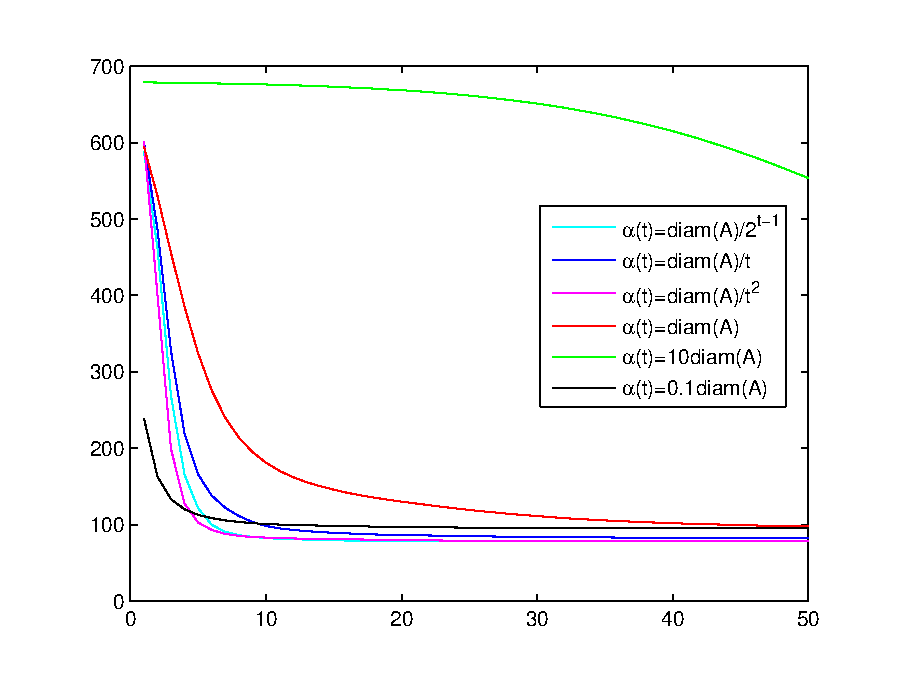
\includegraphics[width=0.6\textwidth]{dynamic_alpha_kpalm}
    \caption{Comparison of the objective values for different values of $\alpha$.}
    \label{fig:dynamic_alpha_psi_comp}
\end{figure} 

\Cref{fig:dynamic_alpha_psi_comp} shows that dynamic values of the parameter $\alpha$ which decreases fast, such as $\alpha_i(t)=
\frac{diam(\mathcal{A})}{2^{t-1}}$, achieve smaller function values.
In \Cref{fig:algs_psi_comp} we made a comparison between KPALM with dynamic rule for choosing the parameter $\alpha$, that is $\alpha_i(t)=\frac{diam(\mathcal{A})}{2^{t-1}}$, with KMEANS and KMEANS++. It demonstrates that KPALM can reach lower objective function values then KMEANS, and these are similar to the values achieved with KMEAN++. In addition, the KPALM++ are the objective function values achieved with KPALM when the $x$ variable is initialized as in KMEANS++. Unlike KMEANS, the objective function values KPALM converge to are more stable and less sensitive to its starting point.

%\begin{figure}[t]
%    \centering
%    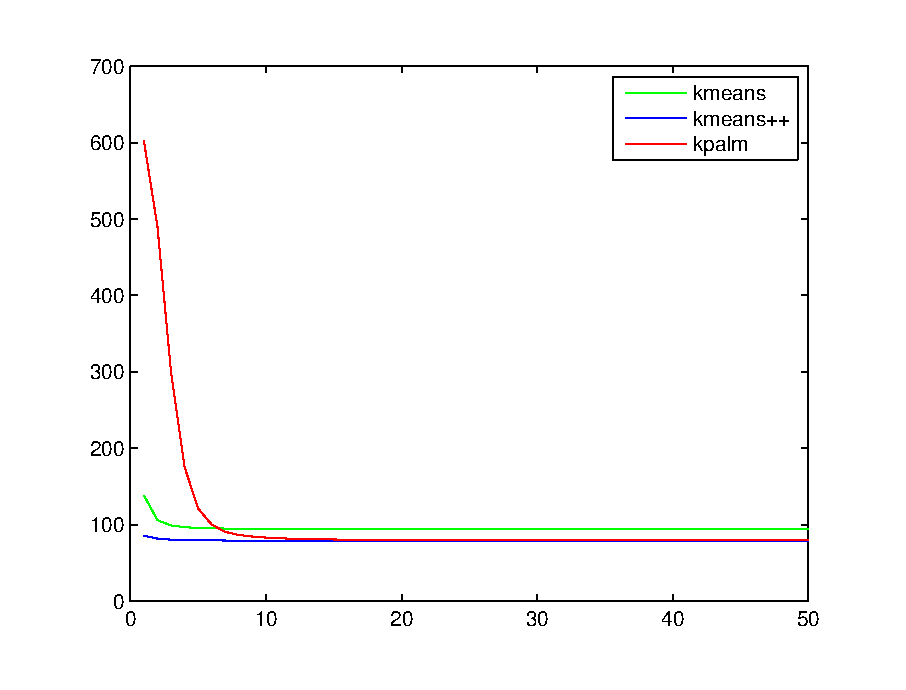
\includegraphics{psi_algs_comparison}
%    \caption{Comparison of objective function values for KMEANS, KMEANS++ and KPALM.}
%     \label{fig:algs_psi_comp}
%\end{figure}

\begin{figure}[ht]
    \centering
    \begin{subfigure}[b]{0.6\textwidth}
        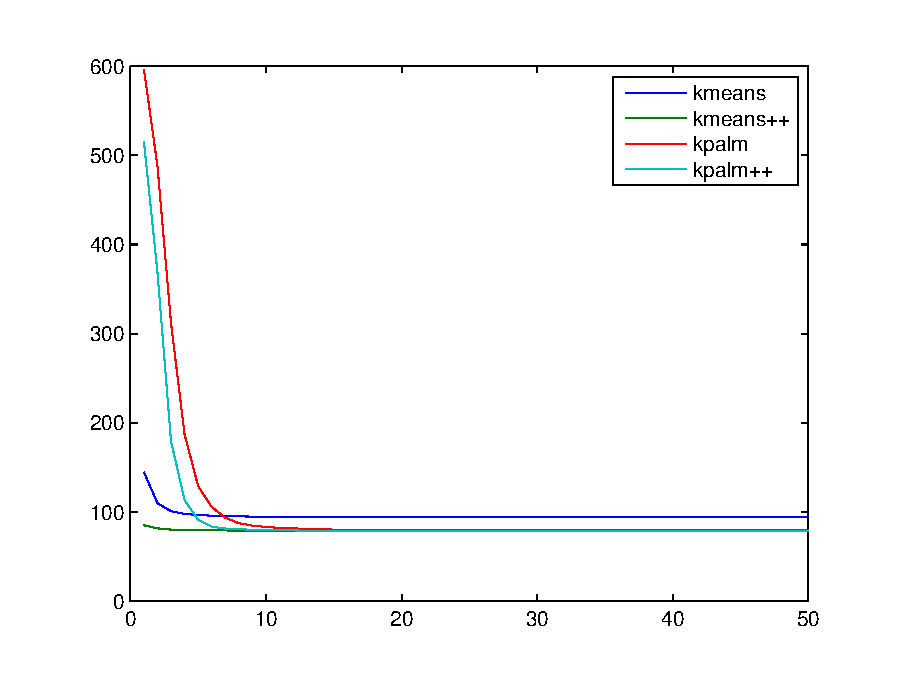
\includegraphics[width=\textwidth]{psi_algs_comparison2}
        \caption{Comparison of objective function values.}
        \label{fig:algs_psi_comp_A}
    \end{subfigure}
    \begin{subfigure}[b]{0.6\textwidth}
        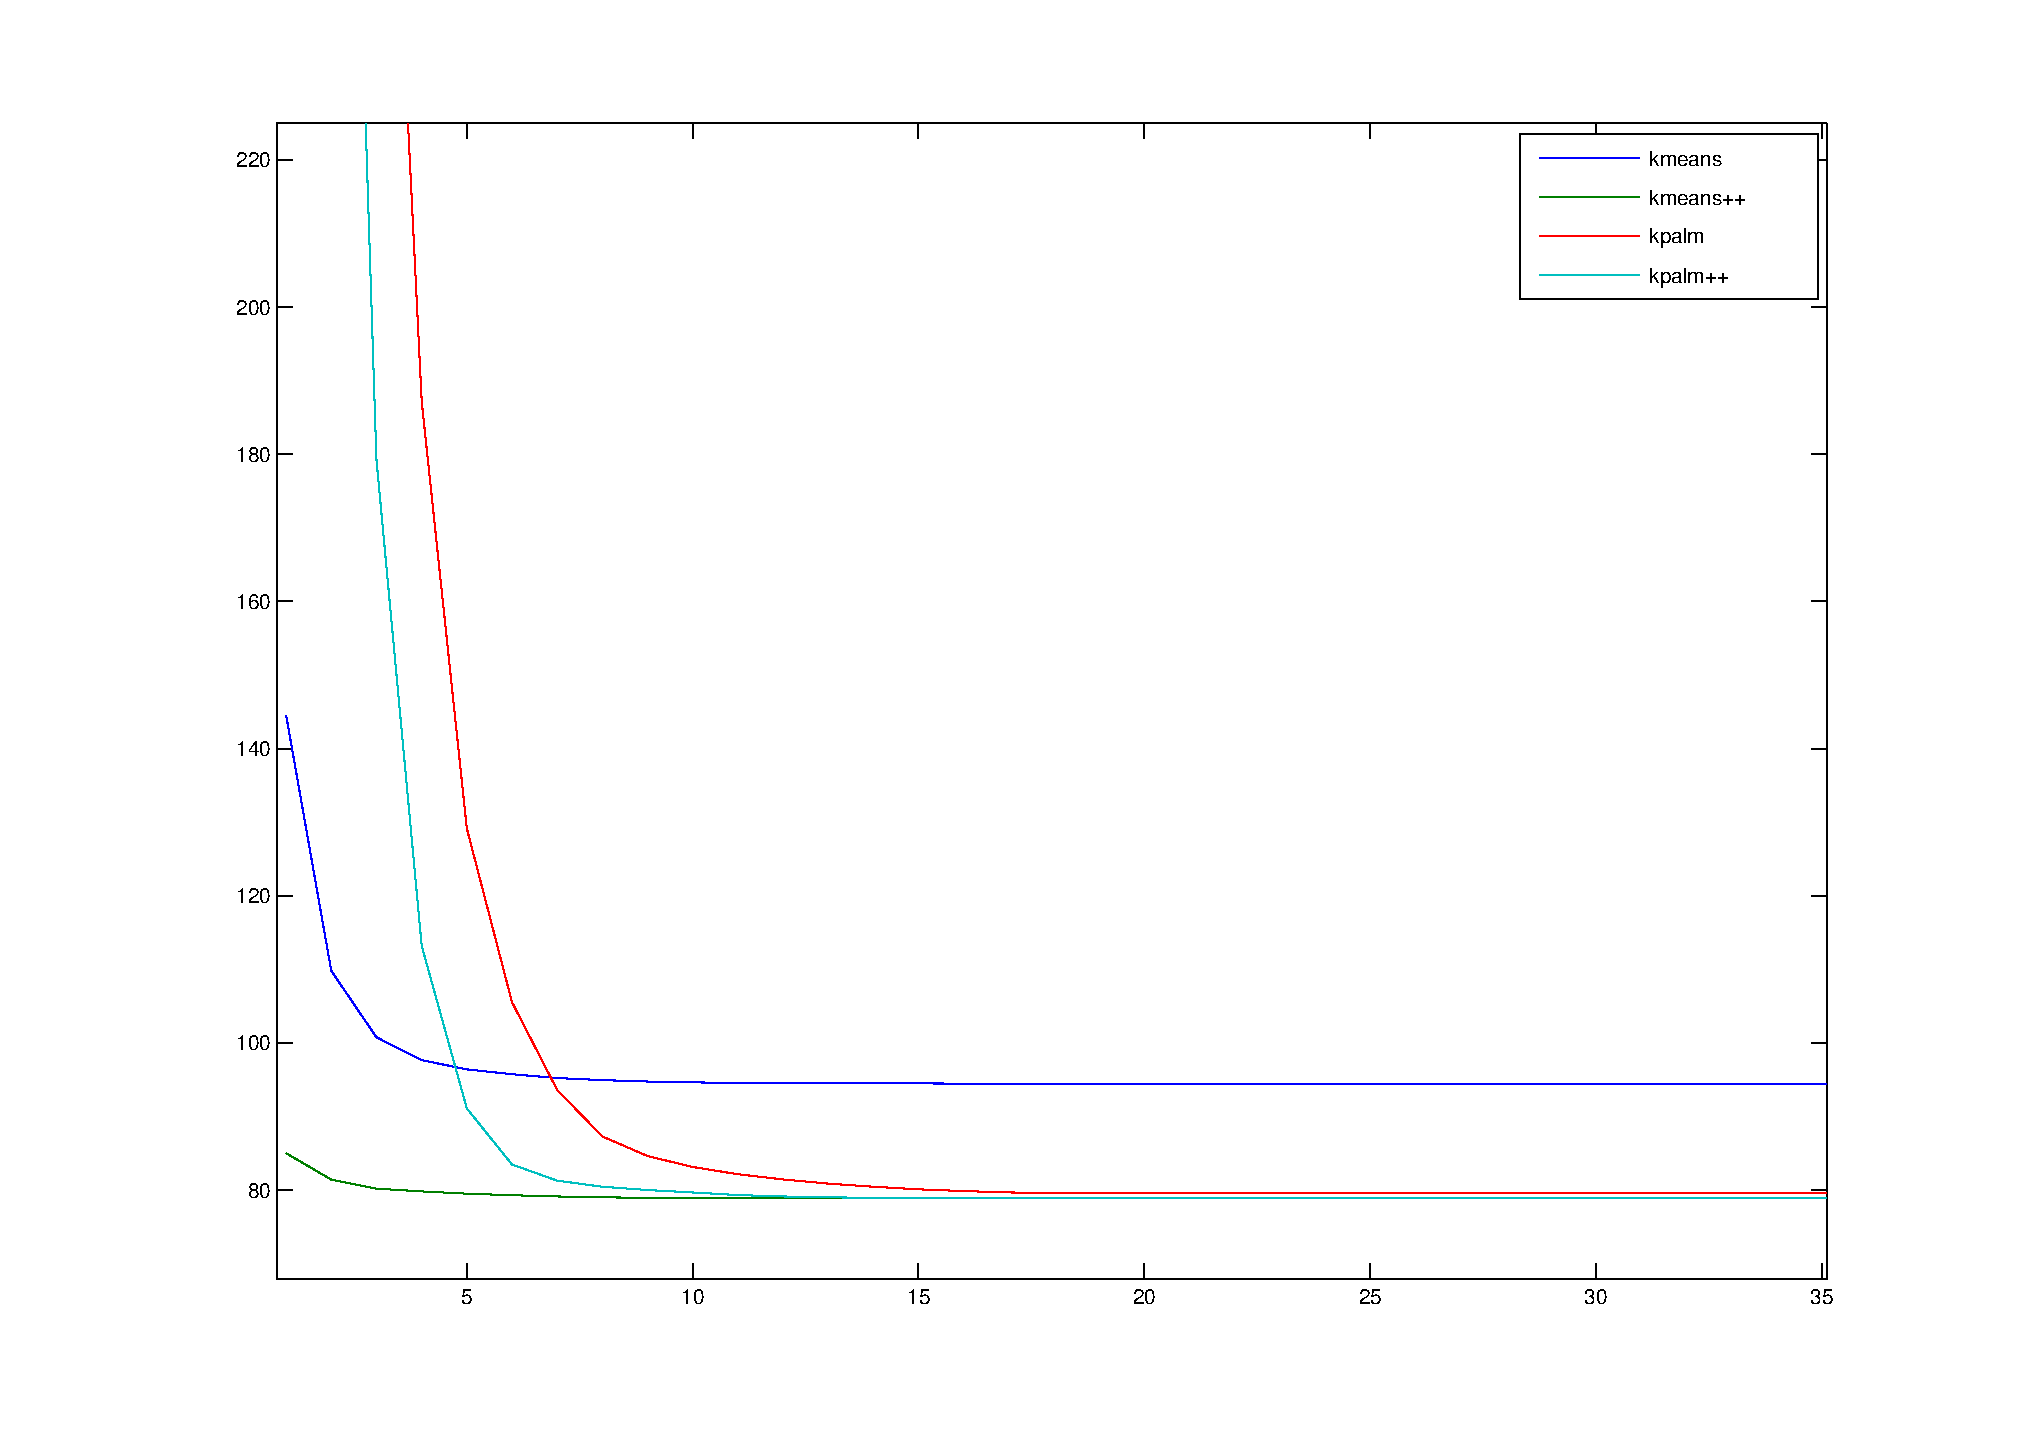
\includegraphics[width=\textwidth]{psi_algs_comparison2_zoom}
        \caption{Zoom of \Cref{fig:algs_psi_comp_A}.}
        \label{fig:algs_psi_comp_B}
    \end{subfigure}
    \caption{Comparison of objective function values for KMEANS, KMEANS++, KPALM and KMEANS++.} \label{fig:algs_psi_comp}
\end{figure}

%\begin{figure}[t]
%    \centering
%    \scalebox{.5}{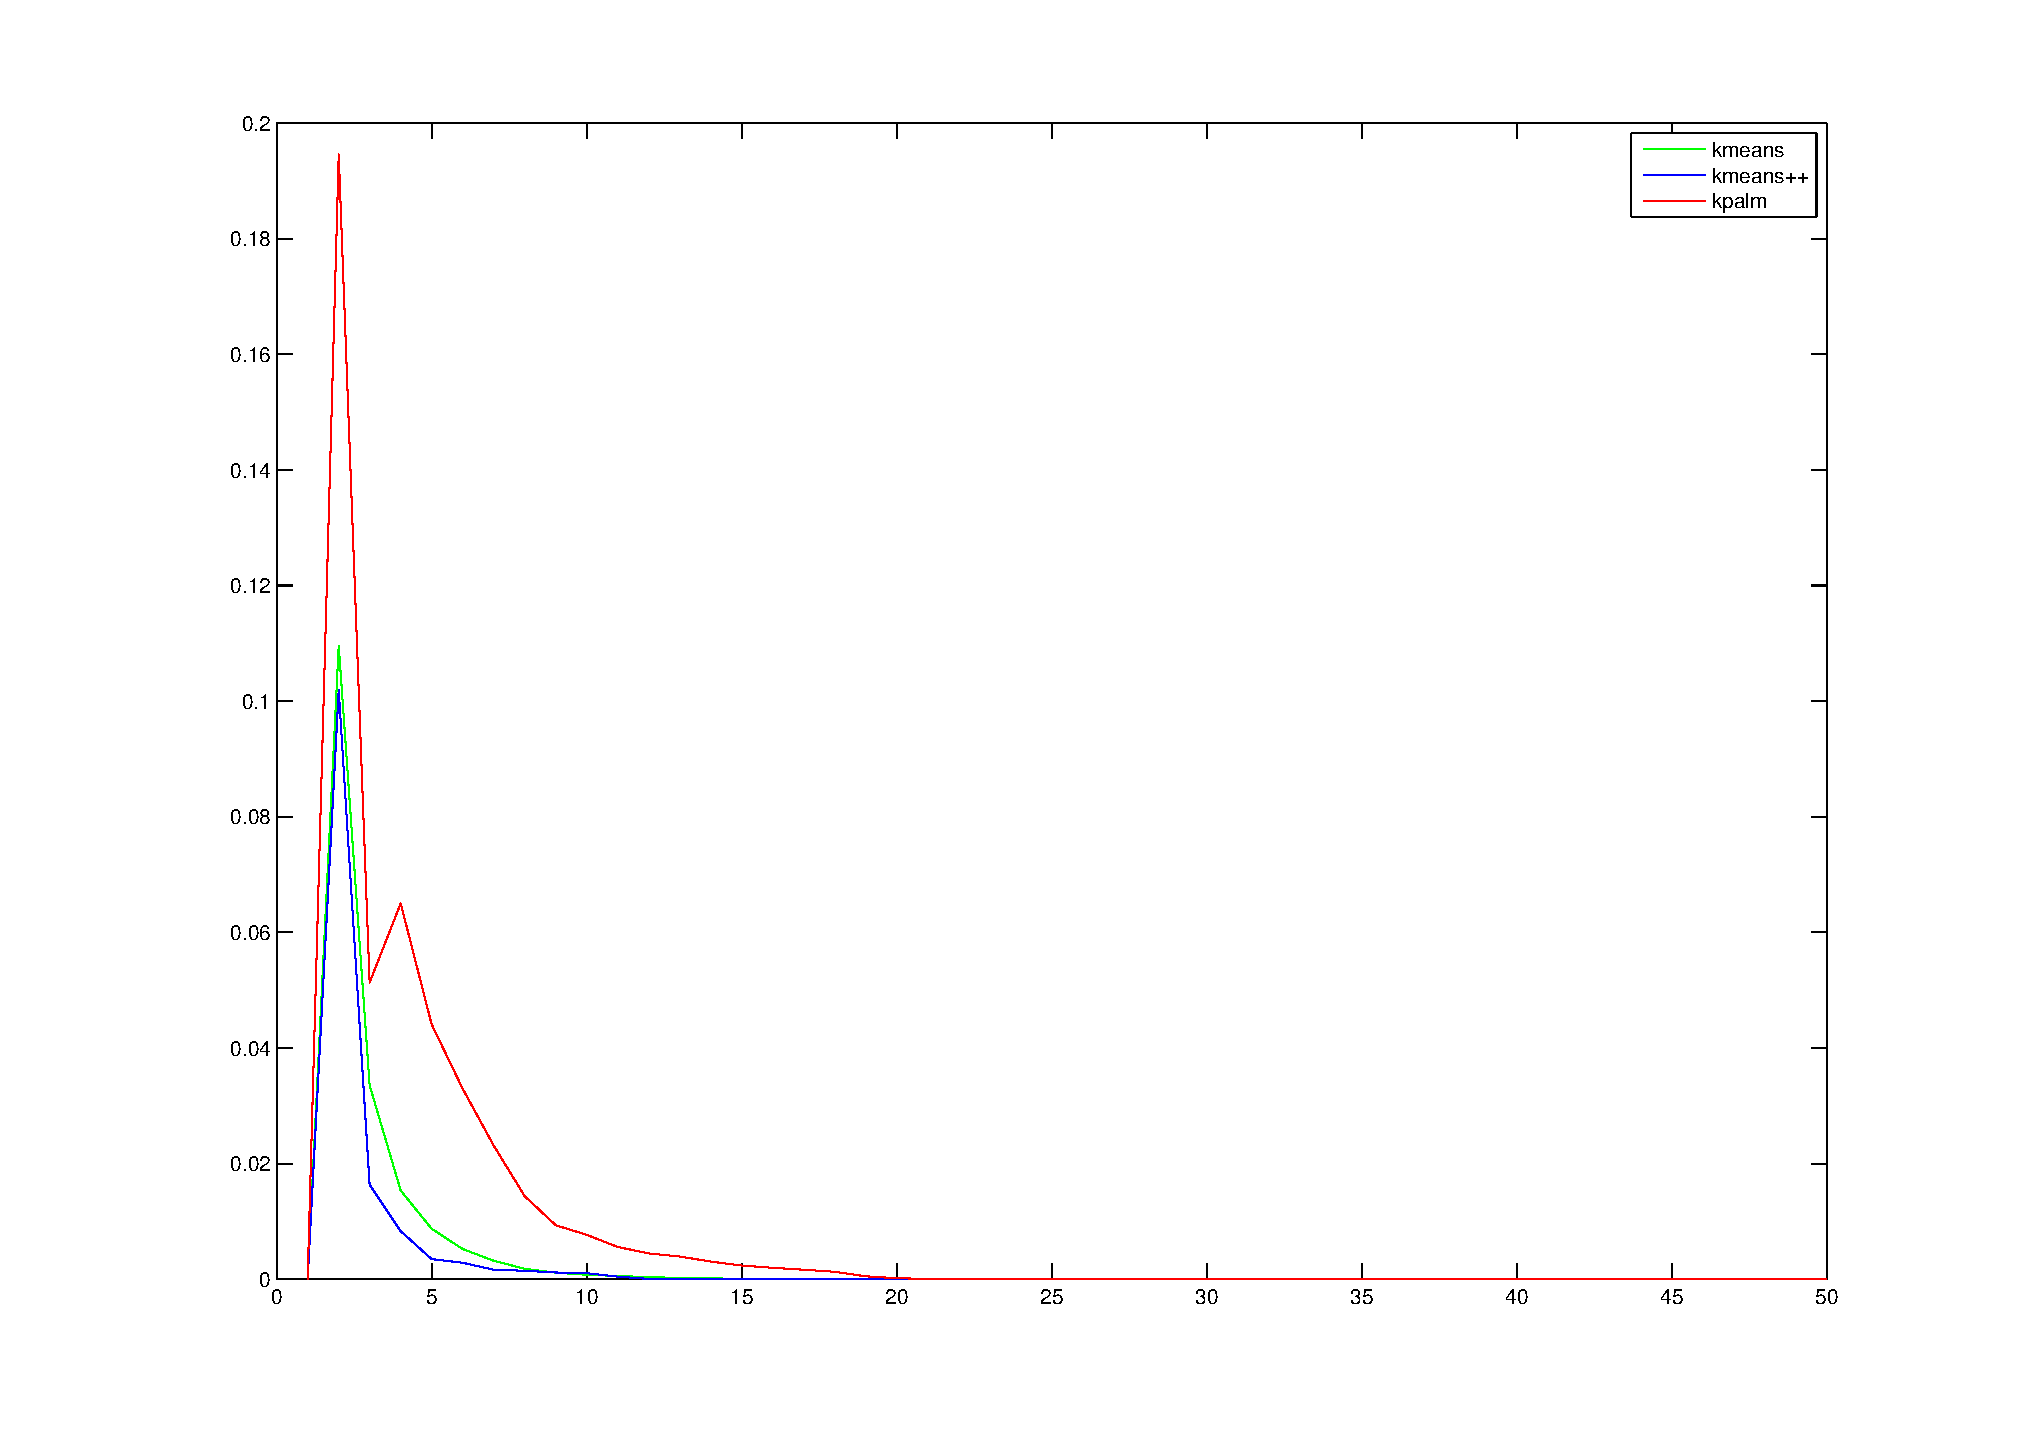
\includegraphics{relative_delta_algs_comparison}}
%    \caption{Comparison of $\frac{\|x(t+1)-x(t)\|}{\|x(t)\|}$ for KMEANS, KMEANS++ and KPALM.}
%    \label{fig:dynamic_alpha_relative_delta_comp}
%\end{figure}

\Cref{fig:iters_comp} shows the number of iteration needed to reach precision of 1e-3 between consecutive objective function values.
Similarly to \Cref{fig:dynamic_alpha_psi_comp}, in \Cref{fig:dynamic_alpha_eps_psi_comp} we can see a comparison of the objective values of $\Psi_{\varepsilon}$ for different function values. The value of $\varepsilon$ is set to be 1e-5.

\begin{figure}
    \centering
    \begin{subfigure}[b]{0.7\textwidth}
        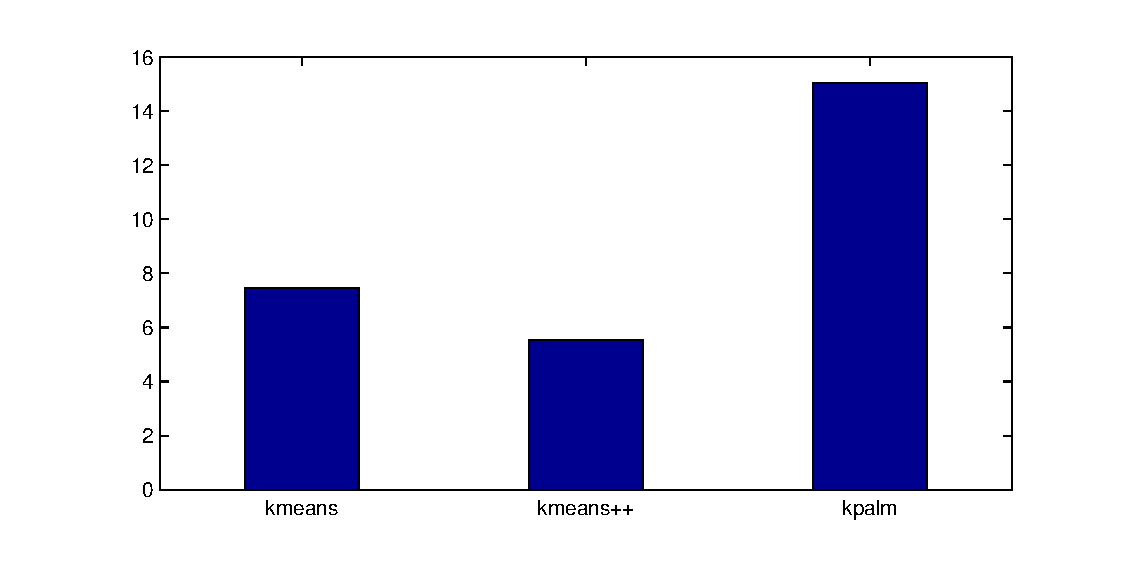
\includegraphics[width=\textwidth]{iterations_algs_comparison}
        \caption{Number of iterations of KMEANS, KMEANS++ and KPALM with $\alpha(t)=diam(\mathcal{A})/2^{t-1}$.}
        \label{fig:iters_algs_comp}
    \end{subfigure}
    ~ %add desired spacing between images, e. g. ~, \quad, \qquad, \hfill etc. 
      %(or a blank line to force the subfigure onto a new line)
    \begin{subfigure}[b]{0.7\textwidth}
        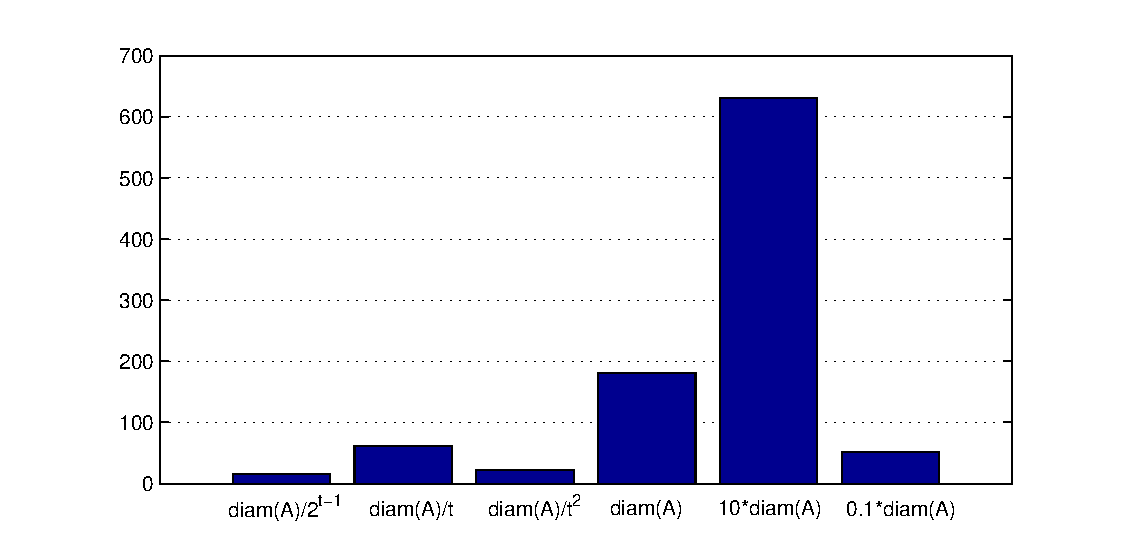
\includegraphics[width=\textwidth]{iterations_dynamic_alpha_kpalm_comparison}
        \caption{Number of iterations of KPALM with different updates of $\alpha(t)$.}
        \label{fig:iters_dyn_alpha_kpalm_comp}
    \end{subfigure}
    \begin{subfigure}[b]{0.7\textwidth}
        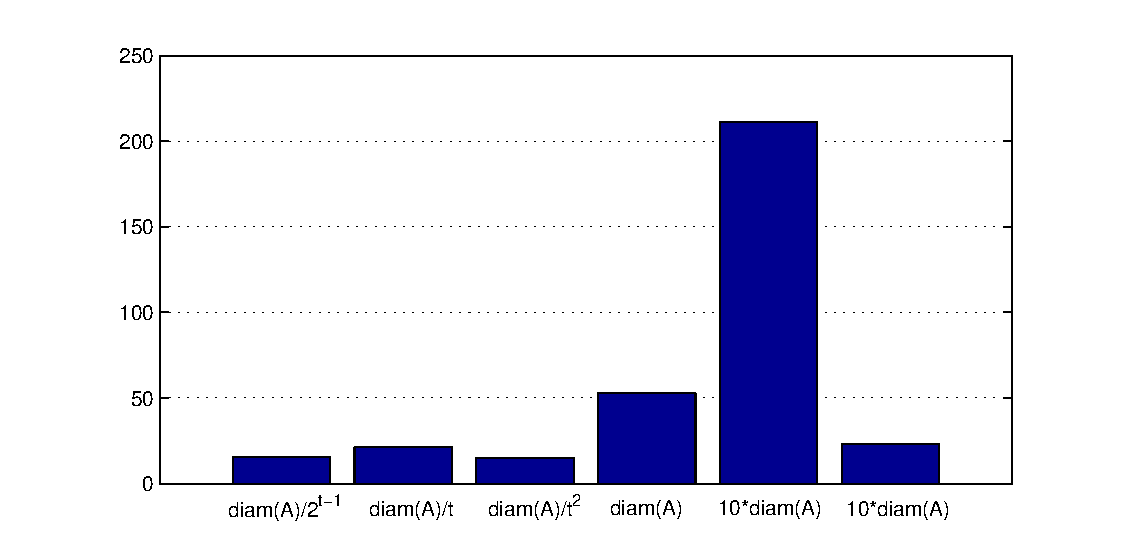
\includegraphics[width=\textwidth]{iterations_dynamic_alpha_eps_kpalm_comparison}
        \caption{Number of iterations of $\varepsilon$-KPALM with different updates of $\alpha(t)$.}
        \label{fig:iters_dyn_alpha_eps_kpalm_comp}
    \end{subfigure}
    \caption{Comparison of number of iterations needed to reach 1e-3 precision of $\Psi$.}\label{fig:iters_comp}
\end{figure}

\begin{figure}
    \centering
    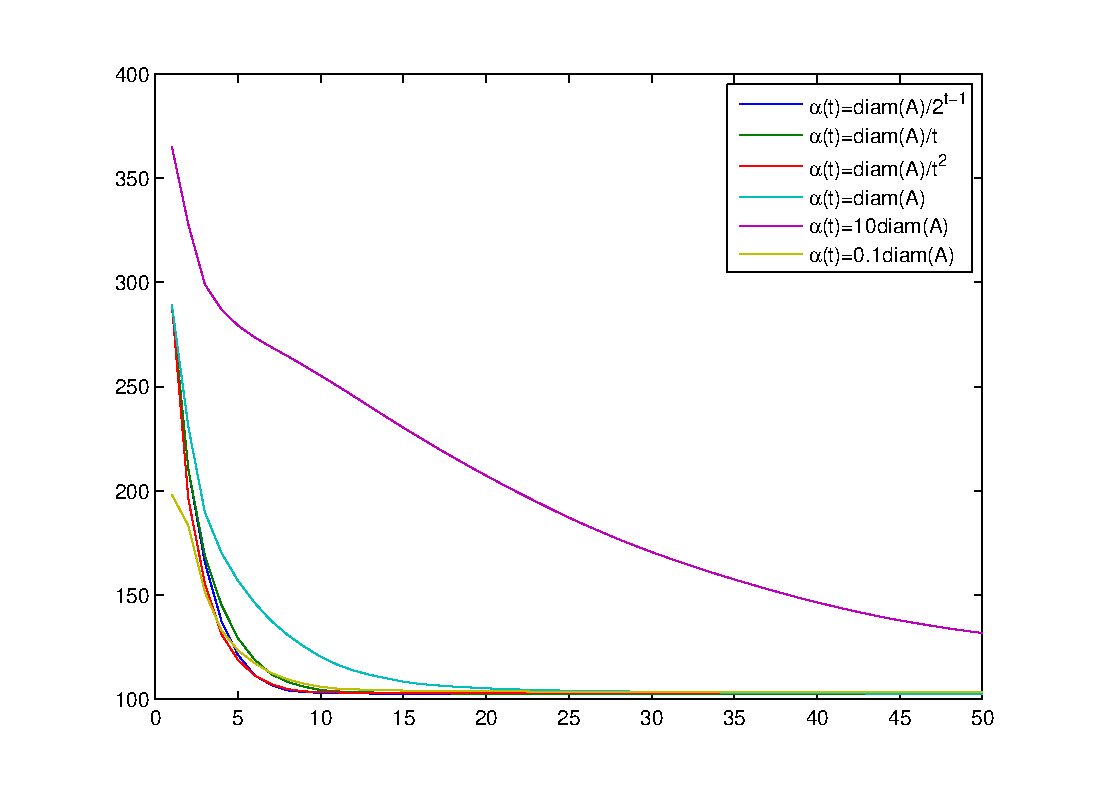
\includegraphics[width=0.75\textwidth]{dynamic_alpha_eps_kpalm}
    \caption{Comparison of the objective values for different values of $\alpha$.}
    \label{fig:dynamic_alpha_eps_psi_comp}
\end{figure}



\begin{figure}
    \centering
    \begin{subfigure}[b]{0.45\textwidth}
        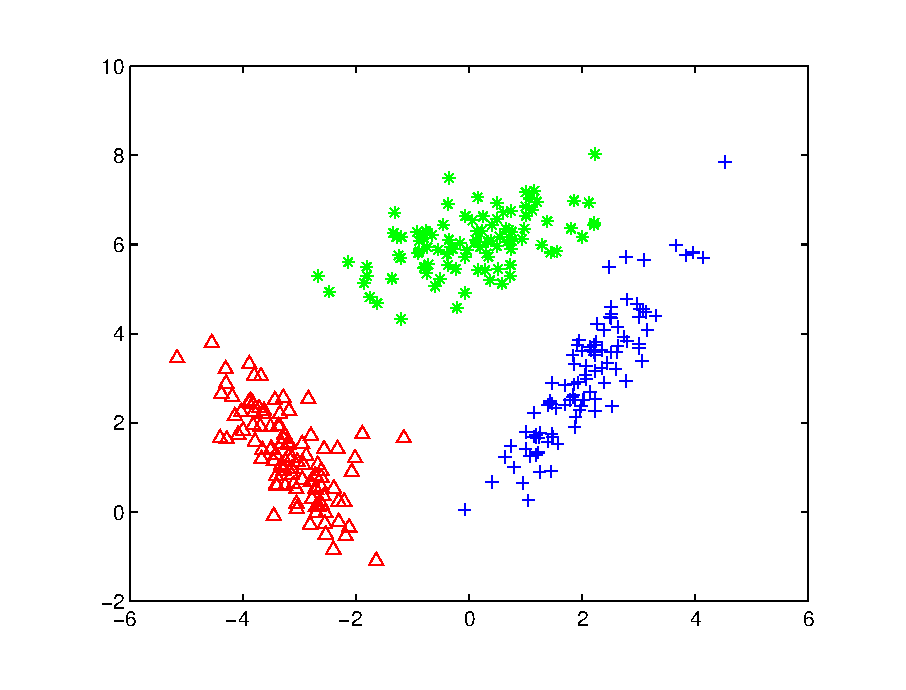
\includegraphics[width=\textwidth]{dense_gaussians}
        \caption{Dense Gaussians.}
        \label{fig:dense_gaussians}
    \end{subfigure}
    \quad
    \begin{subfigure}[b]{0.45\textwidth}
        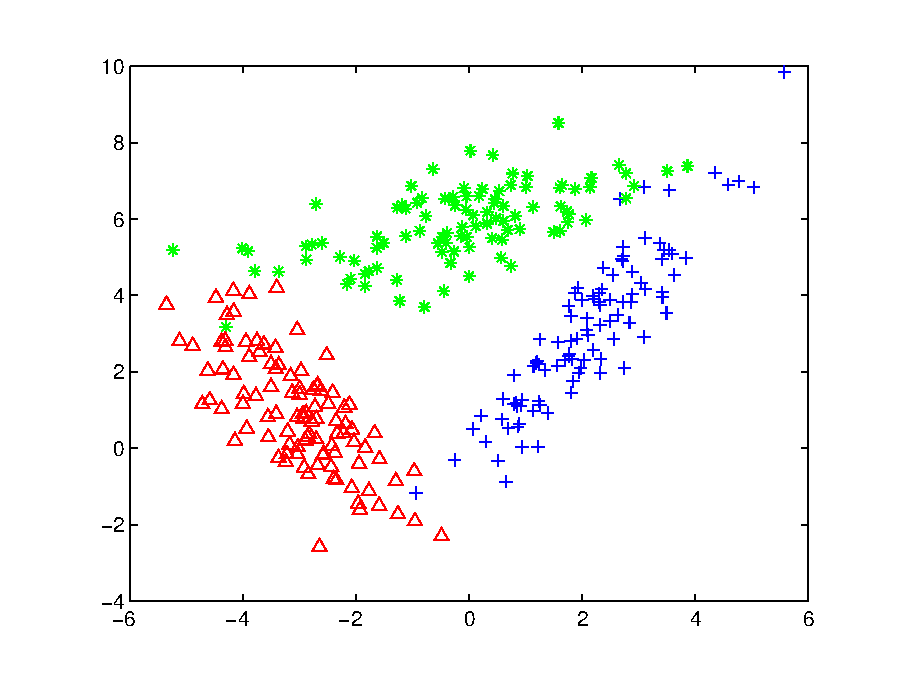
\includegraphics[width=\textwidth]{sparse_gaussians}
        \caption{Sparse Gaussians.}
        \label{fig:sparse_gaussians}
    \end{subfigure}
    \caption{Two datasets, each 300 points.}
    \label{fig:gaussians}
\end{figure}

\begin{figure}
    \centering
    \begin{subfigure}[b]{0.45\textwidth}
        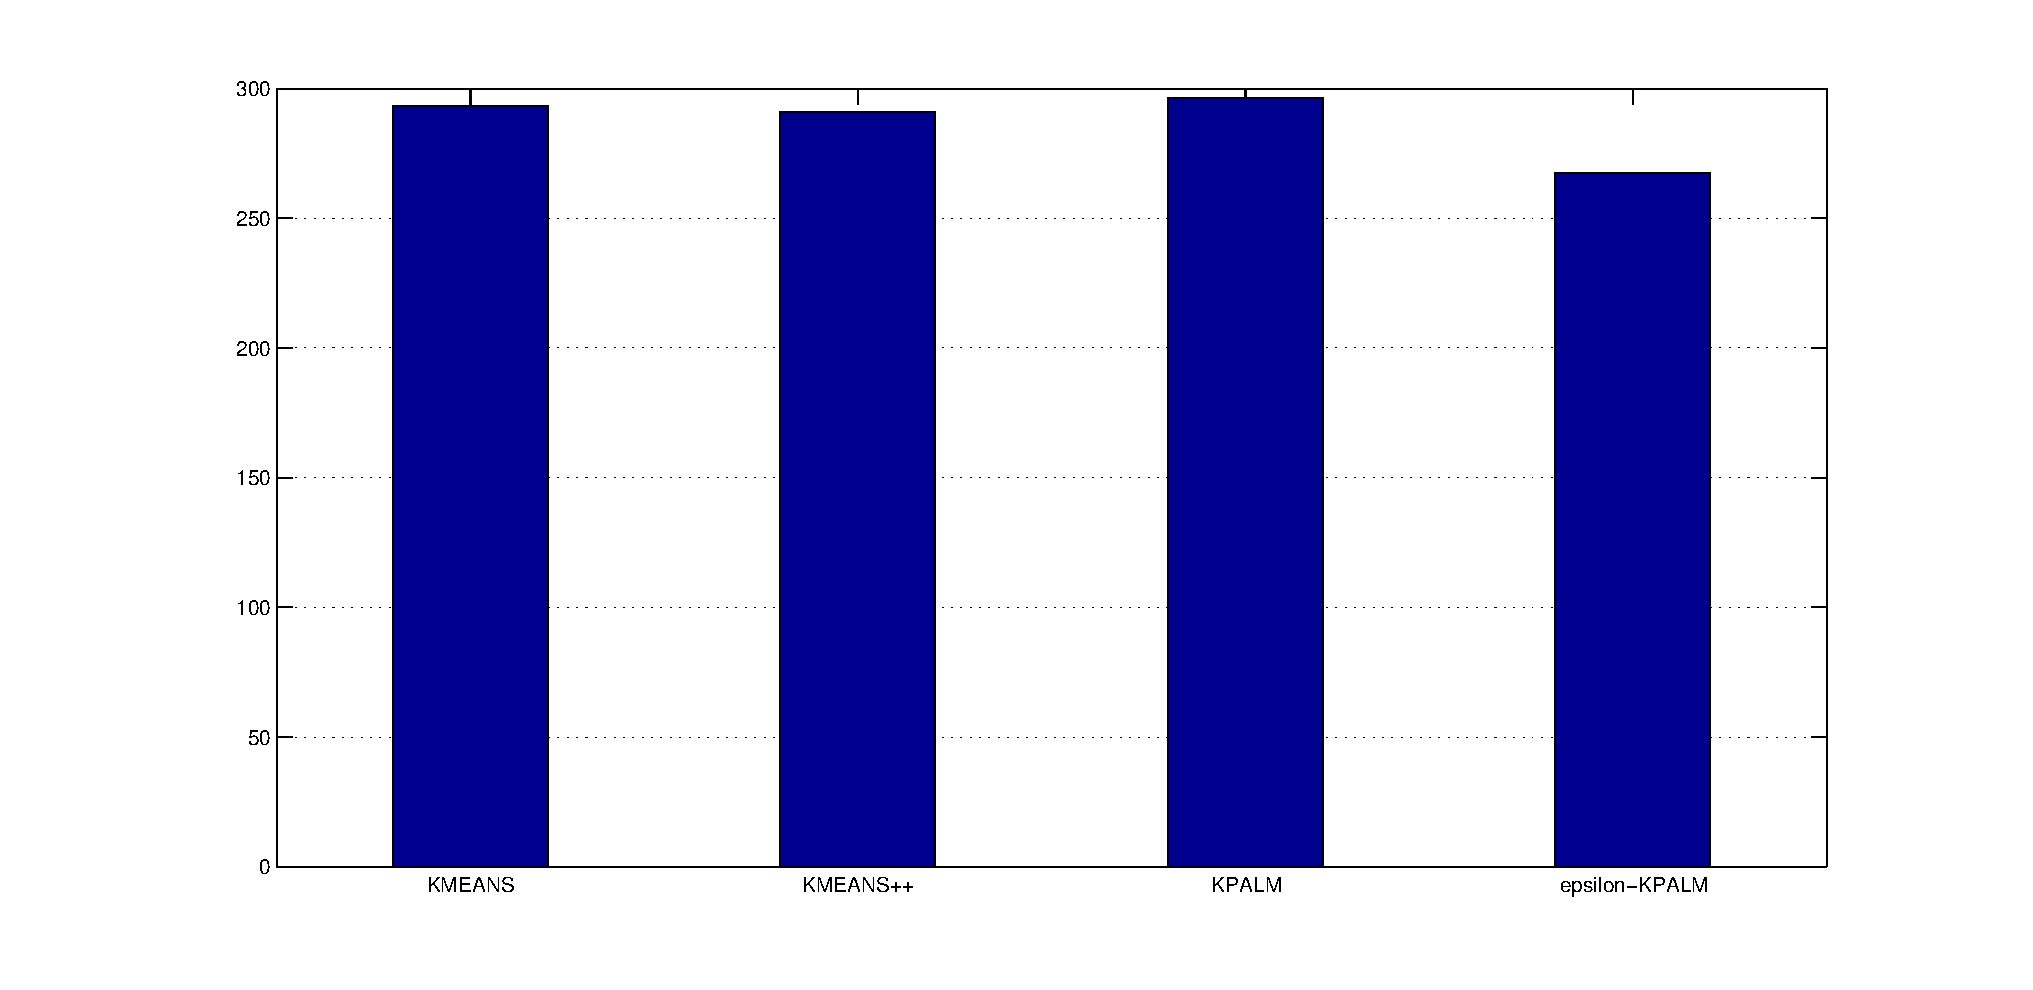
\includegraphics[width=\textwidth]{dense_gaussians_similarity}
        \caption{Dense Gaussians clustering.}
        \label{fig:dense_gaussians_similarity}
    \end{subfigure}
    \quad
    \begin{subfigure}[b]{0.45\textwidth}
        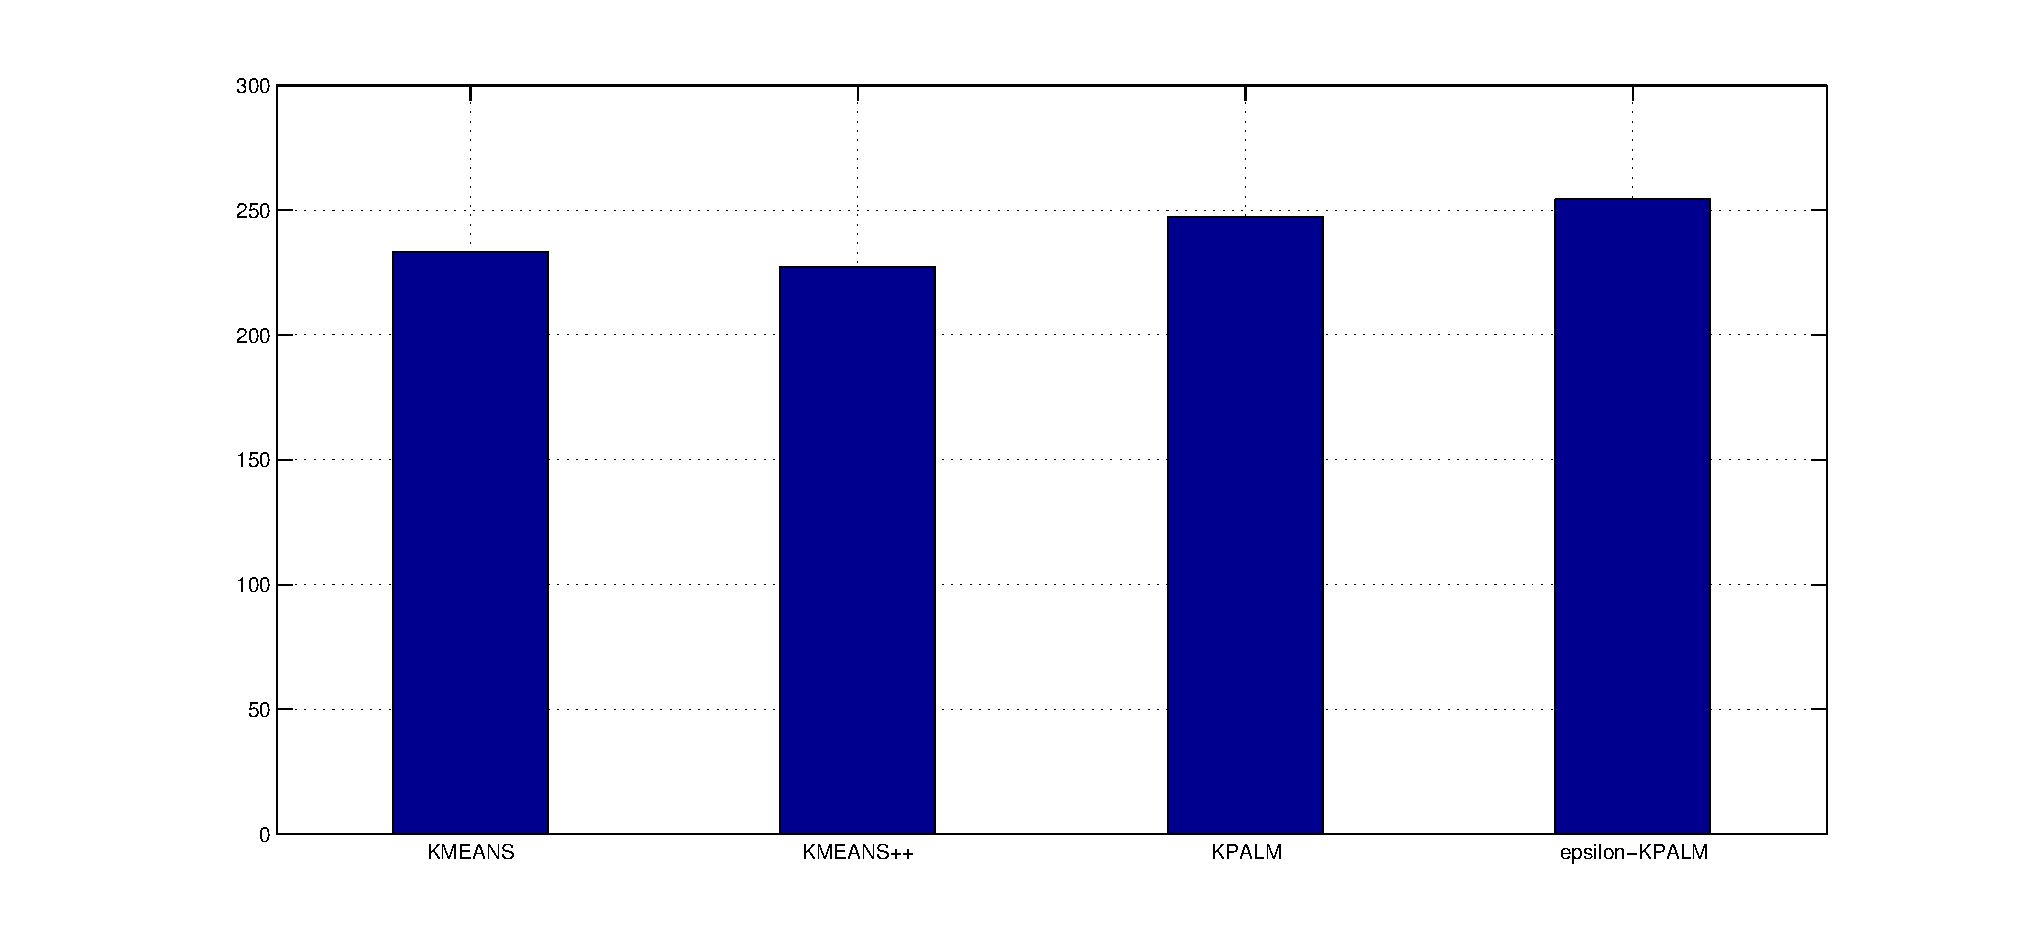
\includegraphics[width=\textwidth]{sparse_gaussians_similarity}
        \caption{Sparse Gaussians clustering.}
        \label{fig:sparse_gaussians_similarity}
    \end{subfigure}
    \caption{Results of clustering algorithms for dense and sparse datasets.}
    \label{fig:gaussians_similarity}
\end{figure}

\begin{figure}
    \centering
    \begin{subfigure}[b]{0.95\textwidth}
        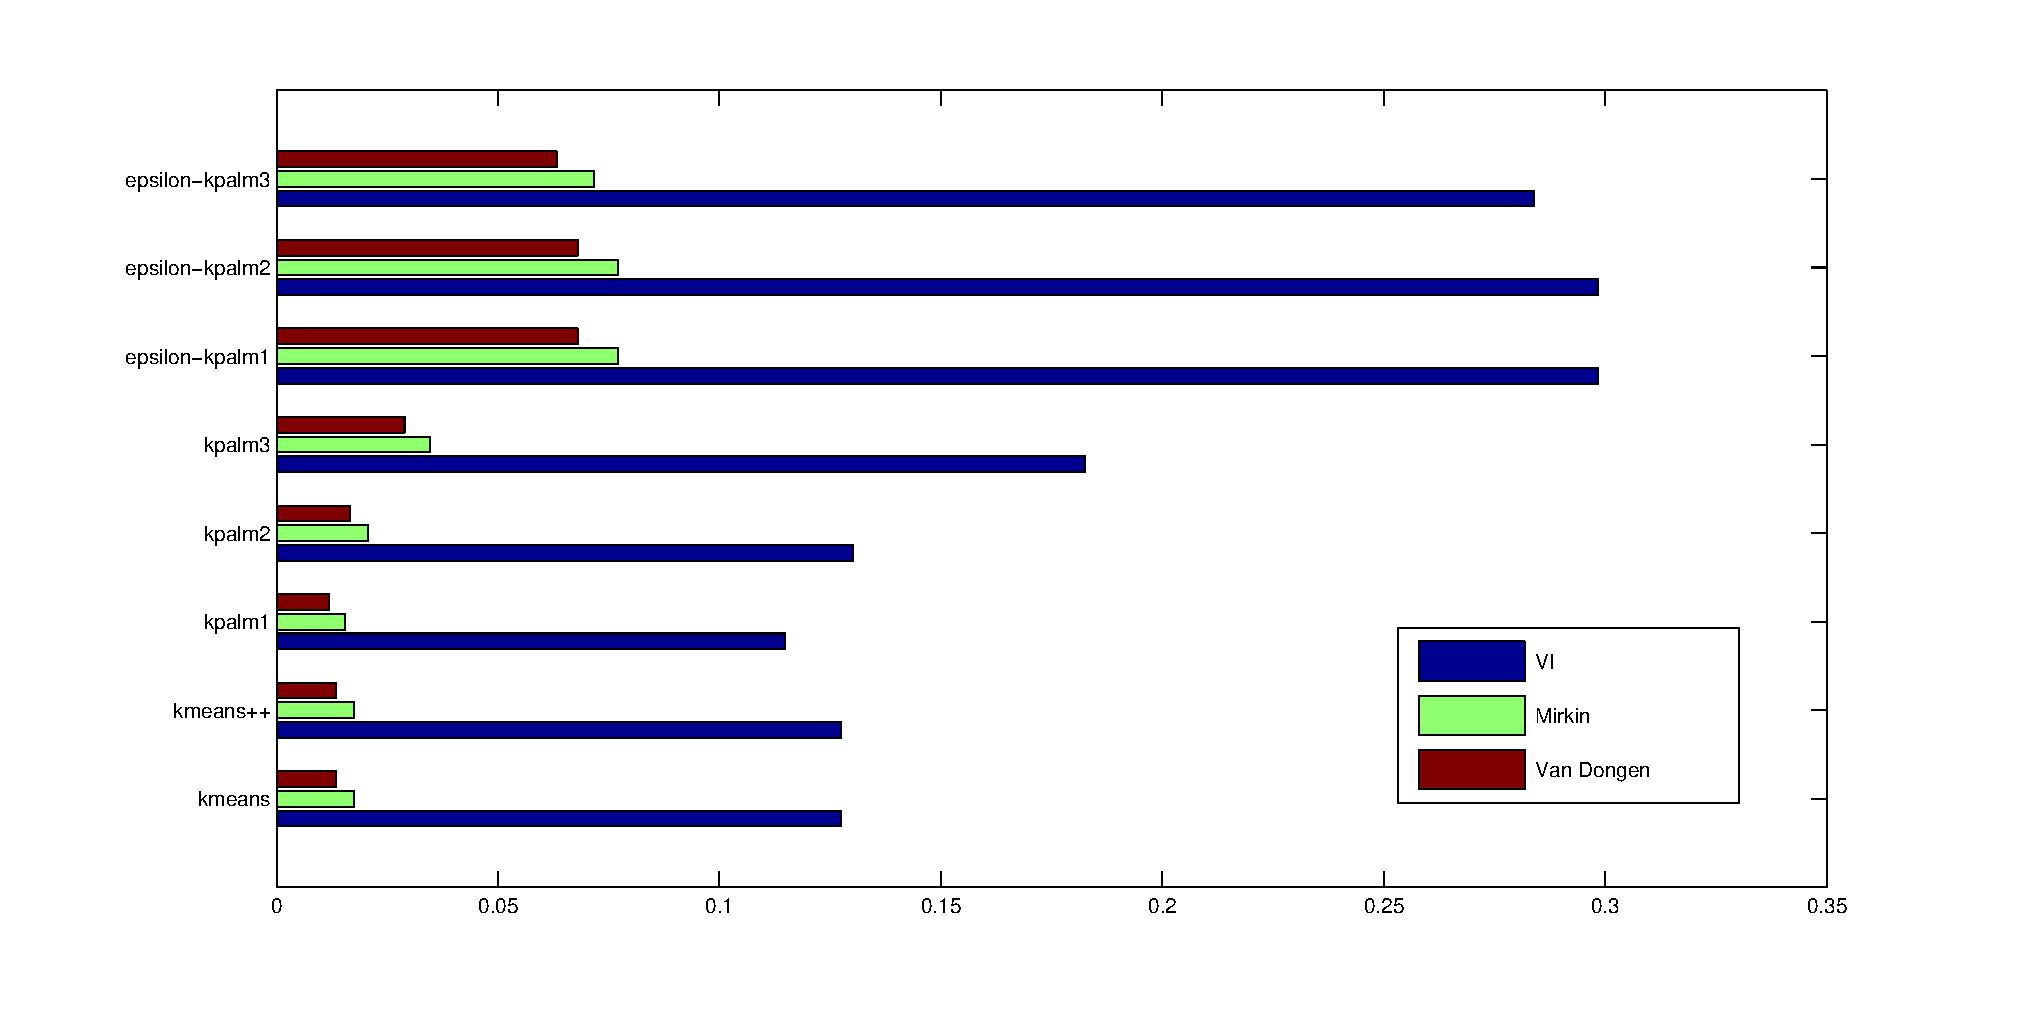
\includegraphics[width=\textwidth]{dense_gaussians_metrics2}
        \caption{Dense Gaussians metrics comparison.}
        \label{fig:dense_gaussians_metrics}
    \end{subfigure}
    \quad
    \begin{subfigure}[b]{0.95\textwidth}
        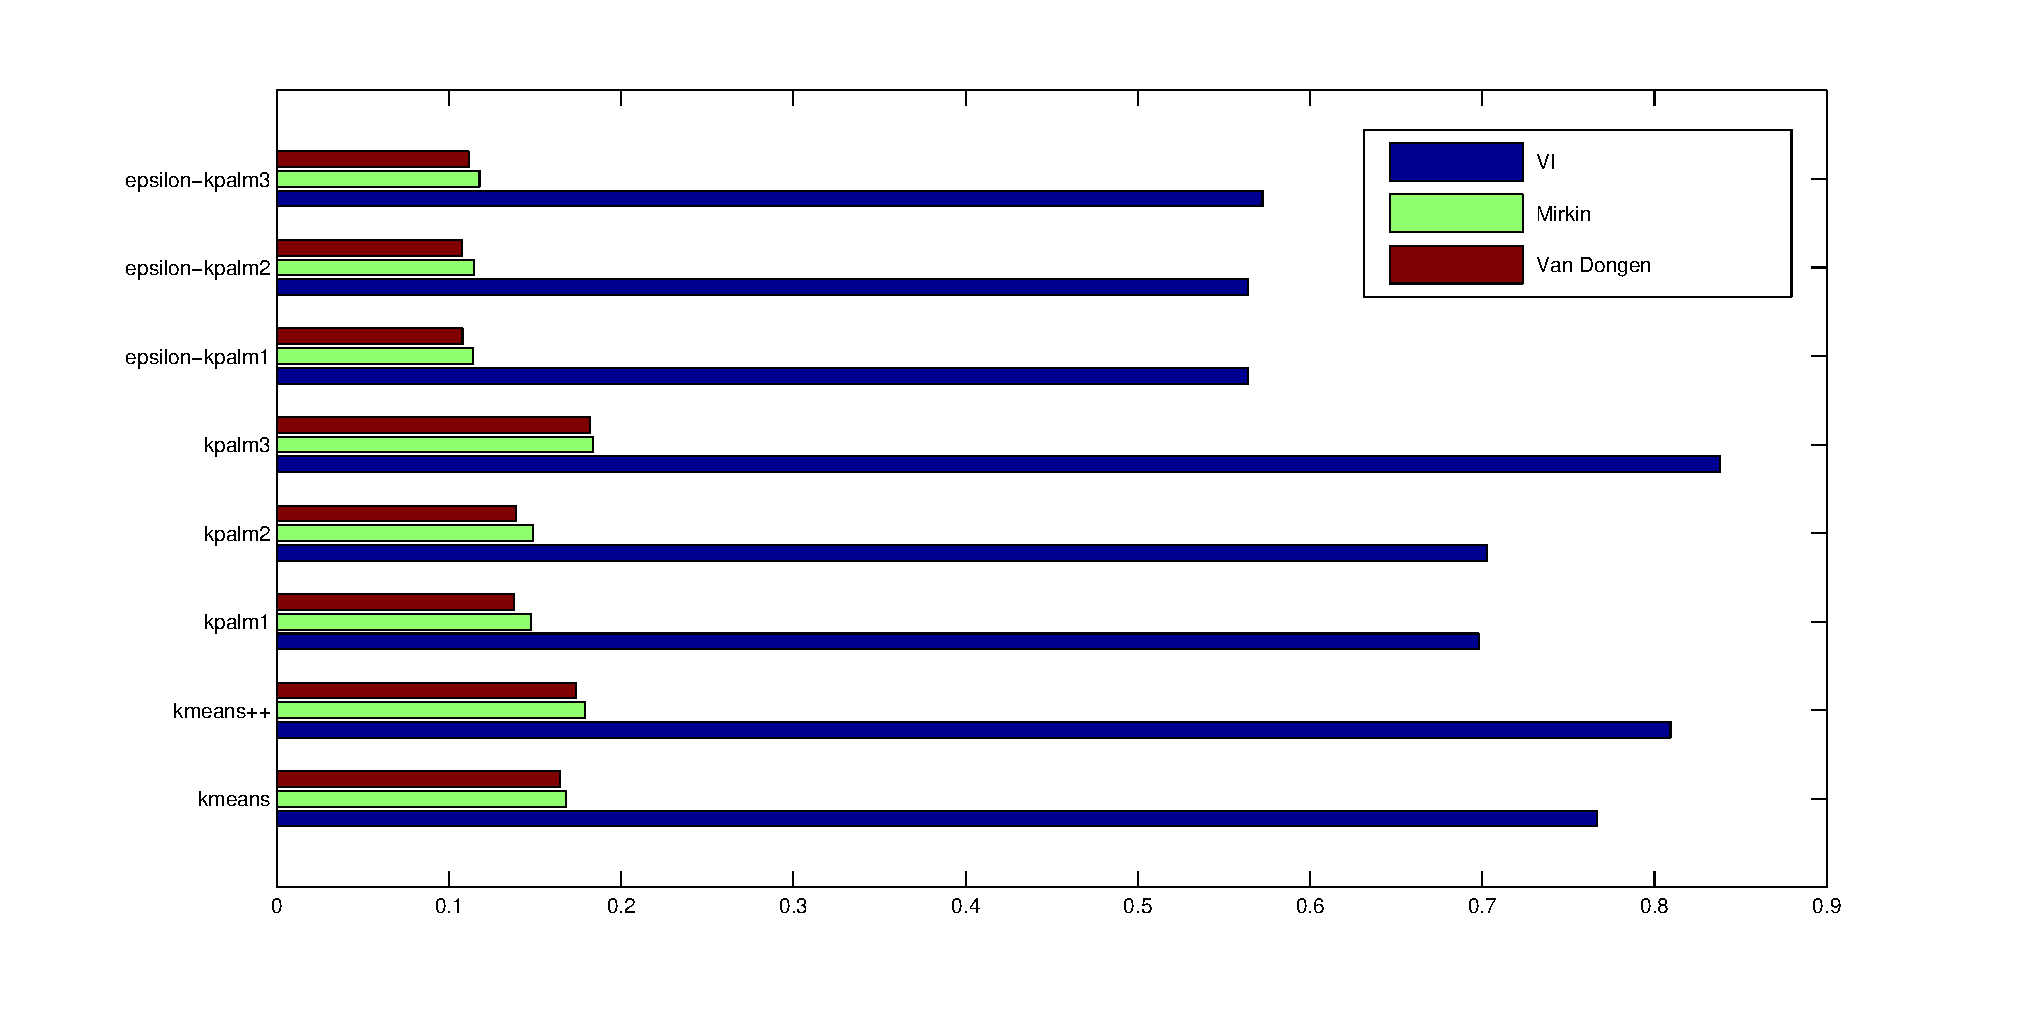
\includegraphics[width=\textwidth]{sparse_gaussians_metrics2}
        \caption{Sparse Gaussians metrics comparison.}
        \label{fig:sparse_gaussians_metrics}
    \end{subfigure}
    \caption{Comparison of metrics between clusterings for dense and sparse datasets.}
    \label{fig:gaussians_metrics}
\end{figure}

\subsection{Synthetic Dataset}

In this section we show that $\varepsilon$-KPALM is less sensitive to outliners in the data verses algorithms that suit the squared Euclidean norm (e.g., KMEANS, KMEANS++ and KPALM). We generated two synthetic datasets, each contains 300 points in the plane, by sampling three two-dimensional Gaussian, 100 samples each. In \Cref{fig:gaussians}(\ref{fig:dense_gaussians}) the clusters are denser than in \Cref{fig:gaussians}(\ref{fig:sparse_gaussians}).
Then we run the clustering algorithms and compared their clustering results, namely, how many points were clustered correctly. From \Cref{fig:gaussians_similarity}(\ref{fig:dense_gaussians_similarity}) it is evident that KMEANS is superior to other algorithms in the dense case and $\varepsilon$-KPALM is quite sensitive. Whereas, in the sparse case in \Cref{fig:gaussians_similarity}(\ref{fig:sparse_gaussians_similarity}), $\varepsilon$-KPALM is superior, and less sensitive to outliners. In \Cref{fig:gaussians_metrics} we compare the distance of clusterings achieved with different algorithms to the desired clustering, where kpalm1, kpalm2 and kpalm3 match using $\alpha(t)=diam(\mathcal{A})/2^{t-1}$, $\alpha(t)=diam(\mathcal{A})/t^2$ and $\alpha(t)=diam(\mathcal{A})$ respectively, and similarly for $\varepsilon$-kpalm$i$, $i \in \{1,2,3\}$. In \Cref{fig:gaussians_metrics}(\ref{fig:dense_gaussians_metrics}) we witness that for dense dataset, the resulting clusterings of squared Euclidean algorithms, namely, KMEANS, KMEANS++ and KPALM, are superior to the clustering $\varepsilon$-KPALM, where KPALM with $\alpha(t)=diam(\mathcal{A})/2^{t-1}$ gives the best result, that is, the clustering in this setting is the closest to the desired clustering. Whereas in the sparse dataset, the clustering achieved with $\varepsilon$-KPALM with $\alpha(t)=diam(\mathcal{A})/t^2$ is the closest to the desired clustering, as reflected from \Cref{fig:gaussians_metrics}(\ref{fig:sparse_gaussians_metrics}).

%\section{Clustering via ADMM Approach}
%
%Introducing some new variable into the problem leads to the following clustering problem notation
%\begin{equation*}
%\begin{split}
%	&\min\limits_{x \in \mathbb{R}^{nk}} \min\limits_{w \in \mathbb{R}^{km}} \left\lbrace \sum\limits_{i=1}^{m} \sum\limits_{l=1}^{k} w^i_l d(x^l,a^i) \mid w^i \in \Delta, i=1,2, \ldots, m \right\rbrace \\
%	&= \min\limits_{x \in \mathbb{R}^{nk}, w \in \mathbb{R}^{km}, z \in \mathbb{R}^{km}} \left\lbrace \sum\limits_{i=1}^{m} \sum\limits_{l=1}^{k} w^i_l z^i_l \: \bigg| 
%\begin{array}{c c c}
% w^i \in \Delta, & i=1,2, \ldots, m, & \\
% z^i_l = d(x^l,a^i), & i=1,2, \ldots, m, & l=1,2, \ldots, k
%\end{array}
%\right\rbrace .
%\end{split}
%\end{equation*}
%
%The augmented Lagrangian that is associated with this problem is 
%\begin{equation}
%	L_{\rho}(w,x,z,y) = \sum\limits_{i=1}^{m} \sum\limits_{l=1}^{k} w^i_l z^i_l + \sum\limits_{i=1}^{m} \sum\limits_{l=1}^{k} y^i_l (z^i_l - d(x^l,a^i)) + \frac{\rho}{2} \sum\limits_{i=1}^{m} \sum\limits_{l=1}^{k} \left(z^i_l - d(x^l,a^i)\right)^2 . \label{StateEq59}
%\end{equation}
%Thus the ADMM formulas for (\ref{StateEq60}) are as follows
%\begin{equation*}
%\begin{split}
%	w(t+1) &= \arg\!\min\limits_{w \in \Delta^m} L_{\rho}(w,x(t),z(t),y(t)), \\
%	\Rightarrow \quad w^i(t+1) &= \arg\!\min\limits_{w^i \in \Delta} \sum\limits_{l=1}^{k} w^i_l z^i_l(t) = \arg\!\min\limits_{w^i \in \Delta} \left\langle w^i, z^i(t) \right\rangle, \quad 1 \leq i \leq m , \\
%	x(t+1) &= \arg\!\min\limits_{x \in \mathbb{R}^{nk}} L_{\rho}(w(t+1),x,z(t),y(t)), \\
%	\Rightarrow \quad x^l(t+1) &= \arg\!\min\limits_{x^l \in \mathbb{R}^{nk}} -\sum\limits_{i=1}^{m} y^i_l(t) d(x^l, a^i) + \frac{\rho}{2} \sum\limits_{i=1}^{m} \left(z^i_l - d(x^l,a^i)\right)^2, \quad 1 \leq l \leq k , \\
%	z(t+1) &= \arg\!\min\limits_{z \in \mathbb{R}^{km}} L_{\rho}(w(t+1),x(t+1),z,y(t)), \\
%	\Rightarrow \quad z^i(t+1) &= \arg\!\min\limits_{z^i \in \mathbb{R}^{km}} \left\langle w^i(t+1), z^i \right\rangle +  \left\langle y^i(t), z^i \right\rangle + \frac{\rho}{2} \left\lVert z^i - \left( d(x^l(t+1), a^i \right)_{l=1, \ldots , k} \right\lVert^2 \\
%	&= \left(d(x^l(t+1), a^i \right)_{l=1, \ldots , k} - \frac{1}{\rho}\left( w^i(t+1) + y^i(t) \right), \quad 1 \leq i \leq m, \\
%	y^i_l(t+1) &= y^i_l(t) + \rho (z^i_l(t+1) - d(x^l(t+1), a^i), \quad 1 \leq i \leq m, \: 1 \leq l \leq k.
%\end{split}
%\end{equation*}

\clearpage

\begin{thebibliography}{99}
\bibitem{AB2009} Attouch, H., Bolte, J.: On the convergence of the proximal algorithm for nonsmooth functions involving analytic features. Math. Program. \textbf{116}, 5-16 (2009)
%
\bibitem{ABS2013} Attouch, H., Bolte, J., Svaiter, B.F.: Convergence of descent methods for semi-algebraic and tame problems: proximal algorithms, forward–backward splitting, and regularized Gauss–Seidel methods. Math. Program. \textbf{137}, 91-129 (2013)
%
\bibitem{BS2015} Beck, A., Sabach, S.: Weiszfeld’s Method: Old and New Results. Journal of Optimization Theory and Applications \textbf{164}, 1-40 (2015)
%
\bibitem{ATY1991} Ben-Tal, A., Teboulle, M., Yang, W.H.: A least-squares-based method for a class of nonsmooth minimization problems with applications in plasticity. Applied Mathematics and Optimization \textbf{24}, 273-288 (1991)
%
\bibitem{BST2014} Bolte, J., Sabach, S., Teboulle, M.: Proximal alternating linearized minimization for nonconvex and nonsmooth problems. Math. Program. \textbf{146}, 459-494 (2014)
%
\bibitem{M2005} Meila, M.: Comparing Clusterings – An Axiomatic View. In ICML '05: Proceedings of the 22nd international conference on Machine Learning ACM, New York, 577-584 (2005)
%
\bibitem{SI1984} Selim, S.Z., Ismail, M. A.: K-Means-Type Algorithms: A Generalized Convergence Theorem and Characterization of Local Optimality. IEEE Transactions on Pattern Analysis and Machine Intelligence \textbf{6}, 81-87 (1984)
%
\bibitem{T2007} Teboulle, M.: A Unified Continuous Optimization Framework for Center-Based Clustering Methods. The Journal of Machine Learning Research \textbf{8}, 65-102 (2007)
\end{thebibliography}

\end{document}
